% MDPI JMSE submission-format draft converted from the PaperForge Geo manuscript.
\documentclass[jmse,article,submit,moreauthors]{Definitions/mdpi}

% Dates and publisher metadata are intentionally left commented for submission-stage drafting.
\firstpage{1}
\makeatletter
\setcounter{page}{\@firstpage}
\makeatother
\pubvolume{1}
\issuenum{1}
\articlenumber{0}
\pubyear{2026}
\copyrightyear{2026}
%\datereceived{}
%\daterevised{}
%\dateaccepted{}
%\datepublished{}
%\doinum{}

\usepackage{booktabs}
\usepackage{multirow}
\usepackage{float}
\usetikzlibrary{arrows.meta,calc}
\graphicspath{{pic/}}
\setlength{\headheight}{20pt}
\emergencystretch=2em
% Keep figure-only pages journal-like: MDPI/LaTeX otherwise vertically centers
% lone floats, which creates large blank bands above compact heatmaps.
\makeatletter
\setlength{\@fptop}{0pt}
\setlength{\@fpsep}{8pt plus 1fil}
\setlength{\@fpbot}{0pt plus 1fil}
\makeatother
% Hide submission-date and copyright fields in this draft copy.  The MDPI
% class builds these items in a first-page left column; disabling that block is
% cleaner for a pre-submission PDF than leaving empty Received/Published labels.
\makeatletter
\providecommand{\@datepublished}{}
\renewcommand{\leftcolDates}{}
\renewcommand{\leftcolumnCright}{}
\renewcommand{\contentleftcolumn}{}
\makeatother
% The MDPI class prints a generated DOI field in submit mode when no
% production DOI exists. Remove it from this pre-submission PDF while preserving
% the journal/version header and page numbers.
\AtBeginDocument{%
  \fancyfoot[R]{}%
  \fancypagestyle{plain}{%
    \renewcommand{\footrulewidth}{0.4pt}%
    \fancyhead{\null\vspace{8pt}}%
    \fancyfoot[L]{\fontsize{8}{8}\selectfont Version {\today} submitted to {\em \journalname}}%
    \fancyfoot[R]{}%
  }%
}

\Title{Terrain-Aware Fixed-Line MBES Survey Planning from Public Bathymetric Priors: A Reproducible Benchmark and Robustness Study}

\newcommand{\orcidauthorA}{0000-0003-2892-3993}
%\newcommand{\orcidauthorB}{0009-0007-9221-1911}
%\newcommand{\orcidauthorC}{0000-0000-0000-0000}

\Author{Changlong Li $^{1,*}$\orcidA{}, Zengye Su $^{1}$ and Yudan Nie $^{1}$}
\AuthorNames{Changlong Li, Zengye Su and Yudan Nie}

\address{%
$^{1}$ \quad School of Information Technology and Engineering, Guangzhou College of Commerce, Guangzhou 511363, China; 20210485@gcc.edu.cn (C.L.); szy@xs.gcc.edu.cn (Z.S.); nyd@xs.gcc.edu.cn (Y.N.)}
\corres{Correspondence: 20210485@gcc.edu.cn}

\abstract{Multibeam echo-sounder (MBES) surveys often rely on inspectable parallel-line plans, yet uniform spacing ignores terrain-driven swath variation. This study addresses pre-mission fixed-line survey planning with an available prior bathymetric grid. We present a reproducible public-grid benchmark and a terrain-aware spacing framework combining a depth-referenced footprint approximation, heading search, quantile-based adaptive spacing, and lightweight GA used only for gated local line-position refinement. Tests use two GEBCO~2025 public-prior windows, three synthetic mechanism tests, and a USGS Southern Cascadia 30~m multibeam-derived grid. On the GEBCO pair, terrain-aware layouts retain 98.99--99.55 percent predicted coverage, reduce mean excess-overlap violation from about 0.81 to 0.113 percent, and shorten mean path length by 0.75 percent relative to fixed spacing. Across nine public windows, overlap cleanup is positive in 9/9 cases (Wilcoxon \(p=0.00195\); rank-biserial 1.00), while route gain is regime dependent. The strongest stressed case is the USGS high-complexity crop, where Fixed-Spacing is infeasible at 29.96 percent excess overlap and the hybrid layout remains feasible under the declared C97/O3 gate with about 25 percent path gain. However, C97/O3 feasibility does not imply tail-safe control under stricter C99/O2 or project-specific quality thresholds.}
\keyword{Multibeam echo sounder (MBES); Survey-line design; Fixed-line planning; Public bathymetric prior; Reproducible benchmark; Terrain-aware spacing; Robustness diagnostics; Local GA refinement}

\begin{document}

\section{Introduction}
Accurate seafloor mapping supports ocean engineering, marine resource management, habitat assessment, and navigation safety in complex maritime operations. Multibeam echosounders (MBES) are central to modern bathymetric survey because each pass observes a wide cross-track strip of seafloor, enabling dense terrain reconstruction at far higher efficiency than single-beam sampling \cite{shi2020data,yordanova2020coverage}. For surface vessels, uncrewed surface vessels, and pre-mission line-layout studies that use a depth-referenced prior grid, the mission plan becomes part of the sensing system: survey-line orientation, placement, and spacing determine how the acoustic footprint samples the seabed.

Fixed-line bathymetric surveying is operationally attractive because a lawnmower plan is easy to inspect, approve, communicate, and reproduce. The usual constant-spacing pattern, however, is poorly matched to irregular seafloor. Effective MBES swath width varies with depth, slope, and beam incidence, so a spacing that is adequate in one part of a scene can be too conservative elsewhere or insufficient where the footprint contracts.

Coverage path planning (CPP) for bathymetric survey is therefore not only a routing problem but also a sensing-geometry problem. A planner must choose the orientation, placement, and spacing of survey lines so that the union of MBES footprints covers the target region while limiting total path length and redundant overlap \cite{li2024multi,zhang2022online,yan2024dual}. Recent bathymetric survey planners already span dedicated coastal and offshore bathymetric mapping formulations, energy-constrained coverage, and learning-based underwater path planning \cite{zhao2024coastalcpp,zhao2024jointcpp,yao2021coverage,dogru2022ecocpp,hadi2022drlcpp}. Yet a practical gap remains between sophisticated autonomy studies and the line plans that are commonly reviewed before deployment: when a prior bathymetric grid is already available, the fixed parallel-track family itself should reflect the terrain-dependent MBES footprint.

Adjacent underwater and maritime CPP studies have also advanced online replanning, cooperative multi-vehicle coverage, and heuristic optimization under vehicle or environmental constraints \cite{xie2024three,li2024full,ji2022multi,wu2024complete,zhang2023multi,mu2025coverage,zhu2019complete,han2023hybrid,kapetanovic2018side,tang2023coverage,cao2018real,zhang2021path}. These directions are important for autonomous maritime operations, but they do not remove the need for a defensible initial line family. If that initial geometry is insensitive to local swath contraction and expansion, avoidable sensing mismatch can be inherited by later route sequencing, online correction, or fleet coordination. The question addressed here is correspondingly narrow: given a prior bathymetric map and a known MBES configuration, can terrain-dependent sensing geometry improve an inspectable fixed-pattern survey plan?

The proposed planner embeds the sensor--terrain model directly into this fixed-line decision. A deterministic stage scans candidate survey orientations and builds a quantile-based adaptive-spacing line family; a small Genetic Algorithm (GA) then probes local cross-track perturbations around that family while preserving the fixed sweep order. Candidate layouts are evaluated by predicted coverage, excess overlap above the prescribed overlap ceiling, total path length, and feasibility. The traversal pattern stays simple by design; the contribution is to make spacing and line-family selection respond to the bathymetry that controls the effective MBES footprint, and to test that claim on public gridded bathymetry rather than only on synthetic surfaces.

This study makes three bounded contributions:
\begin{itemize}
    \item It provides a reproducible public-grid benchmark and robustness study for fixed-line MBES survey design, using GEBCO~2025 public-prior windows, synthetic mechanism tests, USGS 30~m public-grid crops, and versioned CSV/JSON/figure artifacts.
    \item It develops a quantile-based adaptive-spacing framework that couples local terrain geometry to fixed-pattern line placement through a depth-referenced MBES footprint approximation and a deterministic heading search.
    \item It separates mechanism from local cleanup: public-window and stress-regime analyses show that adaptive spacing is the primary source of overlap discipline, whereas GA is an optional gated refinement layer and the threshold, prior-error, uncertainty, current-drift, vehicle-aware, and segmented-heading diagnostics define the validity boundary.
\end{itemize}

The intended application is civilian pre-mission bathymetric survey planning for ocean engineering and marine mapping, where a transparent fixed-line plan is often easier to review than a fully adaptive route. Such a geometry layer can be used before a surface vessel, USV, or AUV mission is converted into platform-specific waypoints, turn arcs, altitude-control commands, or online replanning rules. The reported experiments use a depth-referenced MBES swath approximation on public gridded bathymetry; they should therefore be read as a prior-map line-geometry benchmark, not as a low-altitude AUV altitude-control validation. Online replanning, full vehicle dynamics, current-driven control, communication constraints, and route-order optimization beyond the fixed sweep pattern are treated as complementary execution-aware modules that can build on the fixed-line geometry layer evaluated here.

The evaluation is layered rather than compressed into a single score. The first layer asks whether public GEBCO line families improve when uniform spacing is replaced by terrain-aware spacing, and whether GA contributes anything beyond that deterministic spacing step. The second layer uses synthetic complex terrain, segmented headings, a higher-resolution USGS public-grid extension, coarse-prior/fine-grid replay, and structured prior-error replay to determine when the fixed-line assumption helps or fails. The third layer uses uncertainty, current-drift, margin-selection, and minimum-turn-radius diagnostics to identify what remains a planning-layer result rather than execution-level maritime autonomy. This structure keeps the main claim auditable: the paper evaluates prior-map fixed-line geometry, not a complete closed-loop survey system.

This separation frames the rest of the paper: the supported claim is a prior-map fixed-line geometry result, while survey-grade execution under navigation, current, controller, and sonar-calibration uncertainty remains a transfer problem.

\section{Related Work and Positioning}
\label{sec:related}
Underwater coverage planning has developed around several complementary but easily conflated questions. Online and intermittent replanning for AUV bathymetric mapping asks how a vehicle should react as new measurements arrive or as map information changes \cite{shi2020data,zhang2022online}. Active bathymetric SLAM further asks when an AUV should revisit terrain-rich areas to secure valid loop closures during exploration \cite{ling2023active}. Recent mapping papers widen this adjacent landscape with feature-based bathymetric SLAM, massively parallel Gaussian-process bathymetric modeling, and modular acoustic graph SLAM pipelines for monitoring-oriented deployments \cite{zhang2024tttslam,krasnosky2022gp,real2025acousticgraphslam,xu2025usoslam}. The present paper assumes a prior bathymetric surface and asks a different pre-mission design question: before the vehicle is deployed, how should a fixed parallel-track family be oriented and spaced if the effective MBES footprint is terrain dependent? This distinction matters because an offline line family remains valuable for operator review, mission approval, and repeatable benchmark comparison.

Track-spacing adaptation and sonar-aware coverage form the closest methodological neighborhood. Yordanova et al. \cite{yordanova2020coverage} showed that AUV track spacing can be adapted to improve seabed survey data quality, and related ladder-survey work optimized AUV routes while accounting for seabed type and sonar range \cite{jiang2018route}. Dedicated bathymetric survey planners have since become more explicit about platform and survey geometry, from coastal and offshore bathymetric coverage formulations with practical mapping demonstrations \cite{zhao2024coastalcpp,zhao2024jointcpp} to prior-map benthic survey design in feature space under deployment constraints \cite{shields2023feature}. More recent multi-AUV work has also coupled coverage decisions with sonar-performance models and environmental effects such as terrain and currents \cite{mu2025coverage}. These studies motivate the central modeling premise of this paper: the sensor footprint should not be treated as a constant-radius disk or a constant-width strip when the seafloor geometry changes across the workspace. Our contribution is to embed that premise into a fixed-pattern line-layout benchmark and to separate the deterministic spacing effect from the incremental value of stochastic GA cleanup.

Cooperative and heuristic optimization studies broaden the operational design space by adding vehicle cooperation, task allocation, environmental search objectives, or richer path topologies. Recent examples include coverage search of static underwater targets \cite{yao2021coverage}, energy-constrained online coverage \cite{dogru2022ecocpp}, deep-reinforcement-learning-based AUV path planning \cite{hadi2022drlcpp}, multi-AUV search with side-scan sonar \cite{li2024multi}, cooperative 3-D coverage using swarm migration genetic algorithms \cite{xie2024three}, ant-colony planning for underwater gliders \cite{ji2022multi}, DDQN-based cooperative navigation-oriented coverage planning \cite{wang2025ddqn}, and biologically inspired or neural coverage planners for marine vehicles \cite{zhu2019complete,han2023hybrid,tang2023coverage}. These methods are relevant to deployment-scale autonomy, but they make it harder to isolate the specific effect of terrain-aware MBES line spacing because route ordering, vehicle count, allocation, path topology, and sensor model may change simultaneously. The benchmark in this paper deliberately keeps the traversal topology fixed so that the comparison isolates three design variables: global survey orientation, cross-track line placement, and nonuniform spacing.

Uncertainty-aware planning defines the main boundary of the present study. Bathymetric survey performance can be affected by SLAM uncertainty, positioning error, prior-map mismatch, vehicle tracking error, sound-speed variation, and attitude disturbance \cite{yan2024dual,cao2018real,zhang2021path}. Related navigation and mapping studies emphasize terrain-aided localization, prior-map matching, Gaussian-process bathymetric matching, robust particle filtering, and constrained-set navigation under bathymetric priors \cite{zhou2017terrain,kim2017panel,zhu2025robust,ma2023terrainreview,zhang2023rbpf,ding2022contour,zhang2024ambiguouspf,sture2023gpbathy,ma2025zonotope}. These issues motivate the execution-uncertainty replay added in this study: after the public-scene line families are planned, cross-track, heading, and footprint-scale perturbations are injected and the same coverage metrics are recomputed. This remains a numerical stress check, but it links the public benchmark to the kinds of tracking and footprint uncertainty emphasized in the broader literature while avoiding a field-autonomy claim.

Table~\ref{tab:positioning} summarizes the resulting positioning. The important point is not that prior work lacks sophistication; rather, much of it answers a different question. Online SLAM and terrain-aided navigation papers target localization and map consistency, cooperative CPP papers target allocation or search efficiency, and sonar-performance CPP papers often change the sensing or vehicle model. This paper deliberately keeps the vehicle count, traversal topology, and route order fixed so that the effect of terrain-dependent MBES footprint geometry can be isolated.

\begin{table}[!htbp]
	\centering
	\caption{Positioning of the present fixed-pattern benchmark relative to adjacent MBES coverage, mapping, and navigation literature.}
	\label{tab:positioning}
	\scriptsize
	\renewcommand{\arraystretch}{1.15}
	\begin{tabular}{@{}>{\raggedright\arraybackslash}p{0.18\linewidth}>{\raggedright\arraybackslash}p{0.22\linewidth}>{\raggedright\arraybackslash}p{0.26\linewidth}>{\raggedright\arraybackslash}p{0.21\linewidth}@{}}
		\toprule[1bp]
		\textbf{Research line} & \textbf{Representative focus} & \textbf{What it establishes} & \textbf{Gap left for this paper} \\
		\midrule[1bp]
		Online bathymetric mapping and active SLAM & Intermittent replanning and active revisit/exploration decisions \cite{shi2020data,zhang2022online,ling2023active,zhang2024tttslam,real2025acousticgraphslam} & The vehicle can adapt online when map or localization information changes. & Does not isolate pre-mission placement of a fixed parallel-line family. \\
		Track-spacing and sonar-aware survey planning & Adaptive spacing and ladder-style survey routes \cite{yordanova2020coverage,jiang2018route,zhao2024coastalcpp,zhao2024jointcpp} & Track spacing should respond to sonar quality, seabed type, or survey geometry. & Public gridded bathymetry evidence and GA ablation for fixed MBES lawnmower layouts remain limited. \\
		Field-oriented prior-map benthic planning & Feature-space exploration using broad-scale bathymetric priors \cite{shields2023feature} & Prior bathymetry can guide informative initial survey design under deployment constraints. & Optimizes information-gathering templates rather than MBES coverage overlap and line placement. \\
		Multi-vehicle and sonar-performance CPP & Cooperative allocation, currents, and environment-sensitive sonar range \cite{xie2024three,li2024multi,mu2025coverage,yao2021coverage,dogru2022ecocpp,wang2025ddqn} & Coverage quality can improve when vehicle cooperation, currents, or sonar performance models are included. & Vehicle count, allocation, and route topology change simultaneously, obscuring the fixed-line layout effect. \\
		Terrain-aided navigation and bathymetric SLAM & Localization, prior-map matching, and robust map-consistency management \cite{zhou2017terrain,kim2017panel,zhu2025robust,ma2023terrainreview,zhang2023rbpf,ding2022contour,zhang2024ambiguouspf,sture2023gpbathy,ma2025zonotope} & Bathymetry can support underwater navigation and map correction. & These works are downstream of, or parallel to, offline survey-line geometry design. \\
		This paper & Prior-map fixed-pattern MBES survey-line layout on public GEBCO grids, synthetic stress tests, and a USGS public-grid extension & Terrain-dependent swath geometry is isolated under a fixed lawnmower traversal, with adaptive-spacing, local GA refinement, and post-planning uncertainty-replay effects separated. & Provides an auditable pre-mission line-layout benchmark that can be extended to altitude-aware AUV modeling, mission-log replay, field execution, and online autonomy studies. \\
		\bottomrule[1bp]
	\end{tabular}
\end{table}

The resulting niche is intentionally narrow but testable. The planner supplies a pre-mission geometry layer that can precede online replanning, cooperative allocation, SLAM-aware survey design, or execution-aware vehicle control. The central question is deliberately measurable: when a prior bathymetric grid is available, does terrain-aware MBES geometry improve the placement of parallel survey lines relative to uniform spacing, and does local GA refinement add value beyond adaptive spacing alone? The public GEBCO scenes, USGS extension, and synthetic stress tests in Section~4 answer that question under a controlled fixed-pattern protocol rather than under a complete vehicle-execution model.

\section{Methods}
\label{sec:methods}
We study offline fixed-line survey design for MBES bathymetric mapping with a prior bathymetric model. The execution pattern is fixed to a lawnmower traversal so that the methodological focus is the placement of parallel survey lines under terrain-dependent sensing; route ordering, online correction, and multi-vehicle coordination can be layered onto this fixed-line design in subsequent planners. Figure~\ref{fig:method_pipeline} summarizes the workflow: prior bathymetry and sensor settings define the local swath model, the model informs a global orientation search, and the selected orientation is passed to adaptive spacing and GA refinement before the resulting layout is evaluated.

\begin{figure}[!htbp]
	\centering
	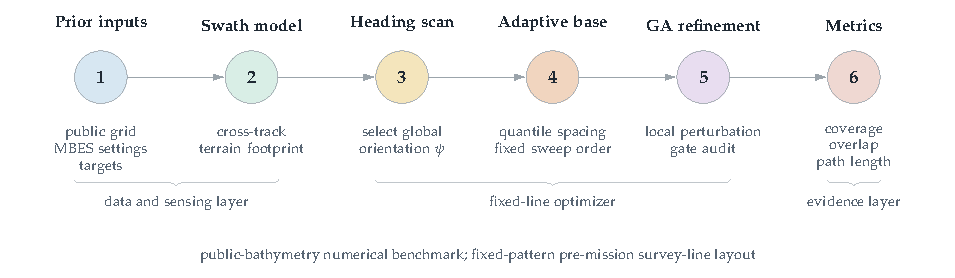
\includegraphics[width=\textwidth]{pic/method_pipeline.pdf}
	\iffalse
	\resizebox{\textwidth}{!}{%
	\begin{tikzpicture}[
		font=\sffamily,
		>=Latex,
		tag/.style={
			circle,
			draw=black!28,
			line width=0.22pt,
			minimum size=4.4mm,
			inner sep=0pt,
			font=\bfseries\tiny
		},
		stagebox/.style={
			rounded corners=1.45mm,
			draw=black!18,
			line width=0.22pt,
			fill=white,
			minimum width=29.2mm,
			minimum height=17.8mm,
			text width=25.8mm,
			align=left,
			inner sep=1.9mm
		},
		stephead/.style={
			font=\bfseries\scriptsize,
			text=black!86,
			align=left
		},
		stepbody/.style={
			font=\scriptsize,
			text=black!66,
			align=left
		},
		link/.style={
			-{Latex[length=1.75mm,width=1.1mm]},
			draw=black!34,
			line width=0.28pt
		},
		note/.style={
			rounded corners=1.1mm,
			draw=black!12,
			line width=0.18pt,
			fill=black!2,
			text=black!66,
			font=\scriptsize,
			align=left,
			inner sep=1.6mm,
			text width=65mm
		}
	]
		\node[stagebox] (s1) at (0,0) {};
		\node[stagebox] (s2) at (3.45,0) {};
		\node[stagebox] (s3) at (6.90,0) {};
		\node[stagebox] (s4) at (10.35,0) {};
		\node[stagebox] (s5) at (13.80,0) {};

		\foreach \a/\b in {s1/s2,s2/s3,s3/s4,s4/s5}
			\draw[link] ($(\a.east)+(0.05,0)$) -- ($(\b.west)+(-0.05,0)$);

		\node[tag,fill=cyan!12] at ($(s1.north west)+(0.44,-0.44)$) {1};
		\node[tag,fill=teal!10] at ($(s2.north west)+(0.44,-0.44)$) {2};
		\node[tag,fill=yellow!17] at ($(s3.north west)+(0.44,-0.44)$) {3};
		\node[tag,fill=violet!10] at ($(s4.north west)+(0.44,-0.44)$) {4};
		\node[tag,fill=blue!9] at ($(s5.north west)+(0.44,-0.44)$) {5};

		\node[stephead,anchor=north west] at ($(s1.north west)+(0.95,-0.35)$) {Inputs};
		\node[stepbody,anchor=north west] at ($(s1.north west)+(0.30,-1.07)$) {prior bathymetry\\MBES geometry\\coverage and overlap targets};

		\node[stephead,anchor=north west] at ($(s2.north west)+(0.95,-0.35)$) {Sensor--terrain model};
		\node[stepbody,anchor=north west] at ($(s2.north west)+(0.30,-1.07)$) {local swath \(W(x)\)\\port/starboard asymmetry\\predicted seafloor footprint};

		\node[stephead,anchor=north west] at ($(s3.north west)+(0.95,-0.35)$) {Orientation search};
		\node[stepbody,anchor=north west] at ($(s3.north west)+(0.30,-1.07)$) {greedy heading scan\\select global \(\psi\)\\fixed lawnmower frame};

		\node[stephead,anchor=north west] at ($(s4.north west)+(0.95,-0.35)$) {Line-layout refinement};
		\node[stepbody,anchor=north west] at ($(s4.north west)+(0.30,-1.07)$) {adaptive spacing\\GA over positions \(\mathbf{p}\)\\fixed sweep order};

		\node[stephead,anchor=north west] at ($(s5.north west)+(0.95,-0.35)$) {Evaluation};
		\node[stepbody,anchor=north west] at ($(s5.north west)+(0.30,-1.07)$) {path length and coverage\\excess overlap and feasibility\\50-seed repeatability};

		\node[note,anchor=north west] at (-1.52,-1.65) {Evidence: public GEBCO grids\\plus synthetic stress tests};
		\node[note,anchor=north east,align=right] at (15.33,-1.65) {Scope: offline public-data numerical benchmark\\prior-map planning under a fixed-pattern traversal};
	\end{tikzpicture}}
	\fi
	\caption{Method workflow for the proposed terrain-aware fixed-line MBES planner. A prior bathymetric surface and MBES configuration are converted into terrain-dependent swath predictions; a greedy search selects the global survey orientation \(\psi\); adaptive spacing and local GA refinement then place the parallel lines; and the final layout is scored by path length, coverage, excess overlap, feasibility, and seed repeatability.}
	\label{fig:method_pipeline}
\end{figure}

The method has two coupled layers. A sensor--terrain geometric model first converts a candidate line family into predicted coverage and overlap on the prior bathymetric surface. A bounded two-stage optimizer then searches the fixed sweep design space: a deterministic heading scan selects the global survey orientation, and a GA locally refines the sorted cross-track line positions while preserving the inspectable parallel-line traversal.

Efficient bathymetric coverage over irregular seabed requires an explicit mapping from each candidate line to the terrain region that can actually be observed. The constant-swath approximation used in many CPP formulations is adequate only when the bottom is close to planar. On more complex terrain, the effective footprint depends on slope, relief, and the relative orientation between the vehicle track and the local seabed surface. Consequently, uniform line spacing can produce substantial redundant overlap in some areas while still leaving under-covered regions elsewhere \cite{shi2020data,yordanova2020coverage,li2024multi}.

To avoid the under- and over-coverage induced by a fixed nominal spacing, coverage is evaluated from the local sensor--terrain geometry rather than from a prescribed constant swath width. Let \(\psi\) denote a candidate global line orientation and let \(s\) parameterize position along a survey line. For each sampled position \(s\), the MBES fan is analyzed in the cross-track plane orthogonal to the vehicle heading. The implementation uses the closed-form local planar approximation in Equations~\eqref{eq:depth}--\eqref{eq:swath}: the outer fan beams are intersected with the locally inclined cross-track bottom section to estimate a total effective swath width. It does not perform beam-by-beam acoustic ray tracing or return survey-grade port/starboard line products.

This local construction can be interpreted as yielding side-specific cross-track extents,
\[
w_{\mathrm{port}}(s,\psi)
\quad\text{and}\quad
w_{\mathrm{star}}(s,\psi),
\]
from which the effective local swath width is defined as
\[
w(s,\psi)=w_{\mathrm{port}}(s,\psi)+w_{\mathrm{star}}(s,\psi).
\]
The two-side decomposition matters because local relief can make the insonified footprint asymmetric. In the reported benchmark, however, those side contributions are collapsed into a total-width spacing proxy before raster evaluation. To make this simplification auditable, the reproducibility package includes a side-specific footprint validity audit that preserves separate port and starboard reach estimates for the same representative fixed-line layouts and compares the resulting coverage, overlap, cell-count disagreement, and \(C97/O3\) feasibility decisions against the manuscript proxy. A survey-grade extension should still preserve explicit port/starboard footprints together with roll/pitch/heave effects, sound-speed structure, and beam-level quality information.

Within the CPP formalism, this terrain-dependent sensing model defines the coverage operator used to score a candidate lawnmower layout. For each survey line, the operator maps the line and the prior bathymetric surface to a predicted covered seabed subset. Coverage completeness is then computed from the union of these subsets, while redundant sensing is summarized by the adjacent-spacing stress measure defined below. This representation links line placement directly to the objective terms introduced in the problem setting: reducing route length and excess overlap without allowing uncovered gaps.

Operationally, the reported evaluator is raster based and intentionally simpler than a hydrographic line-product pipeline. Candidate line families are transformed into a projected local grid, invalid or out-of-window cells are excluded, and each valid cell is tested by horizontal cell-center distance to the nearest planned line. A cell is counted as covered if that distance is no larger than one half of the local predicted total swath width after clipping to the declared evaluator limits. Coverage is therefore a horizontal grid-cell fraction over the valid target window, not a slope-area-weighted seabed-surface integral. The reported excess-overlap value is the area-averaged adjacent-spacing stress metric defined below; it is not an all-line intersection count, a beam-density map, or an IHO-quality sounding product.

The use of a geometry-aware operator is motivated by the same limitation that motivates the planning problem itself. Because MBES swath width changes with local slope and relief, a constant-spacing approximation can be inconsistent with the actual footprint implied by the terrain. Methods based on idealized fan-shaped or circular sensing abstractions do not capture this coupling between seafloor geometry and sonar footprint, and are therefore less suitable for evaluating fixed-track survey layouts when a prior terrain model is available \cite{xie2024three,mu2025coverage}. Likewise, recent adaptive-spacing studies support the need to vary spacing in nonuniform terrain rather than treating coverage width as constant \cite{zhang2022online,yan2024dual}.

In this work, the operator is used offline during mission design. The method therefore evaluates a nominal prior bathymetric model, nominal vehicle pose along each line, and declared sensor configuration. If the realized terrain differs from the prior map, if navigation error shifts the vehicle relative to the planned track, or if altitude deviations alter the effective footprint, then realized coverage can depart from the predicted coverage used by the optimizer. The model should therefore be read as a terrain-aware geometric swath approximation. It does not model beam-level bathymetric uncertainty, sound-speed refraction, roll/pitch/heave-dependent footprint deformation, closed-loop altitude control, or seabed backscatter quality. Predicted coverage is consequently a planning-layer metric rather than a hydrographic-quality assurance statement. We test part of this gap later with a Monte Carlo execution-uncertainty replay, while leaving online replanning, state-estimation feedback, and formal coverage assurance to execution-aware planners.

We model the MBES by its total opening angle $\varphi$ and evaluate candidate coverage in the vertical plane orthogonal to the survey heading. This construction isolates the cross-track geometry that determines swath width for a fixed lawnmower pattern. The reported benchmark is depth-referenced: it uses the public bathymetric depth at the survey line as the transducer-to-bottom range proxy, which is appropriate for a surface-referenced MBES geometry benchmark and for comparing fixed-line spacing on public gridded bathymetry. It is not an altitude-hold AUV footprint model. Because the public grids do not include vessel draft, sonar-head offset, tide, or heave, the benchmark sets transducer draft to zero relative to the gridded water surface, equivalently absorbing it into \(D_0\); a deployment with a known draft or sonar-head offset should replace \(D_0\) by \(D_0-z_T\) after tide/heave correction before applying the same evaluator and clipping rules. A low-altitude AUV implementation would replace the depth term below by vehicle altitude above bottom, \(h(s)\), and would add altitude-control, terrain-following, safety-clearance, and vehicle-dynamics constraints. Let $D_0$ be the depth at a reference point on the line, let $a$ denote the local seabed slope magnitude, and let $\beta$ denote the angle between the survey heading and the direction of steepest descent. Because along-track slope does not change the cross-track footprint in this local model, only the cross-track component of the terrain inclination is retained.

Define the effective cross-track inclination angle $a_1$ by projecting the local slope onto the direction normal to the survey line:
\begin{equation}
\tan a_1 = \tan a \cdot \cos(\beta - 90^{\circ}).
\end{equation}
Under the local planar approximation, the bathymetry in the cross-track section is then represented as a linear depth profile,
\begin{equation}
D(x) = D_0 - x \tan(a_1),
\label{eq:depth}
\end{equation}
where $x$ is the horizontal offset measured from the reference point in the direction perpendicular to the survey line. This approximation provides the terrain-dependent depth needed to evaluate how swath width changes with survey orientation and local seabed geometry.

The local swath width is computed from the same cross-track geometry. For a survey line at position $x$, the outer port and starboard beams leave the transducer at half-angle $\varphi/2$. When the seafloor is laterally inclined, these two beams intersect the bottom at different slant ranges, which makes the upslope and downslope contributions to the insonified strip unequal. The horizontal swath width is therefore
\begin{equation}
W(x) = \left( \frac{D(x) \sin(\varphi/2)}{\sin(90^{\circ} + a_1 - \varphi/2)} + \frac{D(x) \sin(\varphi/2)}{\sin(90^{\circ} - a_1 - \varphi/2)} \right) \cos(a_1).
\label{eq:swath}
\end{equation}
This expression explicitly captures the asymmetry induced by the local cross-track slope. When $a_1=0$, it simplifies to the flat-bottom relation $W(x)=2D(x)\tan(\varphi/2)$. The implementation applies the same bounded evaluator to every compared method: the two denominator terms in \eqref{eq:swath} are protected by a signed lower bound of \(10^{-3}\) in absolute value, non-finite width values are mapped to zero before clipping, and the final local total swath width is clipped to
\[
W_{\min}=30~\mathrm{m}, \qquad W_{\max}=1800~\mathrm{m}.
\]
No additional slope-class exclusion is used in the main benchmark; steep or near-singular cells therefore enter through this common denominator protection and width clipping. These constants prevent isolated cells from creating non-physical line spacing while keeping the same sensor--terrain approximation for Fixed-Spacing, Simple Greedy, Adaptive Spacing without GA, Fixed-Swath GA, and Full Geometry-Aware Hybrid GA. The model should consequently be interpreted as a controlled planning approximation rather than as beam-level acoustic ray tracing.
The upper cap \(W_{\max}=1800~\mathrm{m}\) is a declared benchmark range limit rather than an unconstrained physical swath claim. It prevents very deep GEBCO cells from producing unrealistically wide line spacing under the depth-referenced approximation. Because all methods are evaluated with the same cap, the reported differences should be interpreted as relative fixed-line layout improvements within this declared evaluator, not as absolute sonar-range predictions.

In the planner, \eqref{eq:depth}--\eqref{eq:swath} define the terrain-dependent sensing model used to score candidate line sets under the fixed lawnmower traversal. For each candidate orientation, the model is queried repeatedly to estimate admissible line spacing and the resulting overlap or under-coverage along neighboring lines. These quantities are then passed to the subsequent orientation search and line-placement optimization stages. The notation used in this model is summarized in Table~\ref{tab:table1}.

The model assumes that each local cross-track section can be approximated as planar. This approximation is appropriate for offline planning with a prior bathymetric surface, but its accuracy degrades where the terrain exhibits strong within-swath curvature, sharp ridges, or rapidly varying small-scale relief. In such regions, the predicted width should be interpreted as a local approximation rather than an exact footprint.

\begin{table}[!htbp]
	\centering
	\caption{Notation used by the terrain--sensor model and the adjacent-swath overlap calculation.}
	\label{tab:table1}
	\footnotesize
	\renewcommand{\arraystretch}{1.15}
	\begin{tabular}{lp{0.72\linewidth}}
		\toprule
		\textbf{Symbol} & \textbf{Definition} \\
		\midrule
		$D_0$ & Depth-referenced transducer-to-bottom range proxy at the local reference point (m) \\
		$a$ & Dominant seafloor slope angle relative to the horizontal \\
		$\beta$ & Angle between the survey-track direction and the direction of steepest descent \\
		$a_1$ & Effective cross-track slope angle in the plane normal to the survey track \\
		$x$ & Horizontal distance from the reference point measured in the cross-track direction (m) \\
		$D(x)$ & Depth-referenced range proxy at position $x$ (m); replace by altitude \(h(x)\) for low-altitude AUV modeling \\
		$\psi$ & Global survey-line orientation ($^\circ$) \\
		$\varphi$ & Total multibeam opening angle ($^\circ$) \\
		$W(x)$ & Predicted swath width at position $x$ (m) \\
		$d$ & Spacing between adjacent survey lines (m) \\
		$\eta$ & Overlap ratio between adjacent swaths \\
		\bottomrule
	\end{tabular}
\end{table}

We formulate offline survey design as a search over the global line orientation $\psi$ and the sorted cross-track line positions $\mathbf{p}=[p_1,\ldots,p_N]$ of a fixed lawnmower pattern. Given $(\psi,\mathbf{p})$, the induced plan consists of $N$ parallel survey lines traversed in alternating directions. The geometric route cost is the total traversal length
\begin{equation}
L(\psi,\mathbf{p})
=
\sum_{i=1}^{N} \ell_i
+
\sum_{i=1}^{N-1} c_{i,i+1},
\end{equation}
where $\ell_i$ is the in-region length of line $i$ and $c_{i,i+1}$ is the transition distance between consecutive lines under the prescribed sweep order. This objective reflects the two dominant contributors to mission effort in the present benchmark: productive survey distance along the lines and the regular turn-to-turn transit imposed by the parallel-line layout. The objective optimizes line spacing and cross-track placement rather than vehicle dynamics. Because the output remains a fixed parallel-line family, the line-change segments can be smoothed after planning with standard Dubins, clothoid, or spline transitions. A turning-aware post-evaluation can be written as \(L_R(\psi,\mathbf{p})=L(\psi,\mathbf{p})+(N-1)\pi R_{\min}\) for a conservative semicircular line-change penalty, and a future execution-aware version can place \(R_{\min}\), turn-time, or curvature penalties directly in the GA fitness.

Coverage is evaluated from the union of line-specific footprints predicted by the sensor--terrain model. Let $\Omega$ denote the target survey region and let $\mathcal{F}_i$ be the predicted footprint of line $i$. The predicted coverage rate is
\begin{equation}
CR(\psi,\mathbf{p})
=
\frac{\left|\Omega \cap \bigcup_{i=1}^{N}\mathcal{F}_i\right|}{|\Omega|}\times 100\%.
\end{equation}
The evaluator rasterizes line footprints on the projected grid. A cell is counted as covered when its cross-track distance to at least one line is no greater than one half of the local predicted swath width; the reported coverage is the fraction of valid cells covered at least once. The excess-overlap diagnostic is a mean adjacent-spacing stress measure rather than a hydrographic line-product quality metric. The local overlap ratio between adjacent lines is defined as
\begin{equation}
\eta_i(x)=1-\frac{d_i}{W_i(x)},
\end{equation}
where $d_i=p_{i+1}-p_i$ and $W_i(x)$ is the effective swath width available at location $x$ for that adjacent-line pair. This approximation uses the local total swath width rather than a full side-specific port/starboard intersection model; it is adequate for the benchmark's spacing-regime comparison, but a survey-grade implementation should compute overlap from side-specific beam footprints and all-line intersections. Rather than enforcing a pointwise hard band everywhere, the implementation reports only the mean excess-overlap violation above the 20 percent ceiling,
\begin{equation}
O_{\mathrm{ex}}(\psi,\mathbf{p})
=
\frac{1}{|\Omega|}\int_{\Omega}\max\!\left(\eta(x)-0.20,\,0\right)\,d\Omega \times 100\%.
\end{equation}
The target-overlap design margin is 15 percent, while the reported feasibility test accepts a plan only if
\begin{equation}
CR(\psi,\mathbf{p}) \ge 97.0\%, \qquad O_{\mathrm{ex}}(\psi,\mathbf{p}) \le 3.0\%.
\end{equation}
This distinction affects how the benchmark should be read. The 10--20 percent overlap interval is the design intent used when constructing candidate line families, whereas the reported acceptance rule is expressed through domain-level predicted coverage and mean excess-overlap violation. The 97 percent coverage and 3 percent mean-excess-overlap gates are benchmark thresholds chosen to compare methods under a common numerical evaluator; stricter hydrographic or project-specific thresholds would need to be declared and re-evaluated before deployment.

The overlap margin, coverage gate, excess-overlap gate, and swath-width cap are benchmark design choices rather than hydrographic standards. IHO hydrographic guidance treats survey line spacing as dependent on survey requirements, range scale, depth, and required overlap, and its MBES guidance notes that swath-width variation with depth can justify splitting an area into subsections with different spacing \cite{iho_c13}. NOAA's HSSD similarly places crosslines, overlap, and swath acquisition inside project specifications and quality checks rather than a single universal overlap constant \cite{noaa_hssd2025}. The AusSeabed Australian Multibeam Guidelines also frame multibeam acquisition around pre-survey planning, calibration, acquisition, processing, and reporting procedures rather than a fixed numerical spacing rule \cite{ausseabed2020guidelines}. The present \(15\%\) design margin, \(20\%\) ceiling, \(C97/O3\) acceptance gate, and \(W_{\max}=1800\)~m cap therefore define a reproducible numerical benchmark. Table~\ref{tab:parameter_rationale} consolidates these choices, their rationale, and the diagnostics used to audit them.

\begin{table}[!htbp]
	\centering
	\caption{Benchmark-parameter rationale and associated robustness checks. The settings define the numerical planning benchmark used for method comparison; they are not presented as hydrographic survey-order requirements.}
	\label{tab:parameter_rationale}
	\scriptsize
	\renewcommand{\arraystretch}{1.10}
	\setlength{\tabcolsep}{3.0pt}
	\begin{tabular}{@{}>{\raggedright\arraybackslash}p{0.19\linewidth}>{\raggedright\arraybackslash}p{0.18\linewidth}>{\raggedright\arraybackslash}p{0.34\linewidth}>{\raggedright\arraybackslash}p{0.20\linewidth}@{}}
		\toprule[1bp]
		\textbf{Parameter} & \textbf{Default} & \textbf{Rationale} & \textbf{Audit in this study} \\
		\midrule[1bp]
		Target overlap margin & \(\eta_{\mathrm{tar}}=15\%\) & Planning margin inside the declared 10--20\% design band; used to generate candidate spacing rather than to certify line products. & Target-overlap diagnostic at 10\%, 15\%, and 20\%. \\
		Excess-overlap ceiling & \(20\%\) local adjacent-spacing ceiling & Separates intended overlap from redundant overlap under the adjacent-line spacing proxy. & Threshold/local-failure audit with 1--5\% mean-excess-overlap gates and cellwise tails. \\
		Default feasibility gate & \(C97/O3\) & Common numerical acceptance screen for comparing fixed-line layouts while keeping stricter tail checks separate. & \(C99/O2\), \(C99.5/O2\), largest-gap, and p95/p99 cellwise diagnostics. \\
		Swath-width clipping & \(W_{\min}=30\)~m, \(W_{\max}=1800\)~m & Prevents near-singular or very deep cells from producing non-physical spacing under the depth-referenced approximation. & \(W_{\max}=1200/1800/2400\)~m submission-boundary diagnostic. \\
		Heading grid & \(15^{\circ}\) main scan & Reproducible global orientation search for an inspectable fixed-line family. & \(5^{\circ}\) deterministic heading-resolution audit. \\
		Score weights & 80 km per coverage pp; 3 km per overlap pp & Prioritizes coverage-gate satisfaction before route shortening in a shared scalar score. & \(3\times3\) coverage/overlap penalty-weight diagnostic. \\
		GA budget & 10 individuals, 10 generations & Local cleanup around a deterministic heading and adaptive-spacing base, not blind global CPP search. & 50-seed repeatability, GA-gate diagnostic, and stride-3/full-grid surrogate audit. \\
		\bottomrule[1bp]
	\end{tabular}
\end{table}

These settings are exposed to sensitivity and threshold diagnostics instead of being presented as survey-order requirements.

Because mean coverage and mean excess-overlap gates can hide local failures, the reproducibility package also reports a threshold and local-failure diagnostic. That diagnostic re-evaluates the two primary GEBCO scenes and the USGS high-complexity crop under coverage thresholds of 95, 97, 98, 99, and 99.5 percent; mean-excess-overlap gates of 1, 2, 3, and 5 percent; largest connected uncovered-patch size; and the 95th- and 99th-percentile cellwise excess-overlap tails. These diagnostics are not used to change the main benchmark gate; they audit how much margin remains if a stricter project-specific rule is imposed.

Candidate plans are ranked by the same scalar score used in the implementation,
\begin{equation}
S(\psi,\mathbf{p})
=
L(\psi,\mathbf{p})
+ 80\max\!\left(97.0-CR(\psi,\mathbf{p}),\,0\right)
+ 3\,O_{\mathrm{ex}}(\psi,\mathbf{p}),
\label{eq:plan_score}
\end{equation}
where \(L\) is measured in kilometers in the reported implementation. Thus the 80 coefficient has units of km per percentage point of coverage shortfall, whereas the overlap coefficient has units of km per percentage point of mean excess-overlap violation. These weights are benchmark weights rather than universal engineering constants. They intentionally prioritize satisfying the coverage gate before shortening the route; a deployment planner could instead use a nondimensional multi-objective score or lexicographic ordering. The 97 percent coverage value is likewise a benchmark acceptance threshold used to compare all methods under the same evaluator; it is not presented as a hydrographic survey standard or a field-coverage guarantee. This formulation targets offline survey design with a prior bathymetric model. If the realized seabed or executed trajectory deviates materially from the assumed prior and nominal line tracking, then actual overlap and coverage can depart from the predicted values used by the optimizer.

The implemented benchmark compares five method variants built on the same score and sensor--terrain evaluator: Fixed-Spacing, Simple Greedy, Adaptive Spacing without GA, Fixed-Swath GA, and Full Geometry-Aware Hybrid GA. The variants differ only in how the orientation and line positions are generated.

\paragraph{Discrete orientation scan and constant-spacing baseline}
The first deterministic component scans candidate headings
\[
\psi \in \{0^{\circ},15^{\circ},\ldots,165^{\circ}\}.
\]
For each heading, a constant-spacing baseline is constructed from the scene-wide swath-width distribution. Let $\widetilde{W}_{q}(\psi)$ denote the $q$-quantile of the terrain-aware swath widths evaluated under heading $\psi$. For each
\[
q \in \{0.15,0.20,0.25,0.30,0.35,0.40,0.45,0.50\},
\]
a constant inter-line spacing is proposed as
\begin{equation}
d_q(\psi)=\widetilde{W}_{q}(\psi)\left(1-\eta_{\mathrm{tar}}\right),
\qquad \eta_{\mathrm{tar}}=0.15.
\end{equation}
The resulting parallel-line family is scored by \eqref{eq:plan_score}, and the best candidate over all headings and constant-spacing quantiles defines the Simple Greedy baseline. Fixed-Spacing uses the same constant-spacing construction at the reference heading $\psi=0^{\circ}$ only. This scan is not a proof of global optimality, but it is fully reproducible and provides a stable geometry-aware orientation prior for the later refinements.

Because the public-scene route gains are deliberately reported at sub-percent scale, the reproducibility package also includes a heading-resolution diagnostic that reruns the deterministic Simple Greedy and Adaptive Spacing bases with a finer \(5^{\circ}\) heading grid. The \(15^{\circ}\) grid remains the declared main benchmark setting, whereas the \(5^{\circ}\) rerun audits whether heading quantization is large enough to change the interpretation. Hybrid GA is not rerun as a separate optimizer in this diagnostic because it inherits the deterministic adaptive heading and line-count base.

\paragraph{Adaptive spacing without GA}
The second deterministic component replaces a single scene-wide spacing by a cross-track spacing profile derived from local swath statistics. For each candidate heading, the rotated cross-track coordinate $v$ is divided into 160 bins. In each bin, the planner computes a swath-profile quantile
\[
\widehat{W}_{q}(v), \qquad q \in \{0.20,0.25,0.30,0.35\},
\]
and interpolates it over the full cross-track extent. Starting from the first admissible line position, the line family is then generated recursively by
\begin{equation}
p_{k+1}=p_k+\widehat{W}_{q}(p_k)\left(1-\eta_{\mathrm{tar}}\right).
\label{eq:adaptive_spacing}
\end{equation}
The best heading/profile pair under \eqref{eq:plan_score} defines the Adaptive Spacing without GA baseline. This step is crucial for interpreting the results because it isolates how much benefit comes from terrain-aware spacing itself before any stochastic search is added.

\paragraph{GA refinement of line positions}
The two GA variants keep the heading fixed and refine only the sorted cross-track positions $\mathbf{p}$. Fixed-Swath GA starts from the best constant-spacing candidate returned by the discrete orientation scan, whereas Full Geometry-Aware Hybrid GA starts from the adaptive-spacing baseline. In both cases, the number of lines is inherited from the deterministic base layout and remains fixed within a run.

The GA is real coded. The initial population contains the base layout plus nine jittered variants, where each gene is perturbed by zero-mean Gaussian noise with standard deviation 0.10 times the nominal median spacing. Fitness is evaluated on a stride-3 subsampled grid for speed, while the selected layout is always rescored on the full evaluator grid before any manuscript metric is reported. A supplemental surrogate audit samples local perturbations around the deterministic adaptive layout and compares the stride-3 GA-fitness ranking with full-grid rescoring, so the use of the subsampled fitness is treated as an auditable acceleration rather than as an unchecked replacement evaluator. Tournament selection uses three candidates, arithmetic crossover draws $\alpha \sim \mathcal{U}(0.30,0.70)$ and forms the child as $\alpha \mathbf{p}^{(a)} + (1-\alpha)\mathbf{p}^{(b)}$, and mutation perturbs each gene independently with probability 0.30 using Gaussian noise with standard deviation 0.05 times the nominal spacing. The implementation uses elitism but does not impose a Pareto acceptance gate against the deterministic adaptive baseline in the main benchmark; consequently, a GA-refined seed can trade a very small path reduction for slightly lower predicted coverage or slightly higher residual overlap. This behavior is reported explicitly in the ablation and is one reason the paper treats GA as local refinement rather than as the main contribution.

The small GA budget is intentional. The discrete heading scan and adaptive-spacing stage already provide a strong base layout, so the GA is not a blind global search over route topology; it only tests small local perturbations to sorted cross-track line positions. A population of 10 and 10 generations therefore functions as a rapid cleanup audit around the deterministic baseline, not as a claim that a very small GA can solve arbitrary CPP globally. In the reported main benchmark, Full Geometry-Aware Hybrid GA planning time ranges from 0.32 to 0.94~s across the five main scenes, with public-scene means of 0.92~s on GEBCO Cascadia and 0.56~s on GEBCO Monterey. These timings support its role as an inexpensive offline refinement layer.

To make the boundary auditable, the submission-boundary diagnostic also reports a conservative operational gate: accept a raw Hybrid GA seed only when it is feasible, no worse than Adaptive Spacing without GA by 0.05 percentage points in coverage and mean excess overlap, and no longer in path length; otherwise the selected layout falls back to the deterministic adaptive layout. This gate is not used to alter the reported main benchmark means. It is a practical-significance check on whether stochastic cleanup should be deployed. A spacing-regularity penalty,
\begin{equation}
P_{\mathrm{sep}}(\mathbf{p})
=
0.04\sum_{i=1}^{N-1}\max\!\left(0,\,0.25\,\bar{d}-\left(p_{i+1}-p_i\right)\right),
\end{equation}
is added when adjacent lines collapse below one quarter of the nominal spacing $\bar{d}$. The final GA fitness is therefore
\begin{equation}
S_{\mathrm{GA}}(\psi,\mathbf{p})=S(\psi,\mathbf{p})+P_{\mathrm{sep}}(\mathbf{p}).
\end{equation}
Each run uses 10 generations, population size 10, and elitism, so the best individual found so far is copied directly into the next generation. The output is a fixed-pattern line family with the same global heading as the base layout.

The resulting optimizer is intentionally narrow: it tests whether prior-bathymetry-guided spacing, with optional local position cleanup, improves track length and overlap discipline relative to uniform spacing under the same fixed traversal, while maintaining predicted coverage. Route-order optimization, online replanning, and closed-loop adaptation to prior-map mismatch are therefore downstream extensions rather than hidden components of the present method.

For reproducibility, each benchmark run follows the same sequence: compute terrain-aware swath statistics for every candidate heading, generate the best deterministic baseline under \eqref{eq:plan_score}, inherit that baseline into the relevant GA variant when stochastic refinement is enabled, and finally rescore the selected layout on the full evaluator grid before reporting path length, predicted coverage, excess overlap, planning time, and feasibility. Table~\ref{tab:planner_settings} consolidates the fixed implementation settings used by the planner in the main benchmark.

\begin{table}[!htbp]
	\centering
	\caption{Fixed implementation settings used by the planner in the main benchmark. Sensitivity diagnostics change only the declared setting under test unless noted otherwise.}
	\label{tab:planner_settings}
	\scriptsize
	\renewcommand{\arraystretch}{1.12}
	\setlength{\tabcolsep}{3.8pt}
	\begin{tabular}{@{}p{0.31\linewidth}p{0.61\linewidth}@{}}
		\toprule[1bp]
		\textbf{Component} & \textbf{Setting} \\
		\midrule[1bp]
		Heading scan & $\psi \in \{0^{\circ},15^{\circ},\ldots,165^{\circ}\}$ \\
		Constant-spacing candidates & $q \in \{0.15,0.20,0.25,0.30,0.35,0.40,0.45,0.50\}$ with $d_q(\psi)=\widetilde{W}_{q}(\psi)(1-\eta_{\mathrm{tar}})$ \\
		Adaptive profile candidates & $q \in \{0.20,0.25,0.30,0.35\}$ over 160 cross-track bins, followed by the recursive update in \eqref{eq:adaptive_spacing} \\
		Target overlap margin & $\eta_{\mathrm{tar}}=0.15$ \\
		Acceptance rule & $CR(\psi,\mathbf{p}) \ge 97.0\%$ and $O_{\mathrm{ex}}(\psi,\mathbf{p}) \le 3.0\%$ \\
		Base GA population & Deterministic base layout plus nine jittered layouts \\
		Initialization jitter & Zero-mean Gaussian noise with standard deviation $0.10$ times the nominal median spacing \\
		Selection and crossover & Tournament size 3; arithmetic crossover with $\alpha \sim \mathcal{U}(0.30,0.70)$ \\
		Mutation & Per-gene probability 0.30; Gaussian perturbation with standard deviation $0.05$ times the nominal spacing \\
		Spacing-regularity penalty & Activated when adjacent lines fall below $0.25\,\bar d$ \\
		GA schedule & 10 generations, population size 10, elitist carryover of the current best individual; used as local refinement after deterministic orientation and spacing initialization \\
		Fitness evaluation & Stride-3 subsampled grid during GA; full evaluator grid for the reported metrics \\
		Stochastic repeats & 50 seeds for Fixed-Swath GA and Full Geometry-Aware Hybrid GA in the main benchmark \\
		\bottomrule[1bp]
	\end{tabular}
\end{table}

\subsection{Experimental evaluation protocol}
The numerical evaluation uses the benchmark suite reported in this study. The reproducible global-prior benchmark consists of two public GEBCO~2025 bathymetry subsets, GEBCO Cascadia Margin and GEBCO Monterey Canyon. Because GEBCO is a heterogeneous global information product, these scenes are treated as public-prior line-layout tests rather than as survey-grade validation. The strongest high-resolution transfer check uses three crops from the USGS Southern Cascadia 30~m multibeam-derived public grid, and the coarse-prior/fine-grid replay further tests whether a line family planned on coarsened priors survives evaluation on a finer public grid. The secondary synthetic set consists of Flat Seafloor, Uniform Slope, and Complex Terrain, which isolate mechanisms and stress-test the fixed-heading parallel-line assumption. To reduce scene-selection risk without redefining the benchmark, a supplemental four-window GEBCO expansion further probes Mariana Trench, Puerto Rico Trench, Mid-Atlantic Ridge, and Hawaii Ridge subsets with the same evaluator and 50 Hybrid GA seeds.

Five methods are compared under the same sensor--terrain evaluator: Fixed-Spacing, Simple Greedy, Adaptive Spacing without GA, Fixed-Swath GA, and Full Geometry-Aware Hybrid GA. Fixed-Spacing is the reference \(0^{\circ}\) constant-spacing lawnmower used to expose the cost of not adapting the line family. Simple Greedy is the fairness baseline for heading rotation: it scans the same candidate headings as the proposed method, but keeps constant spacing within each heading. Adaptive Spacing without GA then adds the terrain-dependent quantile profile without stochastic refinement, so the ablation separates reference-heading choice, best constant-spacing heading, adaptive spacing, and local GA perturbation. The reported metrics are total path length, predicted coverage, excess overlap above the prescribed ceiling of 20 percent, planning time, and a feasibility flag. Lower values are preferred for path length, excess overlap, and computation time, whereas higher values are preferred for predicted coverage. The benchmark uses a $97.0\%$ coverage target, a 15 percent target-overlap design margin, a 3.0 percent mean excess-overlap feasibility ceiling, a $120^{\circ}$ MBES opening angle, candidate headings from $0^{\circ}$ to $165^{\circ}$ in $15^{\circ}$ increments, 10 GA generations, a population size of 10, and 50 seeds for stochastic GA methods. Fixed-Spacing, Simple Greedy, and Adaptive Spacing without GA are deterministic in this implementation. The GEBCO windows are regional rather than sortie-scale, spanning roughly $128 \times 178$~km and $90 \times 111$~km after cropping. Their absolute route lengths should therefore be interpreted as large-area benchmark totals, not as single-sortie vehicle budgets. At a nominal 1.5~m/s speed, the reported GEBCO Hybrid GA route totals would correspond to approximately 116~days for Cascadia and 51~days for Monterey, which is why these scenes are used as reproducible regional geometry benchmarks rather than executable single-vehicle missions. The USGS crops are much closer to sortie-scale fixed-line geometry tests, with reported paths of roughly 52--97~km depending on crop and method.

The comparator set is chosen to isolate fixed-pattern line-layout effects rather than to rank all underwater CPP algorithms. Online bathymetric SLAM planners, cooperative multi-AUV planners, and energy-aware vehicle-dynamics planners solve broader problems with additional objectives, route topologies, or information states. Directly comparing against them would mix terrain-aware MBES spacing with route sequencing, localization, vehicle allocation, or control design. The baselines here instead form a controlled ladder inside the same fixed-pattern family: constant spacing, greedy spacing, adaptive spacing without stochastic refinement, GA under a fixed swath abstraction, and the full geometry-aware hybrid planner. This makes the ablation interpretable: any improvement can be attributed to terrain-dependent spacing, heading selection, or GA refinement rather than to a change in the mission-planning problem itself. To reduce the separate risk that this ladder is too internal, a supplemental external heuristic audit also evaluates three deterministic survey-layout rules--minimum cross-track span, contour-parallel fixed-width lines, and geometry-shortest fixed-width lines--on the same nine public-grid windows and under the same evaluator. These heuristics are external-style layout checks rather than full reproductions of field-ready CPP systems.

Table~\ref{tab:public_provenance} records the provenance of the GEBCO public-prior benchmark set. Both public scenes are GEBCO~2025 grid subsets with complete valid-cell coverage in the saved manifests. They are therefore publicly released gridded bathymetry inputs to a numerical planner, not AUV mission logs, raw MBES returns, or field-executed survey tracks.

\begin{table}[!htbp]
	\centering
		\caption{Public GEBCO bathymetry subsets used as the reproducible public-prior benchmark. Bounds are geographic crop limits in EPSG:4326; extents are computed from the locally projected evaluator grids used in this study. The listed grid resolutions are projected cell sizes after crop-and-project preprocessing, not the native angular spacing of the global GEBCO product.}
	\label{tab:public_provenance}
	\scriptsize
	\renewcommand{\arraystretch}{1.12}
	\setlength{\tabcolsep}{2.2pt}
	\begin{tabular}{@{}p{0.17\linewidth}p{0.22\linewidth}p{0.14\linewidth}p{0.12\linewidth}p{0.12\linewidth}p{0.05\linewidth}@{}}
		\toprule[1bp]
		\textbf{Scene} & \textbf{Crop bounds} & \textbf{Extent} & \textbf{Grid resolution} & \textbf{Depth range} & \textbf{Valid} \\
		\midrule[1bp]
		GEBCO Cascadia Margin & lon $-126.8$ to $-125.2$; lat $43.2$ to $44.8$ & $128.1 \times 178.1$ km & 1195.383 m & 1009--3101 m & 1.0 \\
		GEBCO Monterey Canyon & lon $-123.3$ to $-122.3$; lat $35.3$ to $36.3$ & $90.3 \times 111.3$ km & 758.720 m & 892--3982 m & 1.0 \\
		\bottomrule[1bp]
	\end{tabular}
\end{table}

The use of GEBCO also imposes a data-level boundary. The official GEBCO documentation describes the GEBCO~2025 Grid as a global terrain model and an information product derived from heterogeneous source data and interpolation; it is accompanied by a Type Identifier (TID) grid that records source-data categories for grid cells \cite{gebco2025grid}. To make that boundary explicit, Table~\ref{tab:gebco_tid_audit} reports a TID audit downloaded from the GEBCO subset API for the two primary windows. The values show that both windows are dominated by TID~11 cells, while still containing smaller fractions of TID~10, TID~40, and TID~44 cells. These TID values are official provenance layers, not inferred labels. When an official provenance layer is unavailable, the planner can still construct derived planning layers from the bathymetry itself--for example slope, local relief, curvature, swath-risk, or source-confidence masks informed by available provenance checks. Those layers may be useful for weighting or auditing a planner, but they must be reported as derived planning products rather than as measured source categories; in particular, missing TID/source fractions should not be fabricated. The present benchmark therefore uses the elevation subsets after crop-and-project preprocessing and reports the TID audit, but it does not optimize line placement with TID values or source-specific uncertainty. The public scenes should be read as external public-grid benchmarks for offline line-layout evaluation, not as survey-grade terrain products or safety-of-navigation inputs.

\begin{table}[!htbp]
	\centering
	\caption{GEBCO~2025 Type Identifier (TID) audit for the two primary public-prior scenes. TID definitions follow GEBCO's published coding \cite{gebco_tid_grid}: 10 denotes singlebeam sounding cells, 11 denotes multibeam sounding cells, 40 denotes satellite-gravity-guided predicted cells, and 44 denotes sounding-constrained cells in a gridded data set with satellite-gravity-guided interpolation. Percentages are cell fractions in the downloaded TID subset and are used as provenance evidence; the planner itself is not TID-weighted.}
	\label{tab:gebco_tid_audit}
	\scriptsize
	\renewcommand{\arraystretch}{1.10}
	\setlength{\tabcolsep}{4.2pt}
	\begin{tabular}{@{}lrrrr@{}}
		\toprule[1bp]
		\textbf{Scene} & \textbf{TID 10} & \textbf{TID 11} & \textbf{TID 40} & \textbf{TID 44} \\
		\midrule[1bp]
		GEBCO Cascadia Margin & 0.41\% & 91.05\% & 5.44\% & 3.10\% \\
		GEBCO Monterey Canyon & 0.02\% & 95.47\% & 2.92\% & 1.58\% \\
		\bottomrule[1bp]
	\end{tabular}
\end{table}

In addition to the main benchmark suite, we run lightweight public-scene sensitivity diagnostics on declared sensor and planning inputs. The MBES-opening diagnostic reruns Fixed-Spacing, Adaptive Spacing without GA, and Full Geometry-Aware Hybrid GA on the two GEBCO scenes with opening angles of \(100^{\circ}\), \(110^{\circ}\), \(120^{\circ}\), and \(130^{\circ}\). The target-overlap diagnostic reruns the same methods at margins of 10\%, 15\%, and 20\%, using the reported \(120^{\circ}\) MBES opening angle. The resolution diagnostic reruns the same methods on the native public grids and on \(2\times\) and \(3\times\) strided downsampled versions. The supplementary prior-map diagnostics rerun the public scenes under uniform depth biases of \(\pm 150\)~m and relief-scale factors of 0.7, 1.0, and 1.3, and a penalty-weight diagnostic reruns them across a \(3\times3\) coverage/overlap objective-weight grid. A separate supplemental GEBCO four-window expansion checks whether the same low-overlap public-scene pattern persists on four additional public bathymetry windows. A separate USGS coarse-prior/fine-grid replay plans the selected public crops on 120, 300, 600, and 900~m priors and then rescores the same line families on a finer public grid without re-optimization. A structured prior-error replay then plans on priors with low-frequency correlated bias, slope-amplified error, and localized canyon-wall perturbations before replaying the selected line families on the truth grid. An uncertainty-aware margin replay sweeps declared target-overlap and swath-quantile margins, accepts GA cleanup only when nominal coverage and overlap gates are preserved, and selects a margin by replaying the declared execution-error envelope before final 300-trial evaluation. Finally, a current-drift replay converts mild, cross, and adverse current proxies into residual cross-track line drift, heading perturbation, and terrain-coupled footprint shrinkage before recomputing the same coverage and overlap metrics. The hybrid planner is summarized over seeds 0--19 for the public-scene sensitivity diagnostics, coarse-prior diagnostics, and structured prior-error replay, and over seeds 0--49 for the supplemental GEBCO expansion and USGS public-grid extension. These runs are not treated as replacements for the main 50-seed benchmark; they are used only to test whether the public-scene conclusions are fragile to small declared changes in sensor aperture, spacing margin, public-grid resolution, simple global prior-map perturbations, spatially structured map error, objective weighting, scene selection, controlled prior-resolution mismatch, declared execution-envelope margin selection, or current-drift stress.

A submission-boundary diagnostic adds two final checks requested before journal upload. First, it reruns Fixed-Spacing, Simple Greedy, Adaptive Spacing without GA, and Full Geometry-Aware Hybrid GA on the two primary GEBCO scenes and the USGS high-complexity crop with \(W_{\max}=1200\), 1800, and 2400~m, while keeping the same \(W_{\min}=30\)~m and evaluator rules. Second, at the reported \(W_{\max}=1800\)~m, it compares 20 raw Hybrid GA seeds against the deterministic Adaptive Spacing layout using the conservative gate defined above. These outputs are treated as boundary and practical-significance diagnostics, not as replacements for the main benchmark.

The structured prior-error replay is distinct from the execution-noise replay. It changes the map available at planning time, not the line execution after planning. The correlated-bias setting uses a low-frequency prior-depth error field with a 35~m RMS scale. The slope-amplified setting combines correlated error with higher variance on high-gradient seabed cells. The localized canyon-wall setting adds two compact high-slope perturbations to represent the kind of prior mismatch that can occur near canyon walls or steep relief. Each perturbed prior is planned independently, and the resulting line family is replayed on the unperturbed truth grid with the same coverage and overlap evaluator. The design is a controlled stress replay rather than a probabilistic seafloor-error model: it asks whether line placement remains safe when the bathymetric prior is spatially wrong rather than merely globally shifted.

We also add a post-planning execution-uncertainty replay on the two public GEBCO layouts. The replay does not re-optimize the line family. Instead, it perturbs the already selected Fixed-Spacing, Adaptive Spacing without GA, and representative Hybrid GA layouts, then recomputes predicted coverage and excess overlap on the same public-grid evaluator. The moderate-noise setting uses independent line-level cross-track perturbations with standard deviation \(0.05\bar d\), a global cross-track offset with standard deviation \(0.02\bar d\), heading noise with standard deviation \(0.5^{\circ}\), a 3 percent global footprint-scale perturbation, and 2 percent spatially correlated local footprint-scale noise, where \(\bar d\) is the median planned inter-line spacing. The strong-noise setting doubles these levels to \(0.10\bar d\), \(0.04\bar d\), \(1.0^{\circ}\), 6 percent, and 4 percent. Each non-nominal setting uses 300 Monte Carlo trials per scene and method. This experiment is a numerical uncertainty replay, not a substitute for mission logs, but it directly tests whether the selected public layouts retain coverage and overlap margin under plausible post-planning perturbations.

\section{Results}
\label{sec:results}
The benchmark suite is organized around an evidential hierarchy rather than a single aggregate score. Two public GEBCO~2025 bathymetry subsets \cite{gebco2025grid}, GEBCO Cascadia Margin and GEBCO Monterey Canyon, provide the reproducible global-prior benchmark for the offline planner. The USGS Southern Cascadia 30~m multibeam-derived crops and the coarse-prior/fine-grid replay provide the higher-resolution public-grid transfer evidence. Three synthetic terrains isolate flat, sloped, and strongly heterogeneous seafloor mechanisms, and the remaining diagnostics test transfer, prior fidelity, and execution margin without merging those checks into the GEBCO public-prior averages. Only outputs generated from the reported terrain-aware MBES evaluator are included.

The same metrics and acceptance criteria defined in the protocol are used throughout this section. Coverage values are predicted coverage rates under the reported sensor--terrain model, not measured field coverage. The GEBCO windows are regional rather than sortie-scale, so their absolute route-length values should be interpreted as benchmark totals rather than as single-mission vehicle budgets.

Table~\ref{tab:evidence_map} organizes the Results section by evidential role. GEBCO public-prior figures and tables establish reproducibility on globally available gridded bathymetry; USGS and coarse-prior replay cases provide stronger high-resolution transfer evidence; synthetic cases explain the overlap regime in which the method matters; ablation, repeatability, PSO, and external heuristic audits separate adaptive spacing from GA cleanup and from simpler survey-layout rules; and robustness replays define what the fixed-line geometry can and cannot support before mission-log or controller-level validation is available. A supplemental four-window GEBCO expansion is reported as a scene-selection risk check rather than as a replacement for the reported GEBCO pair.

Table~\ref{tab:evidence_map} gives a compact evidence map for the Results section. The table is intentionally shorter than a full figure-by-figure roadmap: it identifies the evidential role of each result block while keeping detailed diagnostic matrices in the reproducibility package when they are secondary to the main claim.

\begin{table}[!htbp]
	\centering
	\caption{Compact evidence map for the Results section. Each row states the role of a result block, the evidence used, the claim supported, and the boundary that prevents over-interpretation.}
	\label{tab:evidence_map}
	\scriptsize
	\renewcommand{\arraystretch}{1.08}
	\setlength{\tabcolsep}{3.0pt}
	\begin{tabular}{@{}>{\raggedright\arraybackslash}p{0.18\linewidth}>{\raggedright\arraybackslash}p{0.25\linewidth}>{\raggedright\arraybackslash}p{0.31\linewidth}>{\raggedright\arraybackslash}p{0.13\linewidth}@{}}
		\toprule[1bp]
		\textbf{Role} & \textbf{Evidence used} & \textbf{Supported finding} & \textbf{Boundary} \\
		\midrule[1bp]
		Public-prior benchmark & GEBCO Cascadia and Monterey scene cards plus Table~\ref{tab:table2}. & Terrain-aware spacing reaches 98.99--99.55 percent predicted coverage, reduces mean excess-overlap violation from about 0.81 percent to 0.113 percent, and shortens mean path length by 0.75 percent. & Public prior-grid evidence, not field validation. \\
		High-resolution public-grid transfer & USGS 30~m extension and coarse-prior/fine-grid replay. & The high-complexity USGS crop exposes the strongest practical effect: Fixed-Spacing is infeasible near 30 percent excess overlap, while the hybrid layout remains feasible with about 25 percent path gain. & Public-grid numerical replay, not raw MBES logs. \\
		Mechanism and failure boundary & Overlap-regime diagnostic, synthetic Complex Terrain failure, and segmented-heading repair. & Terrain-aware spacing matters most in overlap-stressed terrain; single-heading layouts can remain infeasible and require constrained blockwise repair. & Fixed-line geometry, not full route or controller autonomy. \\
		Ablation and external baselines & Public ablation, 50-seed repeatability, bootstrap CIs, PSO sanity check, and nine-window external heuristic layout audit. & Adaptive spacing explains most public route shortening; GA adds local refinement, and simple geometric heuristics do not pass all overlap-stressed public windows. & No global-optimality, GA-only novelty, or SOTA-reproduction claim. \\
		Sensitivity and prior-map robustness & Sensor-aperture, overlap-margin, objective-weight, grid-resolution, coarse-prior, and structured prior-error diagnostics. & The public result is not a single-parameter artifact, but coarse priors and grid resolution can erode coverage margin. & Not a calibrated geostatistical uncertainty model. \\
		Execution boundary & Vehicle-aware post-evaluation, external turning-cost audit, execution-noise replay, uncertainty-aware margins, and current-drift replay. & Moderate perturbations retain useful margin in several public layouts; turn-radius costs do not reverse the public-window gate interpretation; stronger drift/noise still requires execution-aware planning. & Numerical replay only; no mission logs or sea trials. \\
		\bottomrule[1bp]
	\end{tabular}
\end{table}

Figure~\ref{fig:env} summarizes the five scenes used in the main GEBCO-plus-synthetic benchmark configuration. The synthetic scenes provide a clean mechanism study, whereas the two GEBCO subsets provide a reproducible public-prior test of the planner on non-synthetic seabed structure. The higher-resolution USGS transfer checks are reported later because they use a separate public data source and crop-selection policy. The benchmark assumes that the prior bathymetric surface is available at planning time, so the figures and tables below should be read as public-data evidence for geometry-aware pre-mission line design, with survey-log and sea-trial transfer left to subsequent validation.

\begin{figure}[!htbp]
	\centering
	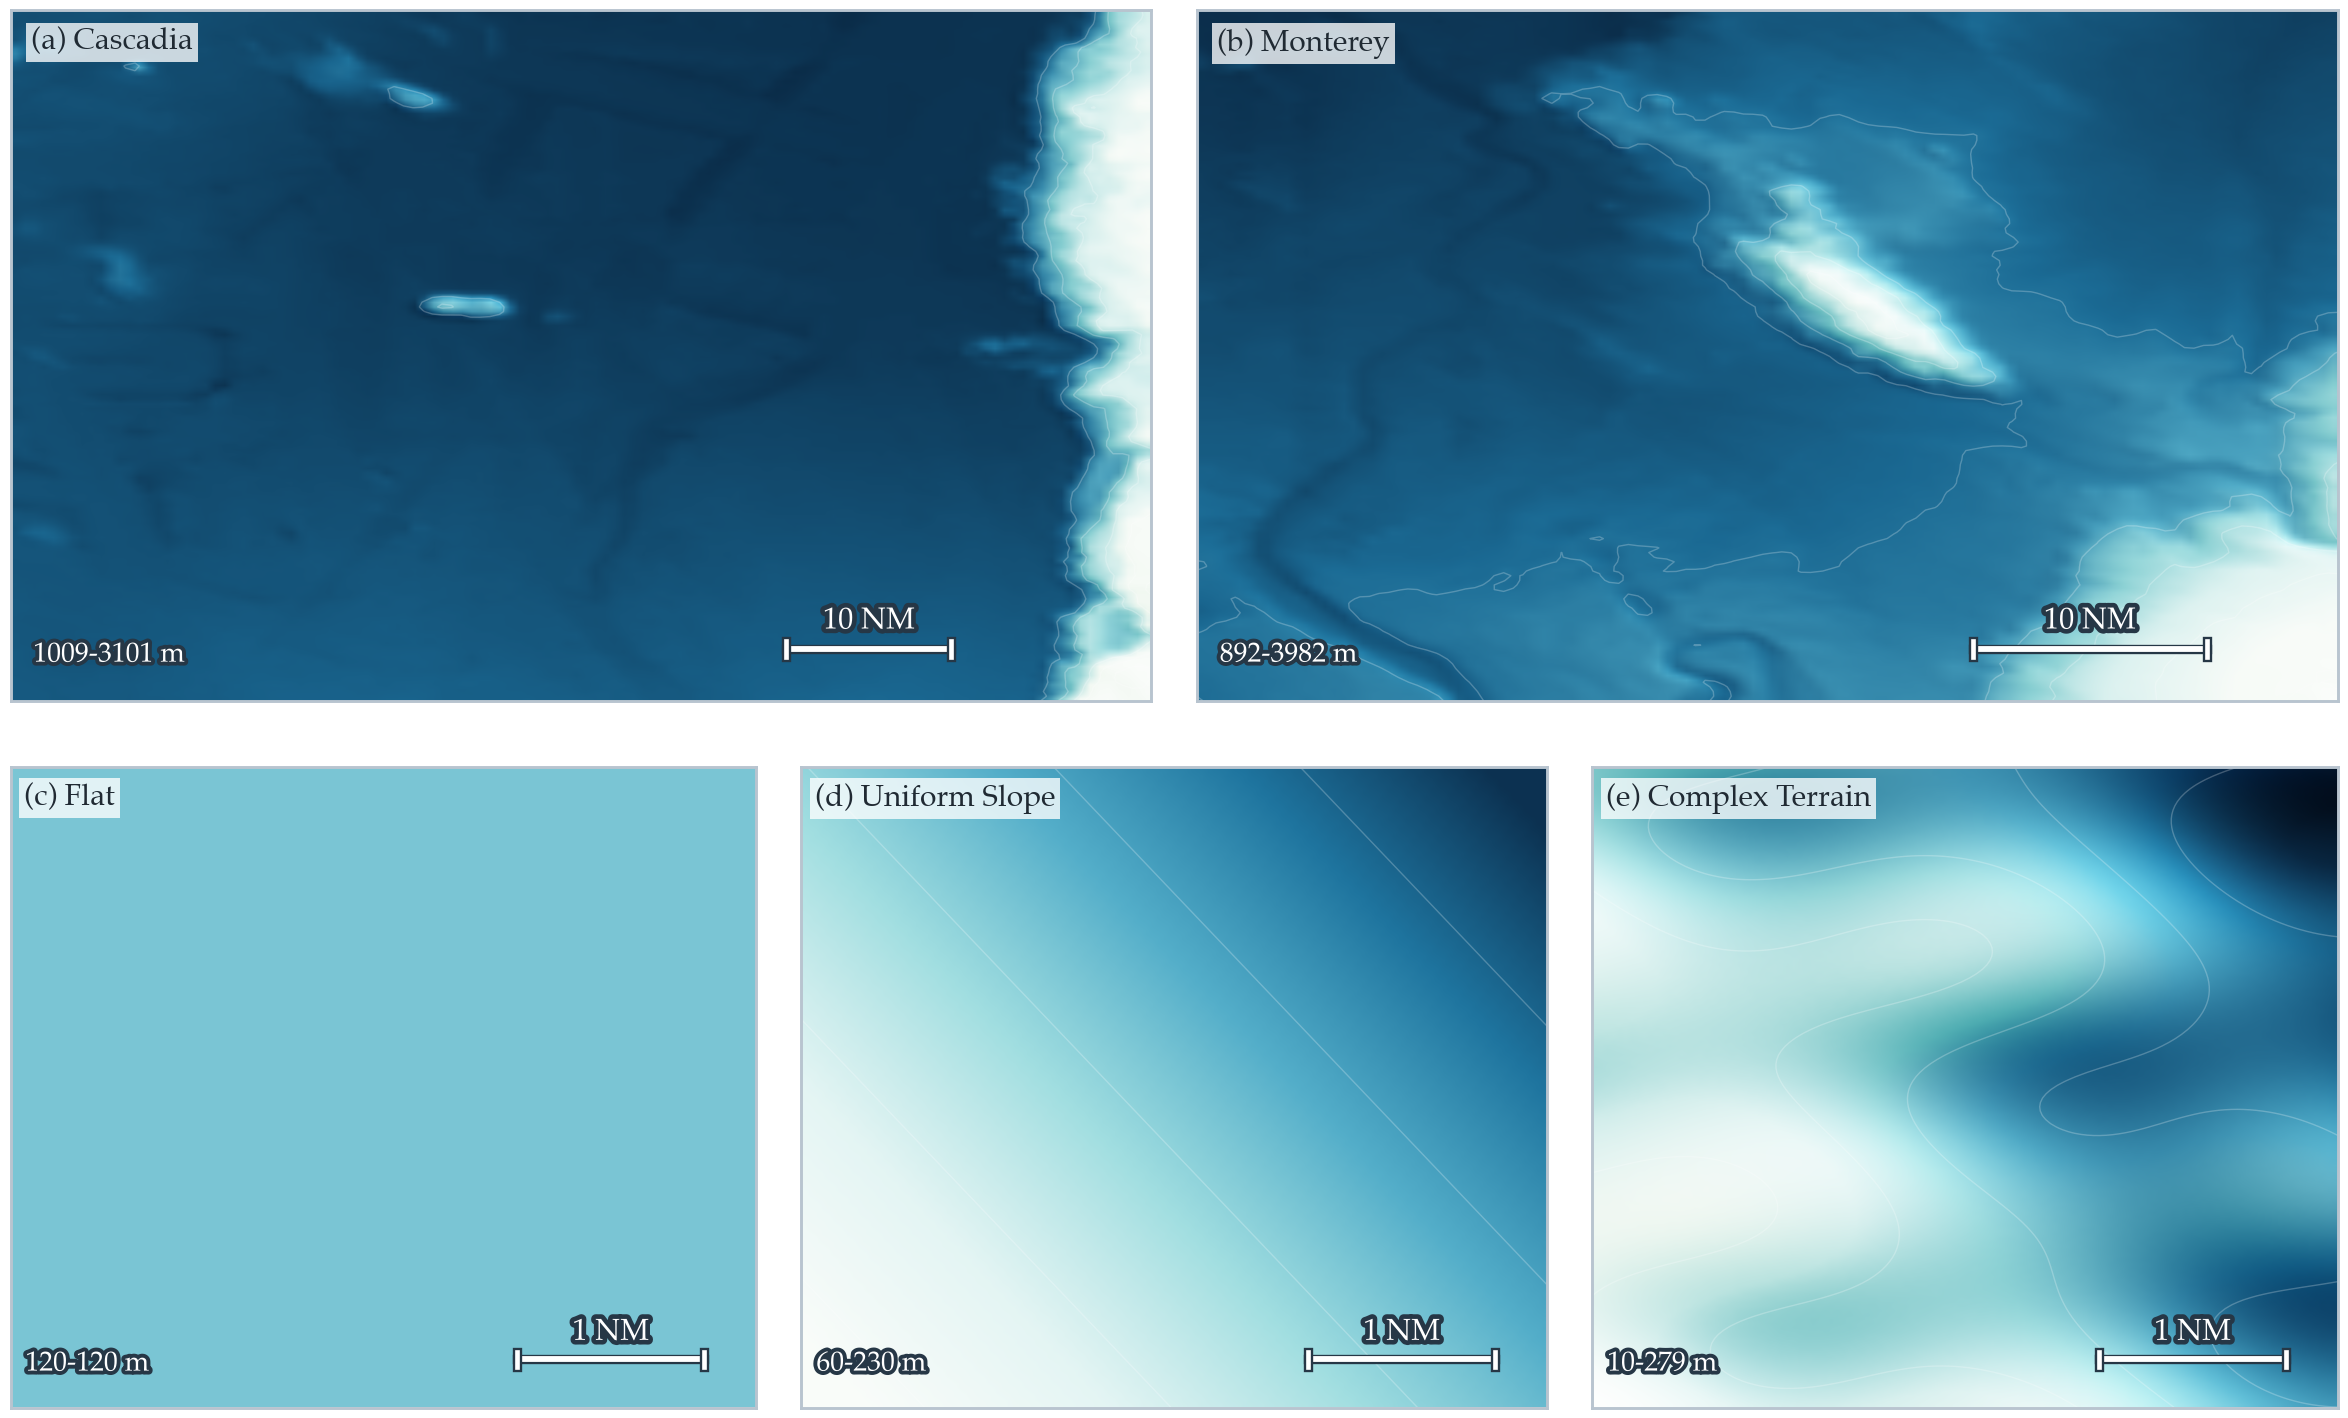
\includegraphics[width=\textwidth]{pic/journal_scene_atlas.png}
		\caption{Benchmark atlas for the five terrains used in this study. Panels (a) and (b) are public GEBCO~2025 bathymetry subsets used as the main external-data benchmark; panel (c) clarifies the evidence roles; panels (d)--(f) are synthetic stress-test terrains used to isolate flat, sloped, and complex-relief mechanisms. The map cards are rendered without axis distortion and preserve their own depth ranges because the public and synthetic scenes differ substantially in physical extent and relief.}
	\label{fig:env}
\end{figure}

\subsection{Public-scene External-Data Evidence}
Figures~\ref{fig:cascadia_routes} and~\ref{fig:monterey_routes} present the two public results as three method-specific zoom cards plus a compact summary strip. The zoom cards highlight local line-placement differences on the same terrain window, while the summary strip keeps the full-scene metrics in a single compact row. The format separates visible geometry changes from small metric cleanup without turning the figure into a full-page map. On GEBCO Cascadia Margin, the fixed-spacing baseline and the two terrain-aware planners all retain a horizontal sweep family, and the difference between Adaptive Spacing without GA and the Full Geometry-Aware Hybrid GA is small. On GEBCO Monterey Canyon, terrain-aware adaptation rotates the survey family from the baseline's $0^{\circ}$ heading to a $90^{\circ}$ heading and reduces the line count from 73 to 59. This scene is the clearest public-data example of the planner exploiting terrain geometry rather than merely tightening a fixed-spacing layout.

\begin{figure}[!htbp]
		\centering
		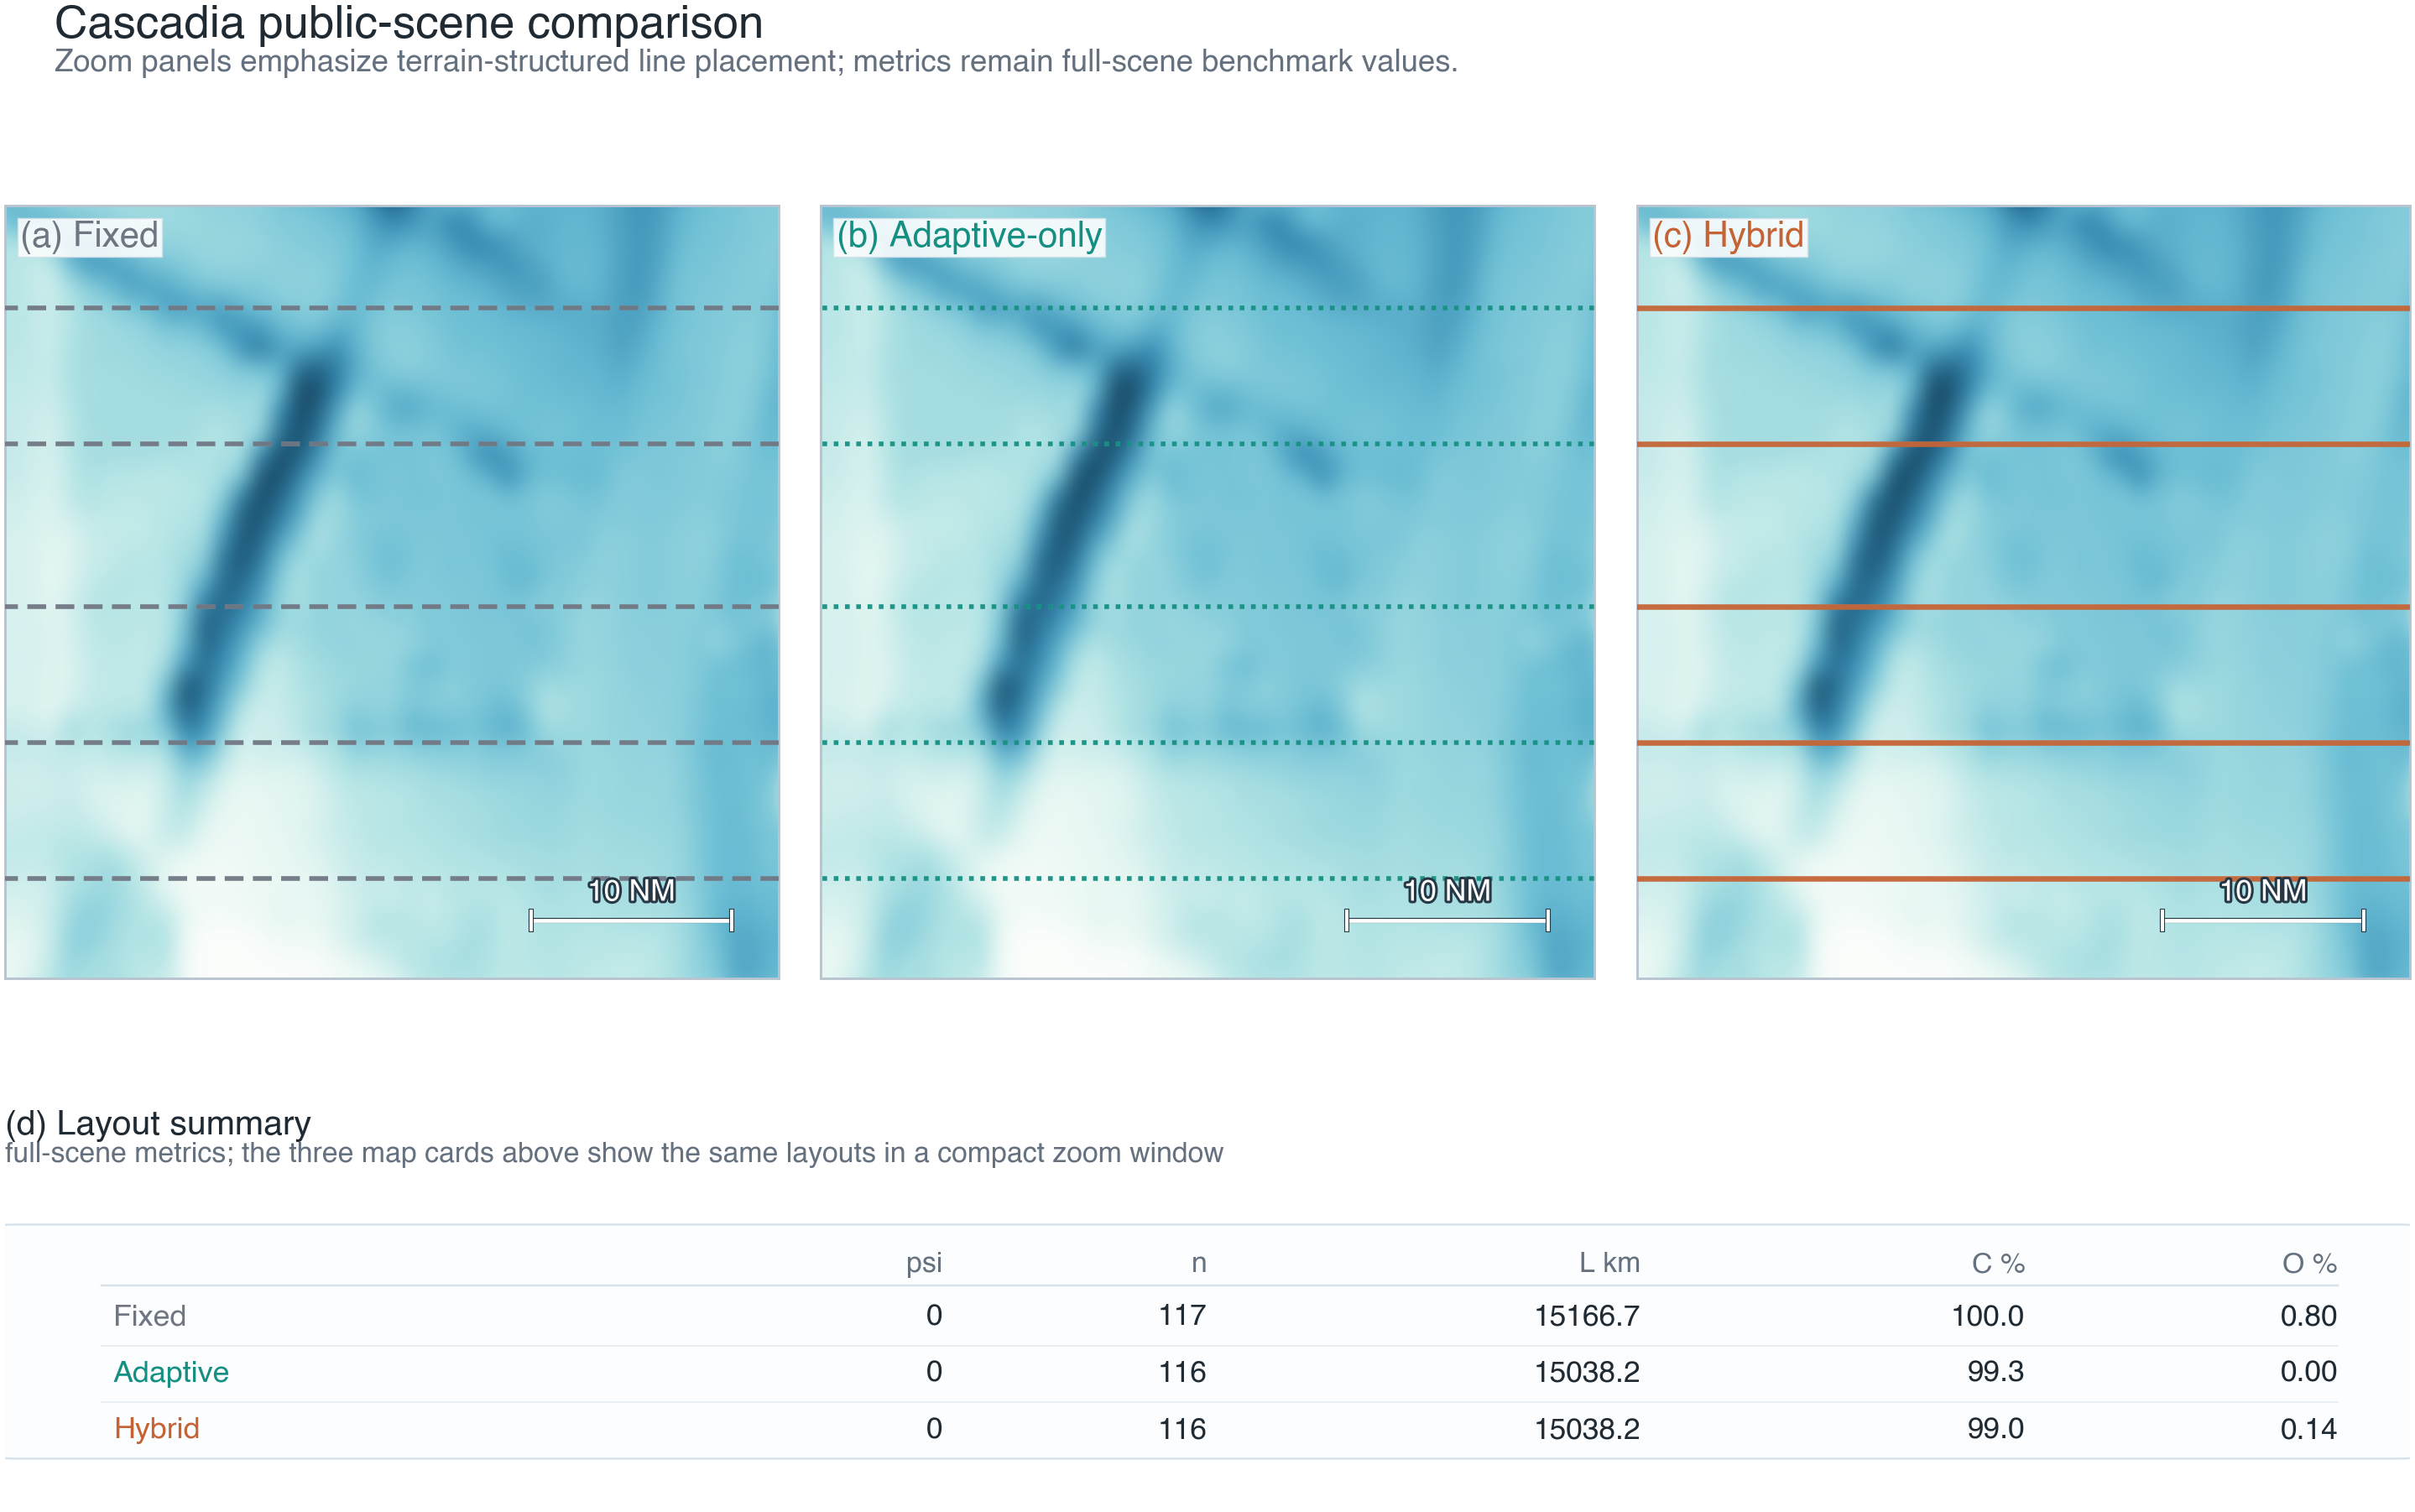
\includegraphics[width=\textwidth]{pic/journal_cascadia_routes.png}
		\caption{GEBCO Cascadia Margin public-scene comparison on the benchmark reported in this study. Panels (a)--(c) show Fixed-Spacing, Adaptive Spacing without GA, and Full Geometry-Aware Hybrid GA on the same relief-focused zoom window, so the line-placement differences are readable without a large scene-level map competing for attention. Panel (d) is a compact full-scene summary strip with the heading, line count, path length \(L\), predicted coverage \(C\), and excess-overlap violation \(O\) for each method. Only representative lines are drawn for readability, but all reported metrics use the full layouts. All three methods retain the \(0^{\circ}\) sweep family in this control scene.}
		\label{fig:cascadia_routes}
\end{figure}

\noindent Cascadia functions as the moderate-relief control case for the public benchmark. The scene confirms that geometry-aware planning does not need a dramatic line-family rotation to be useful: even when all three methods retain the same horizontal sweep structure, terrain-aware spacing still removes the baseline overlap surplus and concentrates the remaining gain into cleaner line placement rather than into a visually different traversal pattern.

\begin{figure}[!htbp]
		\centering
		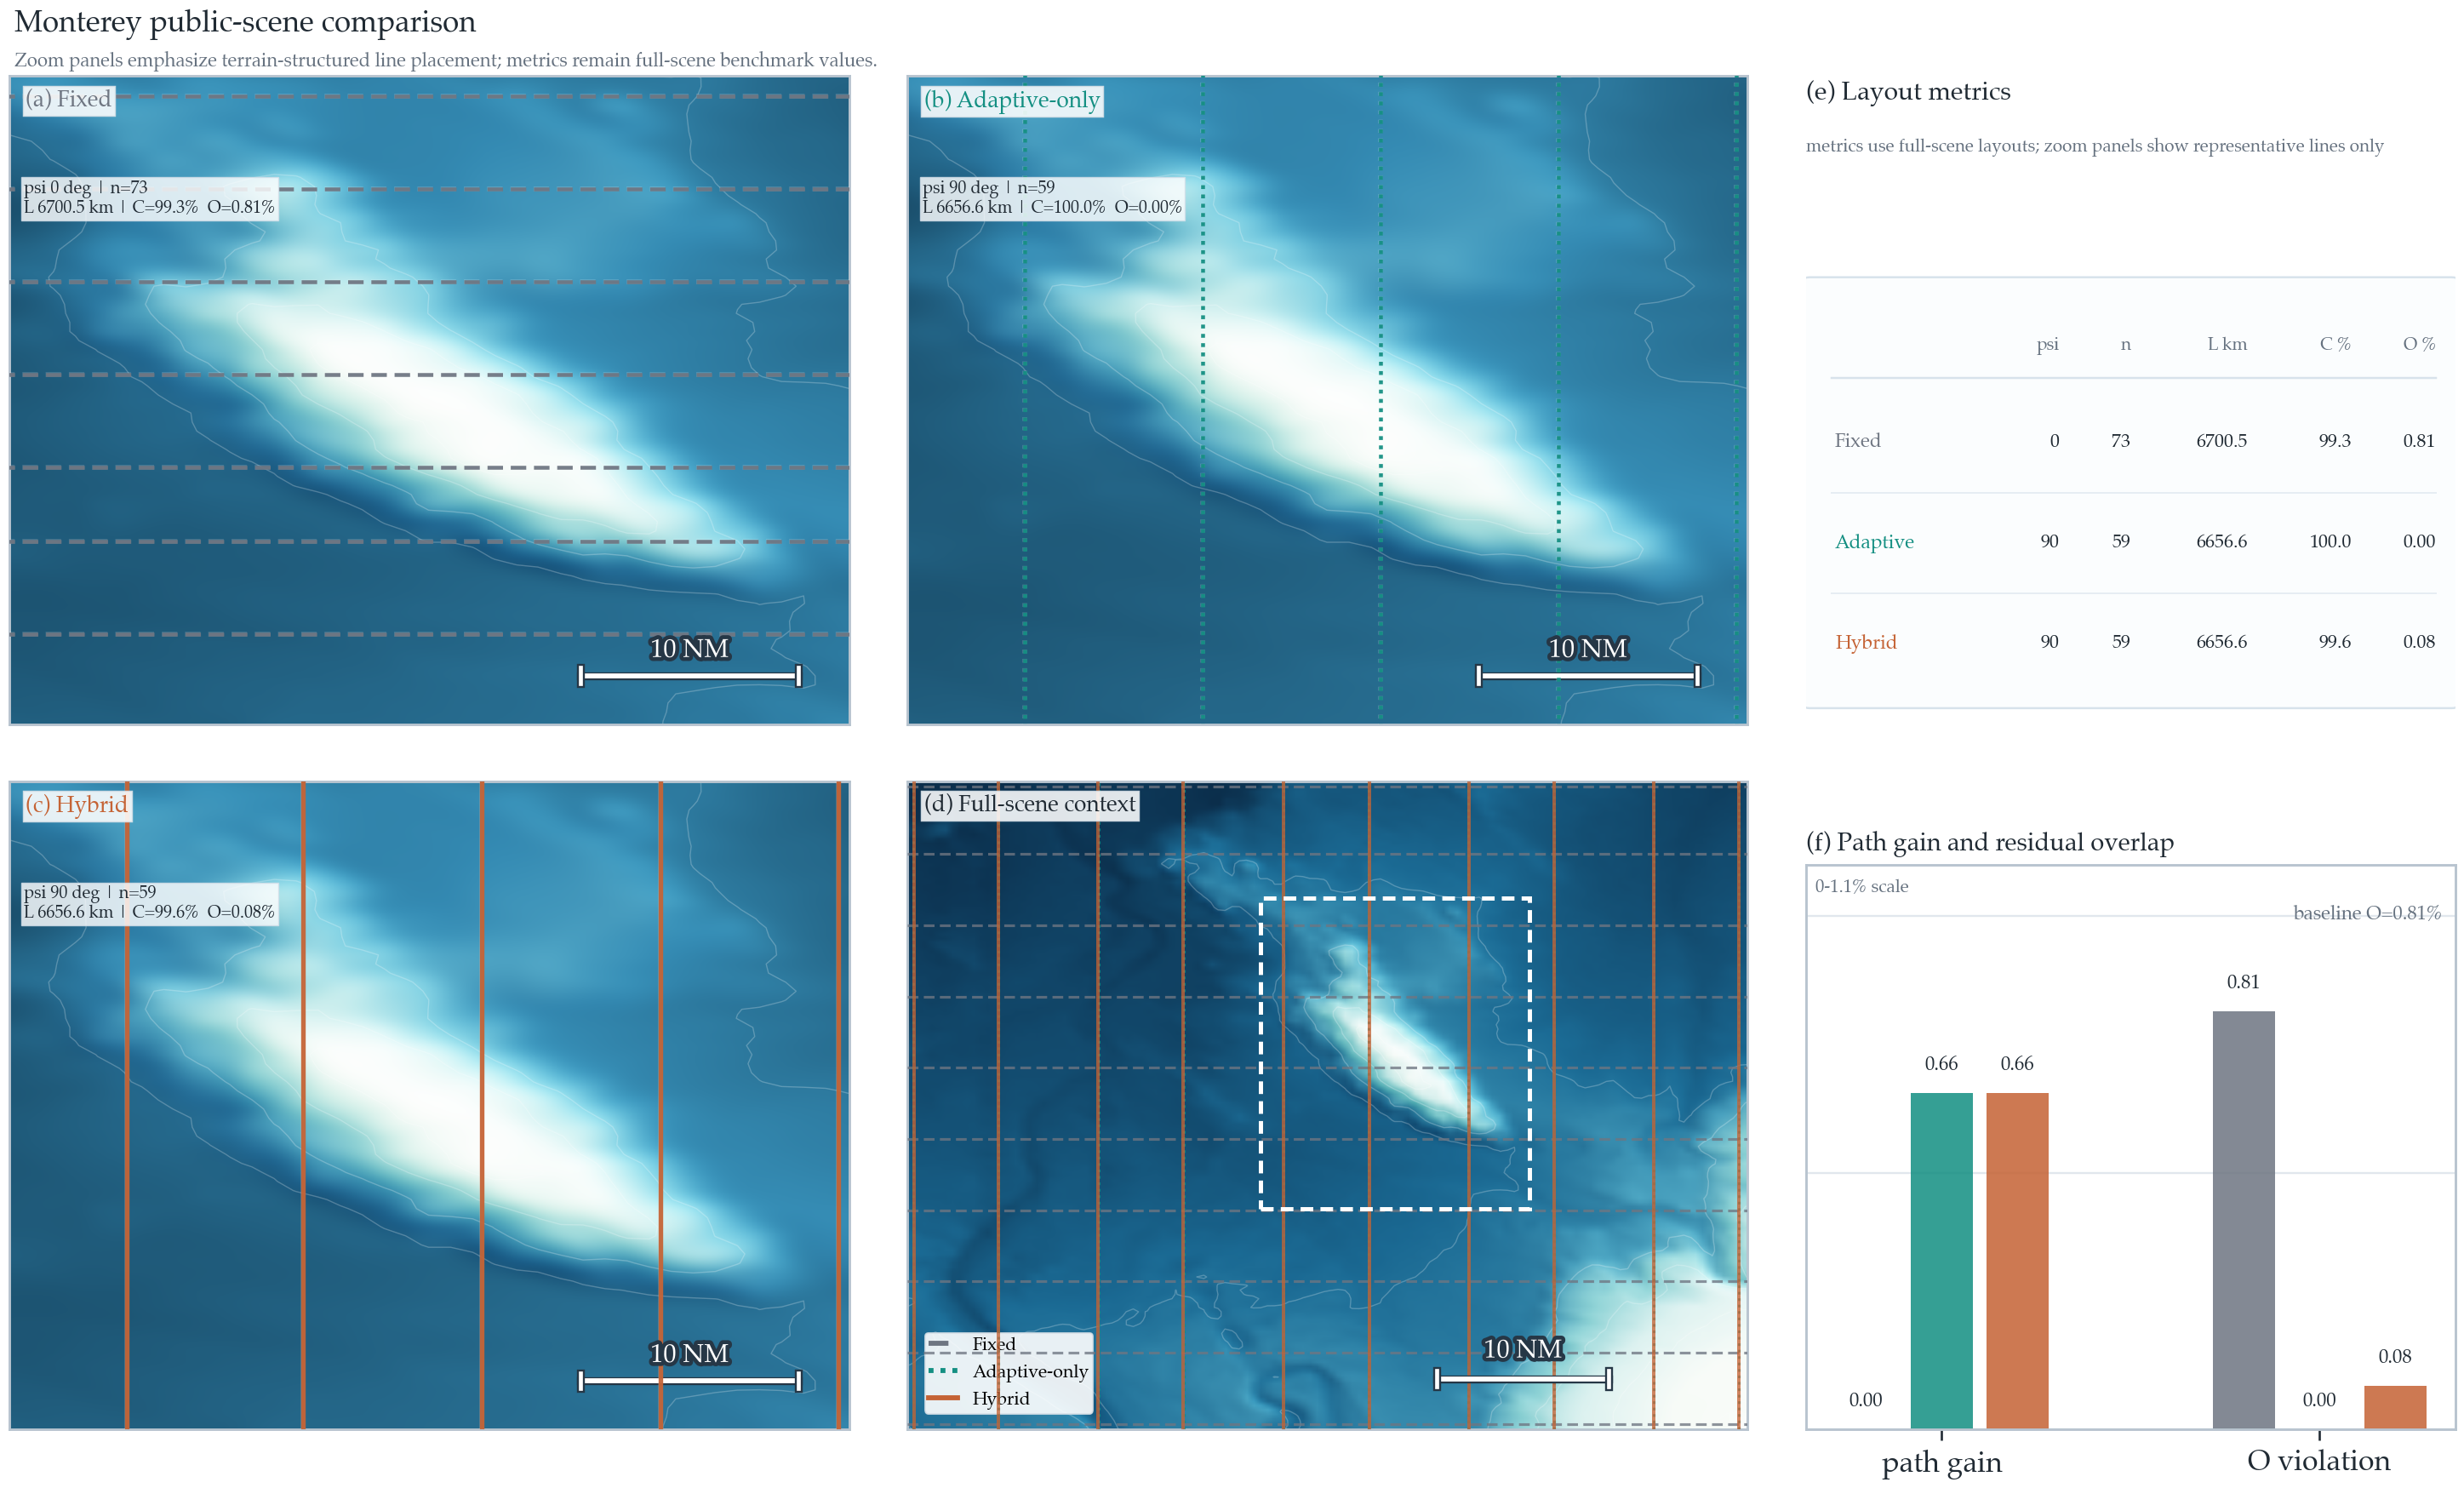
\includegraphics[width=\textwidth]{pic/journal_monterey_routes.png}
		\caption{GEBCO Monterey Canyon public-scene comparison on the benchmark reported in this study. The panel structure matches Figure~\ref{fig:cascadia_routes}: panels (a)--(c) are method-specific zooms on the same canyon window, and panel (d) is the compact full-scene summary strip with the same metric definitions. This is the strongest public-scene structural-change case: the Fixed-Spacing layout keeps the \(0^{\circ}\) family, whereas the Adaptive and Hybrid layouts rotate to \(90^{\circ}\) and reduce the line count from 73 to 59. The plotted line families are representative subsets for readability, whereas the reported metrics use the full-scene layouts.}
		\label{fig:monterey_routes}
\end{figure}

Table~\ref{tab:table2} summarizes the public-scene comparison from the reported benchmark. On the two GEBCO scenes, the reported hybrid layout achieved a 0.75 percent relative shortening of mean scene-level path length compared with the Fixed-Spacing reference, lowered mean scene-level excess-overlap violation from about 0.81 percent to 0.113 percent, and maintained mean coverage of 99.27 percent. The Simple Greedy rows show why this reference must be interpreted carefully: on Monterey, best-heading constant spacing already captures the line-count reduction and most of the route-length change, whereas terrain-aware adaptive spacing mainly improves the coverage/overlap balance. The main public result is therefore better overlap control and a cleaner fixed-line layout, rather than a large path-length reduction.

\begin{table}[!htbp]
	\centering
		\caption{Quantitative comparison on the two public GEBCO scenes from the reported benchmark. Fixed-Spacing, Simple Greedy, and Adaptive Spacing without GA are deterministic single runs. Simple Greedy is the best-heading constant-spacing baseline under the same heading scan. Full Geometry-Aware Hybrid GA reports the mean over 50 seeds. Excess overlap is the area-averaged violation above the admissible overlap ceiling of 20 percent. Lower path length, excess overlap, and planning time are better; higher predicted coverage is better.}
	\label{tab:table2}
	\scriptsize
	\renewcommand{\arraystretch}{1.15}
		\resizebox{\textwidth}{!}{%
		\begin{tabular}{@{}llccccc@{}}
		\toprule[1bp]
		\textbf{Scene} & \textbf{Method} & \textbf{Heading} & \textbf{Lines} & \textbf{Path Length (km)} & \textbf{Coverage (\%)} & \textbf{Excess Overlap (\%)} \\
		\midrule[1bp]
		\multirow{4}{*}{GEBCO Cascadia Margin} & Fixed-Spacing & \(0^{\circ}\) & 117 & 15166.71 & \textbf{100.00} & 0.80 \\
		& Simple Greedy & \(75^{\circ}\) & 111 & 15084.32 & 99.99 & 0.01 \\
		& Adaptive Spacing without GA & \(0^{\circ}\) & 116 & 15038.22 & 99.33 & \textbf{0.00} \\
		& Full Geometry-Aware Hybrid GA & \(0^{\circ}\) & 116 & \textbf{15038.15} & 98.99 & 0.14 \\
		\midrule[1bp]
		\multirow{4}{*}{GEBCO Monterey Canyon} & Fixed-Spacing & \(0^{\circ}\) & 73 & 6700.52 & 99.33 & 0.81 \\
		& Simple Greedy & \(90^{\circ}\) & 59 & \textbf{6656.37} & 99.18 & 0.30 \\
		& Adaptive Spacing without GA & \(90^{\circ}\) & 59 & 6656.62 & \textbf{100.00} & \textbf{0.00} \\
		& Full Geometry-Aware Hybrid GA & \(90^{\circ}\) & 59 & 6656.57 & 99.55 & 0.09 \\
		\bottomrule[1bp]
		\end{tabular}}
\end{table}

\noindent The two public scene cards reveal distinct mechanisms. Cascadia is mostly an overlap-control case: a best-heading constant-spacing plan already removes most of the fixed-reference overlap, while adaptive spacing gives the shortest terrain-aware layout without changing the sweep family. Monterey is the stronger structural-change case: both Simple Greedy and terrain-aware planning rotate the family to \(90^{\circ}\) and collapse the line count from 73 to 59, showing that a fair constant-spacing heading baseline captures much of the route-length effect. In both scenes, however, the gap between Adaptive Spacing without GA and the Full Hybrid GA remains very small in path length, and the deterministic adaptive layout has lower residual excess overlap on the GEBCO pair. The public-scene ablation therefore narrows the contribution claim: the public benefit is better overlap discipline and layout regularization under a fixed traversal, while GA should be read as a small local refinement and seed-repeatability layer rather than as the main overlap-control mechanism.

To make the vehicle-kinematics issue explicit without claiming field execution, Figure~\ref{fig:vehicle_aware_posteval} adds a post-planning vehicle-aware diagnostic. The diagnostic keeps the reported line families fixed, adds semicircular line-change arcs for \(R_{\min}=25\), 50, and 100~m, and converts distance into a mission-time proxy using 1.5~m/s for survey and transit distance and 0.75~m/s for turn arcs. It is deliberately a first-order execution proxy, not a Dubins controller, current-aware simulation, SLAM replay, or sea-trial validation. The GEBCO public-scene interpretation is unchanged: at \(R_{\min}=100\)~m, the hybrid layout gives only 0.85 percent and 0.78 percent mission-time proxy gains on Cascadia and Monterey, respectively. The diagnostic becomes more informative in the harder cases. On the USGS high-complexity crop, the hybrid layout retains a 23.4 percent mission-time proxy gain because it avoids the high-overlap fixed-spacing burden, and the transition-aware segmented selector correctly retains that single-heading solution rather than adding blockwise transitions for only overlap cleanup. On the synthetic complex-relief stress case, the single-heading Hybrid layout has an apparent time advantage but remains infeasible; the transition-aware segmented layout is therefore the relevant repair, giving a feasible 11.9 percent mission-time proxy gain at \(R_{\min}=100\)~m.

\begin{figure}[!htbp]
	\centering
	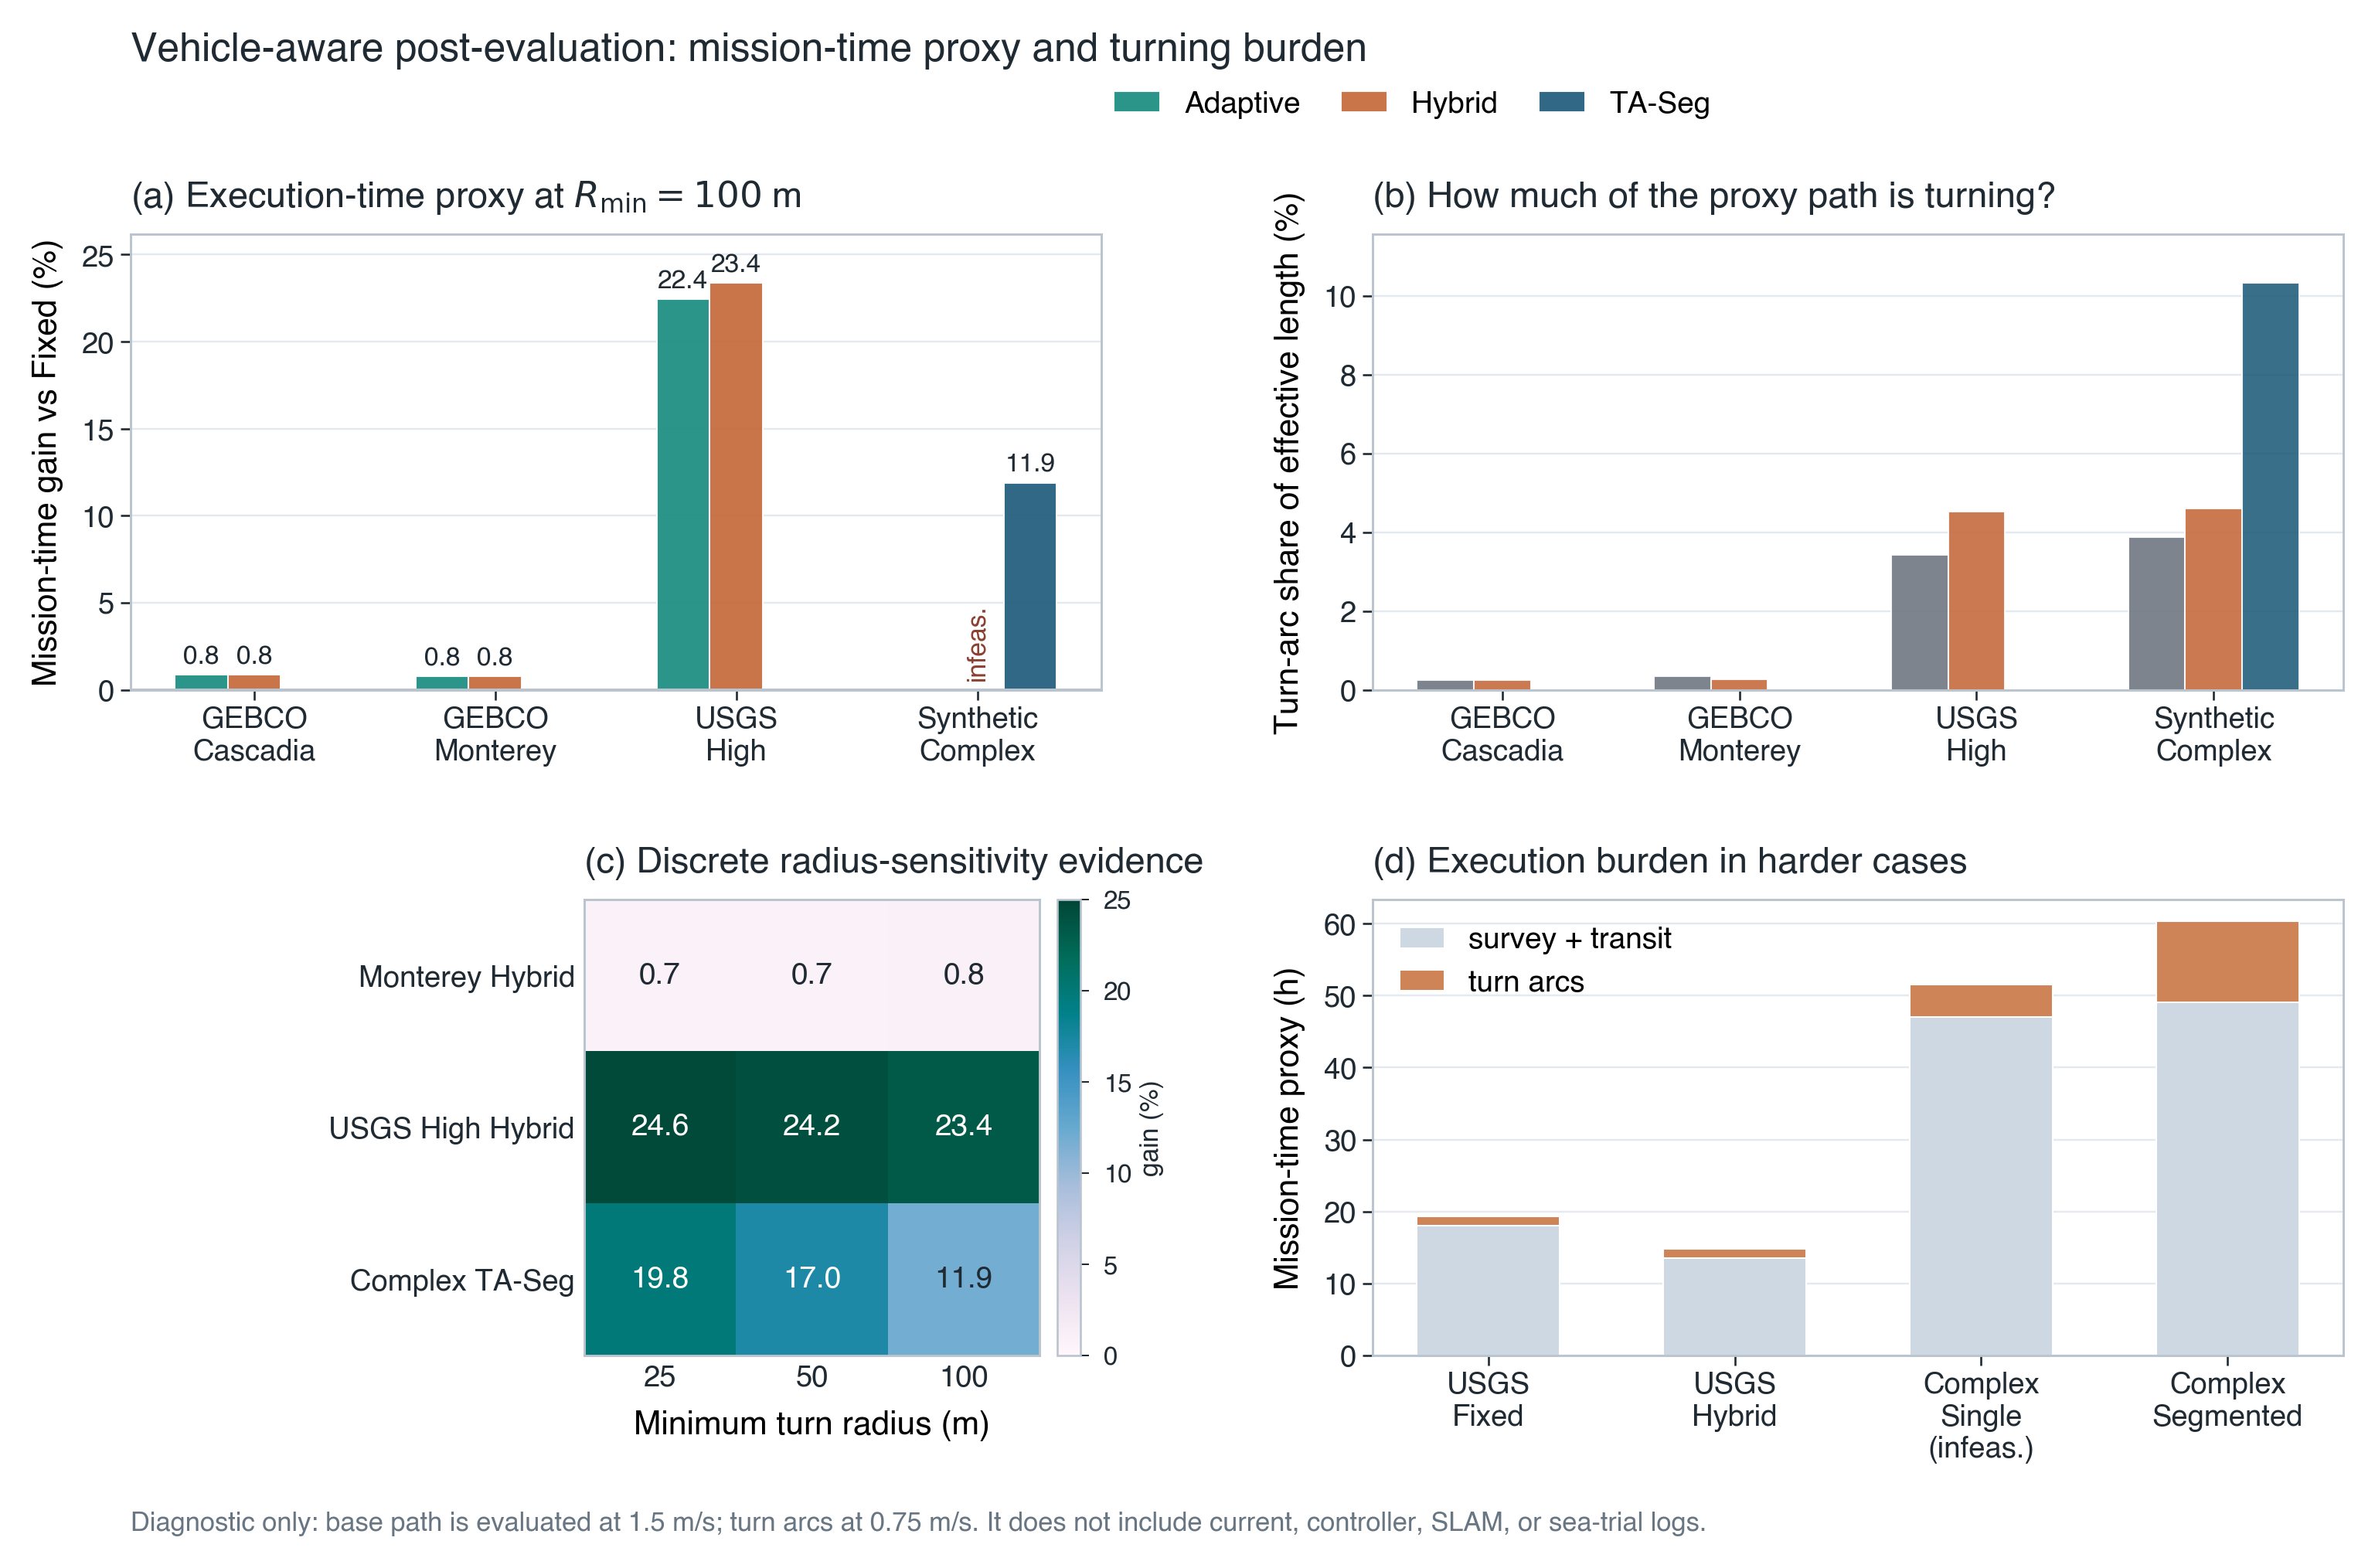
\includegraphics[width=\textwidth,height=0.44\textheight,keepaspectratio]{pic/journal_vehicle_aware_posteval.png}
	\caption{Vehicle-aware post-evaluation using a minimum-turn-radius and mission-time proxy. The diagnostic adds semicircular line-change arcs to the already reported line families, scales the turn-radius assumption from 25 to 100~m, and converts distance into time with declared survey and turn speeds. Panel (c) is shown as a discrete radius-sensitivity matrix rather than a trend curve because the three turn-radius values are declared assumptions, not sampled dynamics. Infeasible layouts are marked rather than promoted as valid gains. The figure is an execution-readiness stress check only; it does not include current, controller dynamics, SLAM feedback, or sea-trial logs.}
	\label{fig:vehicle_aware_posteval}
\end{figure}

A supplemental four-window GEBCO expansion further checks whether the two primary GEBCO windows were unusually favorable. The added Mariana Trench, Puerto Rico Trench, Mid-Atlantic Ridge, and Hawaii Ridge crops remain feasible for all tested methods under the same evaluator. Fixed-Spacing starts in the same low-overlap regime as the two primary GEBCO windows, with 0.44--0.68 percent excess overlap. Adaptive Spacing without GA removes this excess overlap and yields 0.49--0.68 percent path gain, while the 50-seed hybrid layout produces nearly the same path-gain range with residual excess overlap of 0.04--0.26 percent and feasible seed rate 1.0. This expansion does not prove geographic representativeness, but it makes the public-data story less dependent on only two hand-visible scenes: additional GEBCO windows also behave like low-overlap public-grid cases where terrain-aware spacing mainly improves overlap discipline rather than producing large route compression.

To avoid leaving the public-window evidence as only a verbal extension, Table~\ref{tab:public_window_stats} pools the two main GEBCO scenes, the four supplemental GEBCO windows, and the three USGS 30~m crops into a nine-window paired public-data audit. The table is computed from the existing CSV summaries rather than by redefining the main benchmark mean. Across the nine public windows, both Adaptive Spacing and Hybrid GA improve overlap in every window, with one-sided Wilcoxon \(p=0.00195\) and rank-biserial effect size 1.00 for overlap cleanup. Path gain is positive in 7 of 9 windows for both terrain-aware methods, with median gains of 0.681\% and one-sided Wilcoxon \(p=0.00977\). Coverage deltas are mixed, especially for Hybrid GA, which is why the manuscript continues to treat GA cleanup as gate-controlled local refinement rather than as an unconditional improvement.

The same audit is more informative when read by regime. Eight public windows start in a low-overlap regime with Fixed-Spacing excess overlap below \(3\%\); in that group, Adaptive Spacing has median path gain 0.668\% and median overlap cleanup 0.740 percentage points, while Hybrid GA has median path gain 0.669\% and median overlap cleanup 0.635 percentage points. The only overlap-stressed public window is the USGS high-complexity crop, where Fixed-Spacing begins at 29.96\% excess overlap and the gains are much larger: 24.02\% path gain with 27.72 percentage-point overlap cleanup for Adaptive Spacing and 25.04\% path gain with 28.23 percentage-point cleanup for Hybrid GA. The study therefore does not claim a uniform percentage gain across bathymetric settings; it claims a regime-dependent effect in which terrain-aware spacing mostly regularizes low-overlap public priors and becomes a stronger intervention when the prior reveals a high-overlap spacing burden.

\begin{table}[!htbp]
	\centering
	\caption{Paired public-window statistics across nine public bathymetry windows. Values are computed from the two primary GEBCO scenes, four supplemental GEBCO windows, and three USGS 30~m crops. \(G_L\) is path gain relative to Fixed-Spacing, \(\Delta O\) is overlap cleanup, and \(\Delta C\) is coverage change. CI denotes a 95\% bootstrap interval for the window-level mean; \(p\) is a one-sided Wilcoxon signed-rank test for a positive paired delta.}
	\label{tab:public_window_stats}
	\scriptsize
	\renewcommand{\arraystretch}{1.12}
	\setlength{\tabcolsep}{4.0pt}
	\begin{tabular}{@{}>{\raggedright\arraybackslash}p{0.34\linewidth}>{\centering\arraybackslash}p{0.28\linewidth}>{\centering\arraybackslash}p{0.28\linewidth}@{}}
		\toprule[1bp]
		\textbf{Statistic} & \textbf{Adaptive Spacing} & \textbf{Hybrid GA} \\
		\midrule[1bp]
		Feasible public windows & 9/9 & 9/9 \\
		\(G_L\) median (\%) & 0.681 & 0.681 \\
		\(G_L\) mean [95\% CI] (\%) & 3.041 [0.198, 8.378] & 3.213 [0.315, 8.734] \\
		Positive \(G_L\) windows / \(p_G\) / \(r_{rb,G}\) & 7/9 / 0.00977 / 0.867 & 7/9 / 0.00977 / 0.867 \\
		\(\Delta O\) median (pp) & 0.799 & 0.663 \\
		\(\Delta O\) mean [95\% CI] (pp) & 3.895 [0.719, 9.920] & 3.869 [0.595, 10.045] \\
		Positive \(\Delta O\) windows / \(p_O\) / \(r_{rb,O}\) & 9/9 / 0.00195 / 1.000 & 9/9 / 0.00195 / 1.000 \\
		\(\Delta C\) median (pp) & 0.000 & -0.933 \\
		Positive \(\Delta C\) windows / \(p_C\) / \(r_{rb,C}\) & 2/9 / 0.59375 / -0.048 & 2/9 / 0.94922 / -0.600 \\
		\bottomrule[1bp]
	\end{tabular}
\end{table}

\subsection{Cross-scene Mechanism and Failure Boundary}
The synthetic stress tests clarify both why the public gains are limited and where the present method breaks. On Flat Seafloor, the reported hybrid layout achieved a 3.56 percent relative route shortening compared with Fixed-Spacing and eliminated mean excess-overlap violation while remaining feasible. This flat-case gain should not be interpreted as a terrain-understanding effect. Because the baseline fixes the reference heading and uses a discrete line-count and boundary-clipping construction, even a planar test can expose line-count quantization and edge effects; the flat scene is therefore a baseline sanity check and a reminder that not every route gain comes from relief-dependent footprint adaptation. On Uniform Slope, where cross-track geometry is no longer flat, the path gain increased to 7.69 percent, with near-saturated predicted coverage (99.999 percent) and only 0.044 percent excess overlap. On the hardest Complex Terrain scene, the route shortened from 342.38~km to 254.13~km and excess overlap fell from 28.50 percent to 7.18 percent, but coverage remained at 96.82 percent and the feasibility flag stayed 0.0 across seeds. Adaptive Spacing without GA was almost identical on that scene, so the results reveal a genuine failure case rather than a solved benchmark. Figure~\ref{fig:failure_mode_complex} visualizes the failure rather than only reporting the aggregate metric: terrain-aware layouts move the zero-coverage cells away from the broad Fixed-Spacing gap pattern and lower the large overlap field, but localized uncovered patches remain in the complex-relief scene. The most likely interpretation is that terrain-aware spacing is necessary but not sufficient once relief becomes too heterogeneous for a single-heading parallel-line family to represent the survey efficiently.

	\begin{figure}[!htbp]
		\centering
		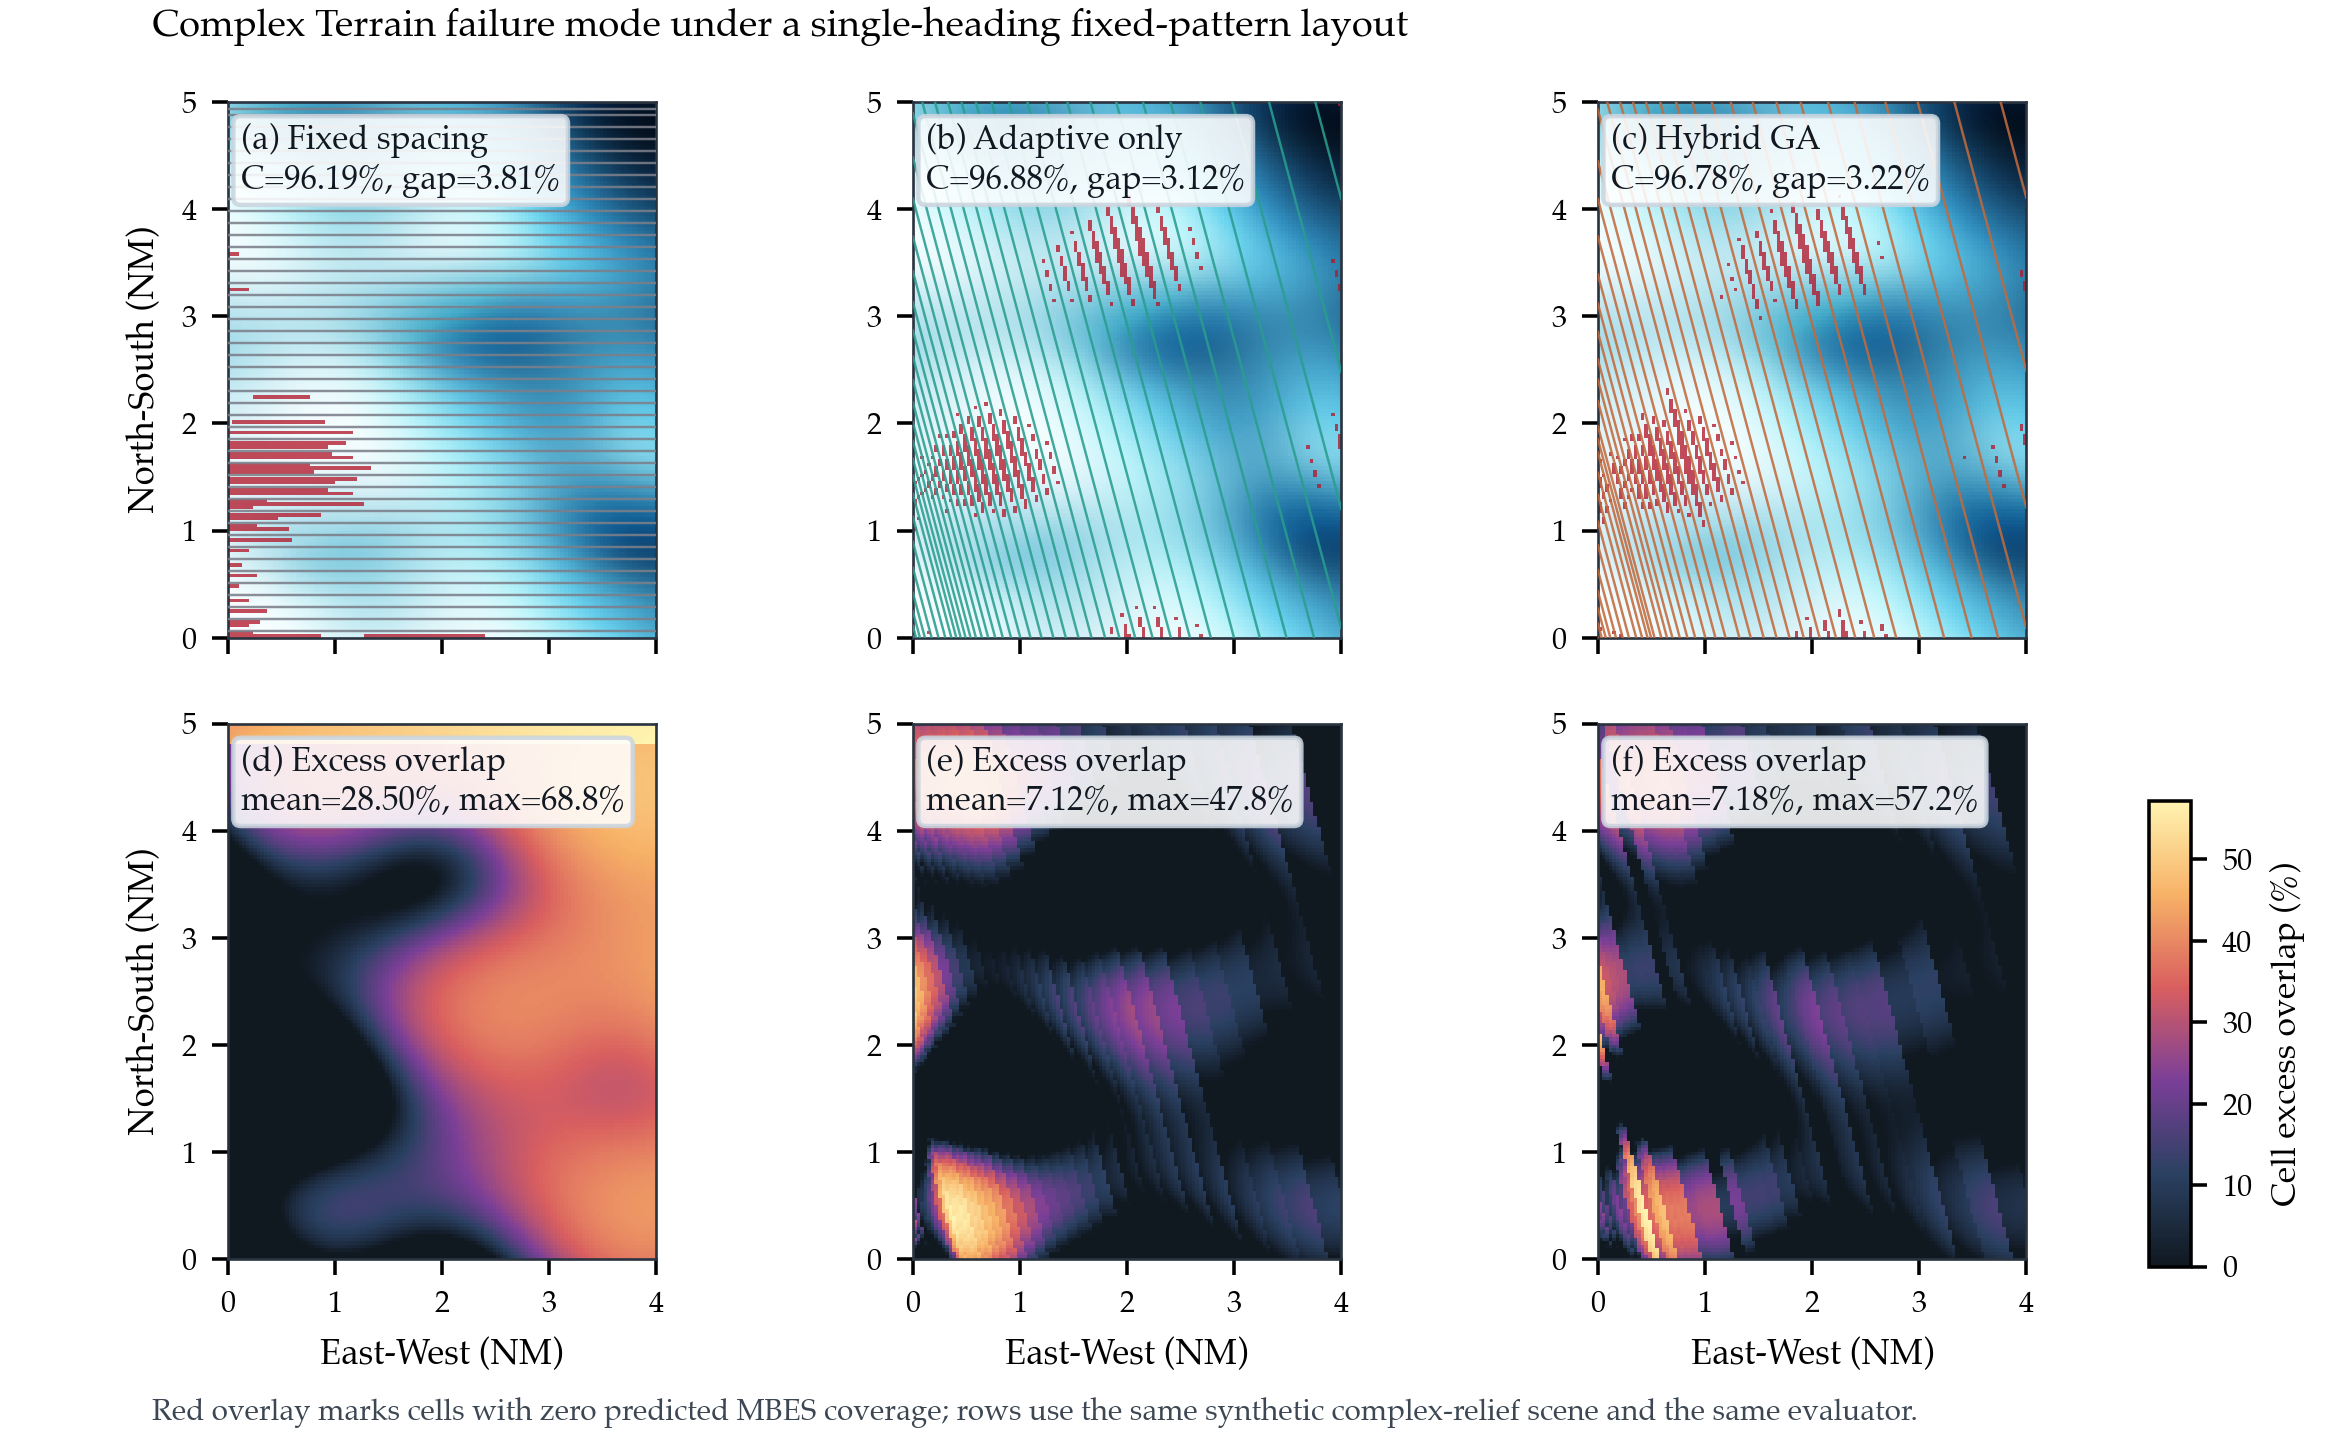
\includegraphics[width=\textwidth]{pic/journal_failure_mode_complex.png}
		\caption{Failure-mode visualization for the synthetic Complex Terrain stress test. Panels (a)--(c) overlay zero-predicted-coverage cells in red on the terrain and planned line family for Fixed-Spacing, Adaptive Spacing without GA, and a representative Hybrid GA run. Panels (d)--(f) show the corresponding cellwise excess-overlap fields; the single gradient colorbar is shared only by these bottom-row panels because the top row uses a binary red gap overlay rather than a continuous field. The figure is recomputed from \texttt{run\_5/complex\_terrain\_failure\_mode\_summary.csv} and the same sensor--terrain evaluator as the main benchmark. The result is a numerical boundary-of-validity diagnostic: adaptive spacing lowers the overlap field but does not remove all predicted gaps under the present single-heading fixed-pattern assumption.}
		\label{fig:failure_mode_complex}
	\end{figure}

The failure visualization also points to a constrained extension: the planner needs more than one line-family heading when relief changes substantially across the same survey box. We therefore added a separate transition-aware segmented-heading diagnostic that splits the survey rectangle into a small number of cross-track blocks, keeps multiple candidate line families per block, and scores candidate combinations with boundary-transit and heading-change terms. The reported length includes conservative boundary transits and a minimum-turn-radius heading-change term with \(R_{\min}=100\)~m. A segmented candidate is first accepted only if it satisfies the global 97 percent coverage and 3 percent excess-overlap gates and does not reduce coverage relative to the single-heading Hybrid GA unless it converts an infeasible single-heading layout into a feasible one. After this gate, we report both a coverage-preserving selector based on \(L+3O_{\mathrm{ex}}\) and a stricter transition-aware selector that ranks the surviving single-heading and blockwise candidates by a declared mission-time proxy at \(R_{\min}=100\)~m, including semicircular line-change arcs and slower turn speed. We report this as a blockwise layout extension rather than as part of the main single-heading benchmark.

The 30-seed run changes the earlier interpretation in a concrete way. On Complex Terrain, single-heading Hybrid GA remained infeasible (96.83 percent coverage and 7.17 percent excess overlap), so the transition-aware selector was not allowed to retain the faster but infeasible single-heading layout; it selected the four-segment repair in all 30 seeds, restoring feasibility at 97.18 percent coverage and 1.39 percent excess overlap. On GEBCO Monterey Canyon, the transition-aware selector accepted a segmented layout in 14 of 30 seeds and otherwise retained the single-heading layout, yielding 99.74 percent mean coverage, 0.049 percent mean excess overlap, and a 6.11 percent path gain relative to Fixed-Spacing. On Mariana Trench and Puerto Rico Trench, it fell back to the single-heading layout because segmented candidates shortened the route only by losing coverage. On the USGS high-complexity crop, the coverage-preserving selector would accept two-segment layouts in 8 of 30 seeds and reduce residual overlap, but the transition-aware selector rejected those blockwise plans because their added transition burden raised the mission-time proxy; it therefore retained the single-heading Hybrid GA with 98.42 percent coverage, 1.75 percent excess overlap, and a 23.37 percent mission-time proxy gain relative to Fixed-Spacing. This rejection prevents segmentation from being promoted when overlap cleanup is not worth the declared execution burden.

\begin{figure}[!htbp]
	\centering
	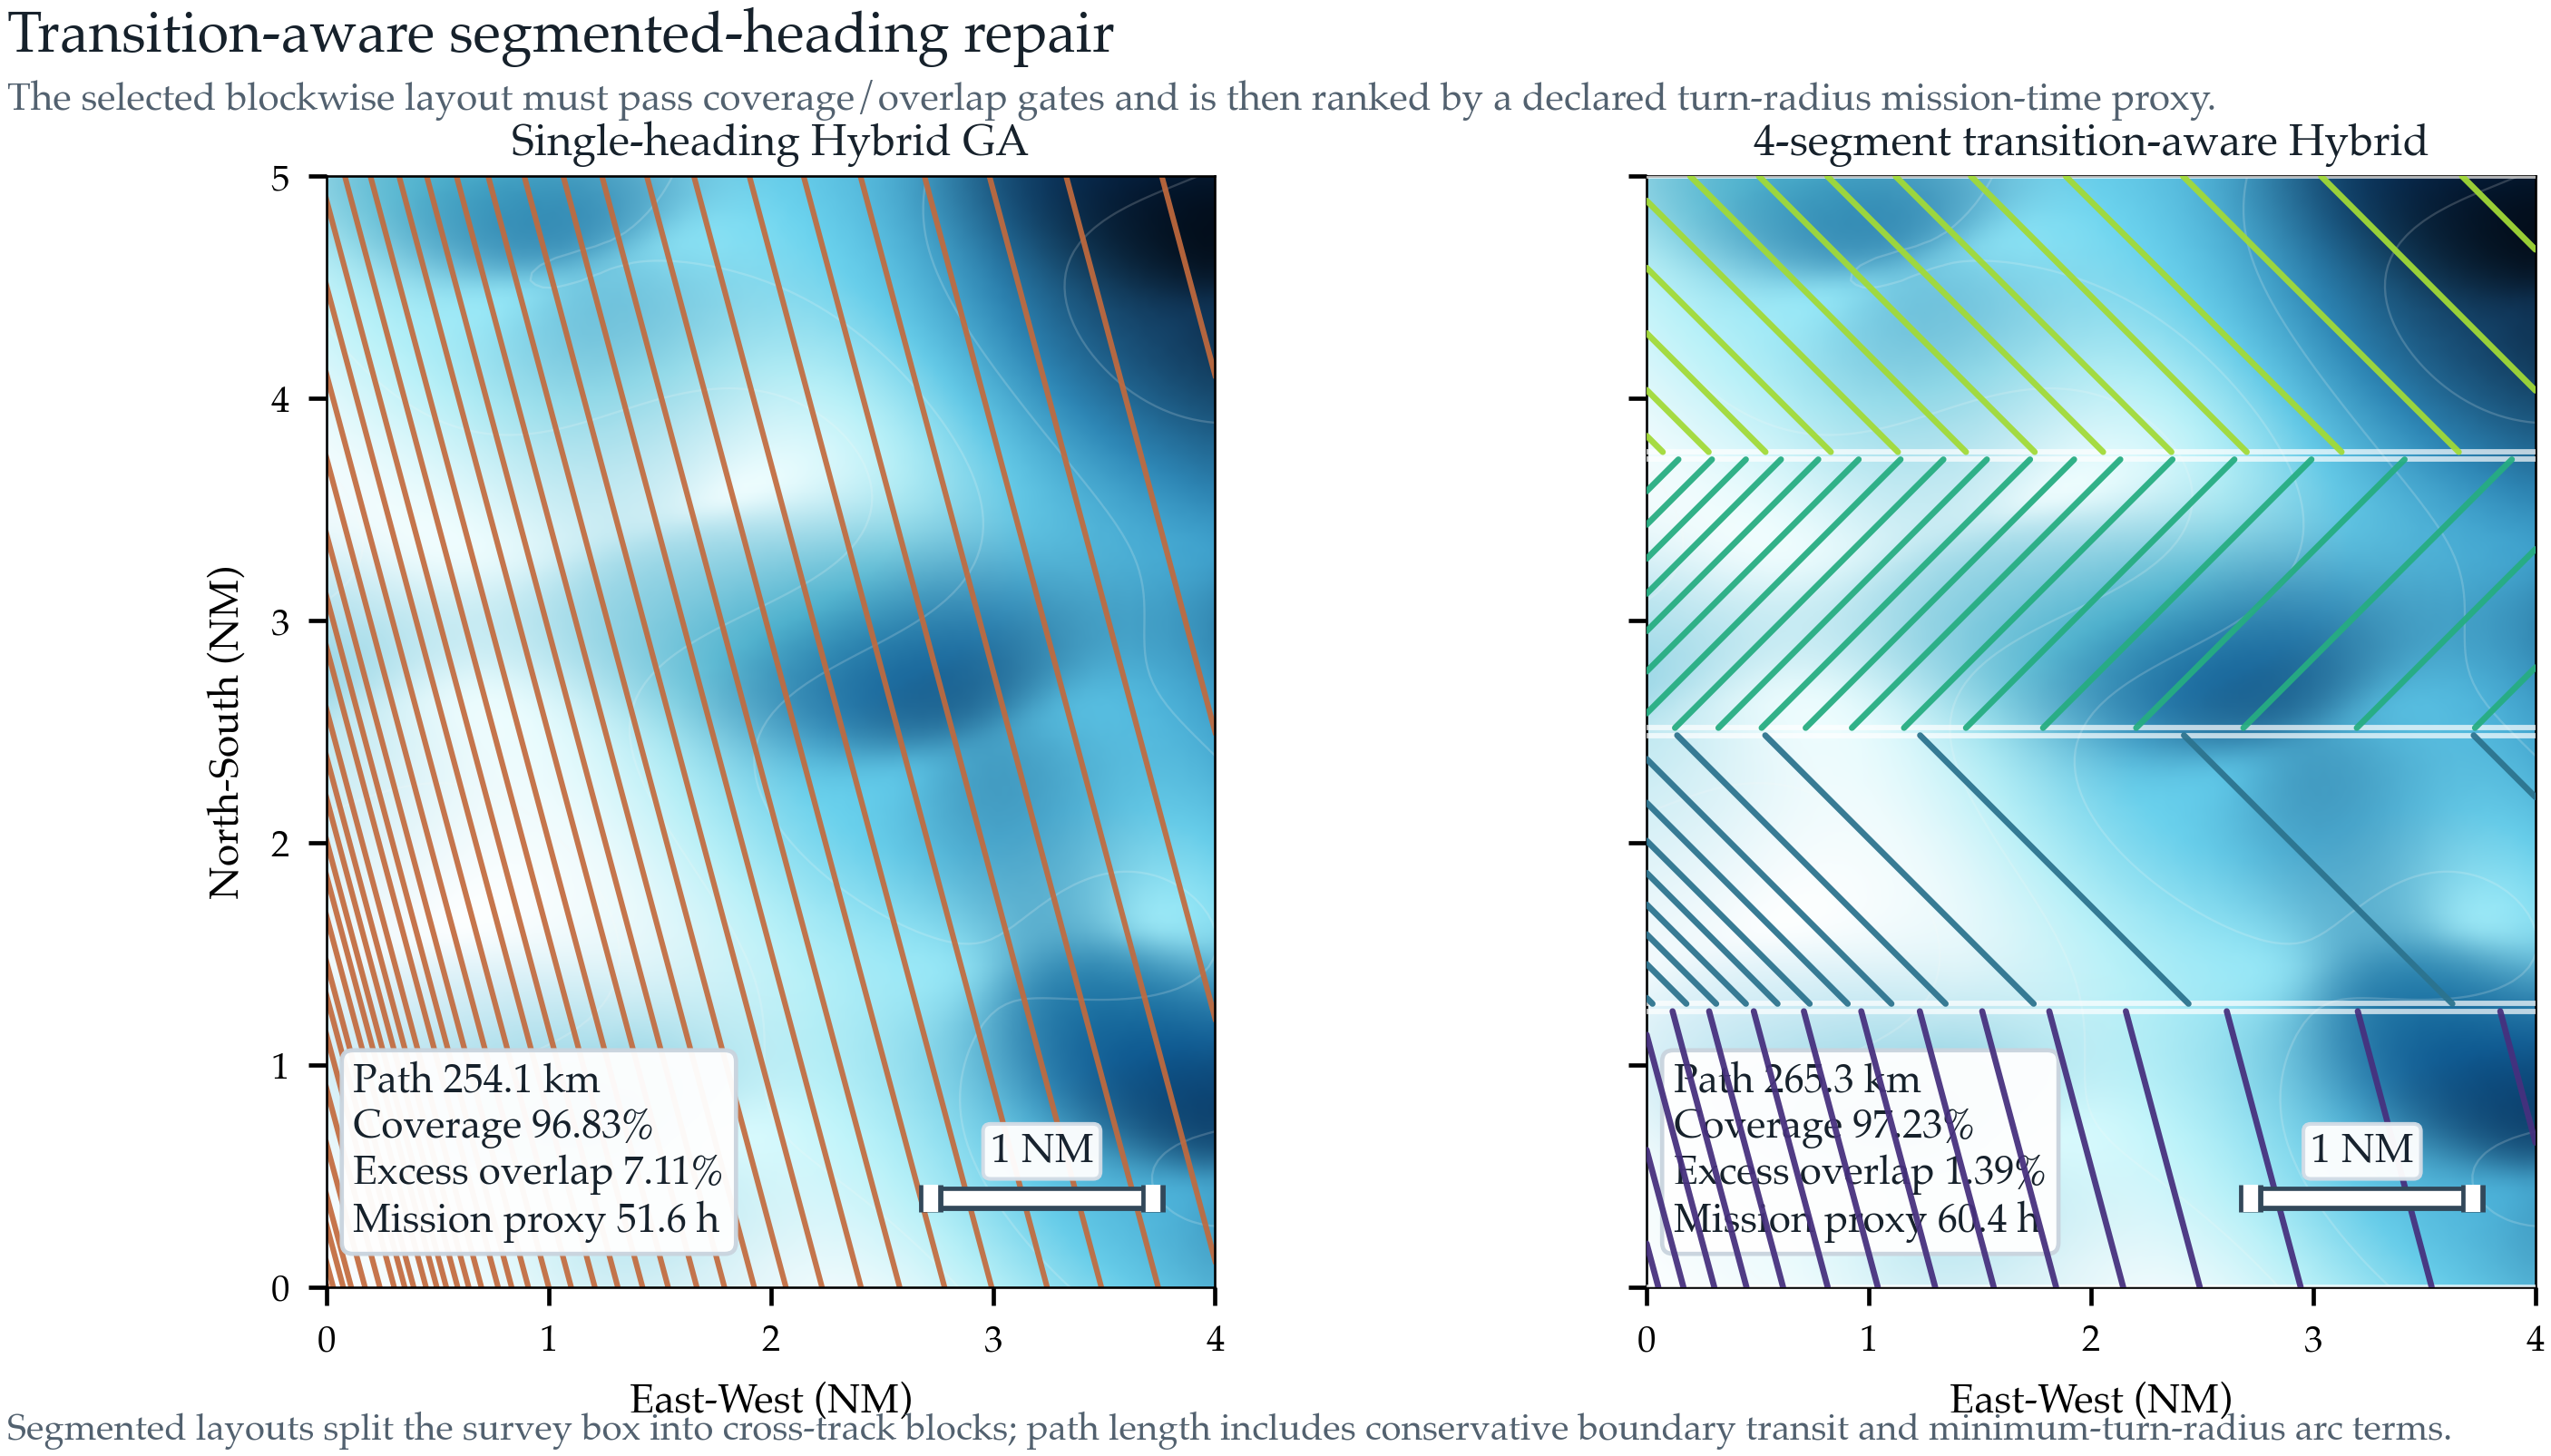
\includegraphics[width=0.96\textwidth,height=0.30\textheight,keepaspectratio]{pic/journal_segmented_heading_complex_repair.png}
	\caption{Transition-aware segmented-heading repair diagnostic for the synthetic Complex Terrain failure case. The left panel shows a representative single-heading Hybrid GA layout, which is faster under the declared mission-time proxy but remains infeasible because predicted coverage stays below the 97 percent threshold and excess overlap remains above the reported acceptance margin. The right panel shows the accepted four-segment Hybrid GA extension, where each block selects its own heading and spacing margin while the reported path length and selector include conservative inter-block transits, minimum-turn-radius heading-change terms, and line-change turn arcs. This figure is a numerical blockwise-layout diagnostic, not a sea-trial or vehicle-dynamics validation.}
	\label{fig:segmented_heading_repair}
\end{figure}

\begin{table}[!b]
	\centering
	\caption{Transition-aware segmented-heading selector diagnostic across the five complex-relief test scenes. TA-Seg denotes the final selector after the coverage/overlap gate and the declared \(R_{\min}=100\)~m mission-time proxy. Segment-selected seeds count how often a blockwise layout is selected rather than the single-heading Hybrid GA. \(C\) is predicted coverage and \(O_{\mathrm{ex}}\) is mean excess-overlap violation.}
	\label{tab:segmented_selector}
	\scriptsize
	\renewcommand{\arraystretch}{1.10}
	\resizebox{\textwidth}{!}{%
	\begin{tabular}{@{}lrrrrrr@{}}
		\toprule[1bp]
		\textbf{Scene} & \textbf{Single \(C\) (\%)} & \textbf{Single \(O_{\mathrm{ex}}\) (\%)} & \textbf{TA segment-selected seeds} & \textbf{TA-Seg \(C\) (\%)} & \textbf{TA-Seg \(O_{\mathrm{ex}}\) (\%)} & \textbf{TA-Seg path gain vs Fixed (\%)} \\
		\midrule[1bp]
		Complex Terrain & 96.83 & 7.172 & 30/30 & 97.18 & 1.392 & 22.50 \\
		GEBCO Monterey Canyon & 99.56 & 0.082 & 14/30 & 99.74 & 0.049 & 6.11 \\
		GEBCO Mariana Trench & 99.02 & 0.126 & 0/30 & 99.02 & 0.126 & 0.68 \\
		GEBCO Puerto Rico Trench & 98.08 & 0.274 & 0/30 & 98.08 & 0.274 & 0.49 \\
		USGS Cascadia 30 m High & 98.42 & 1.752 & 0/30 & 98.42 & 1.752 & 25.04 \\
		\bottomrule[1bp]
	\end{tabular}}
\end{table}

\begin{figure}[!htbp]
	\centering
	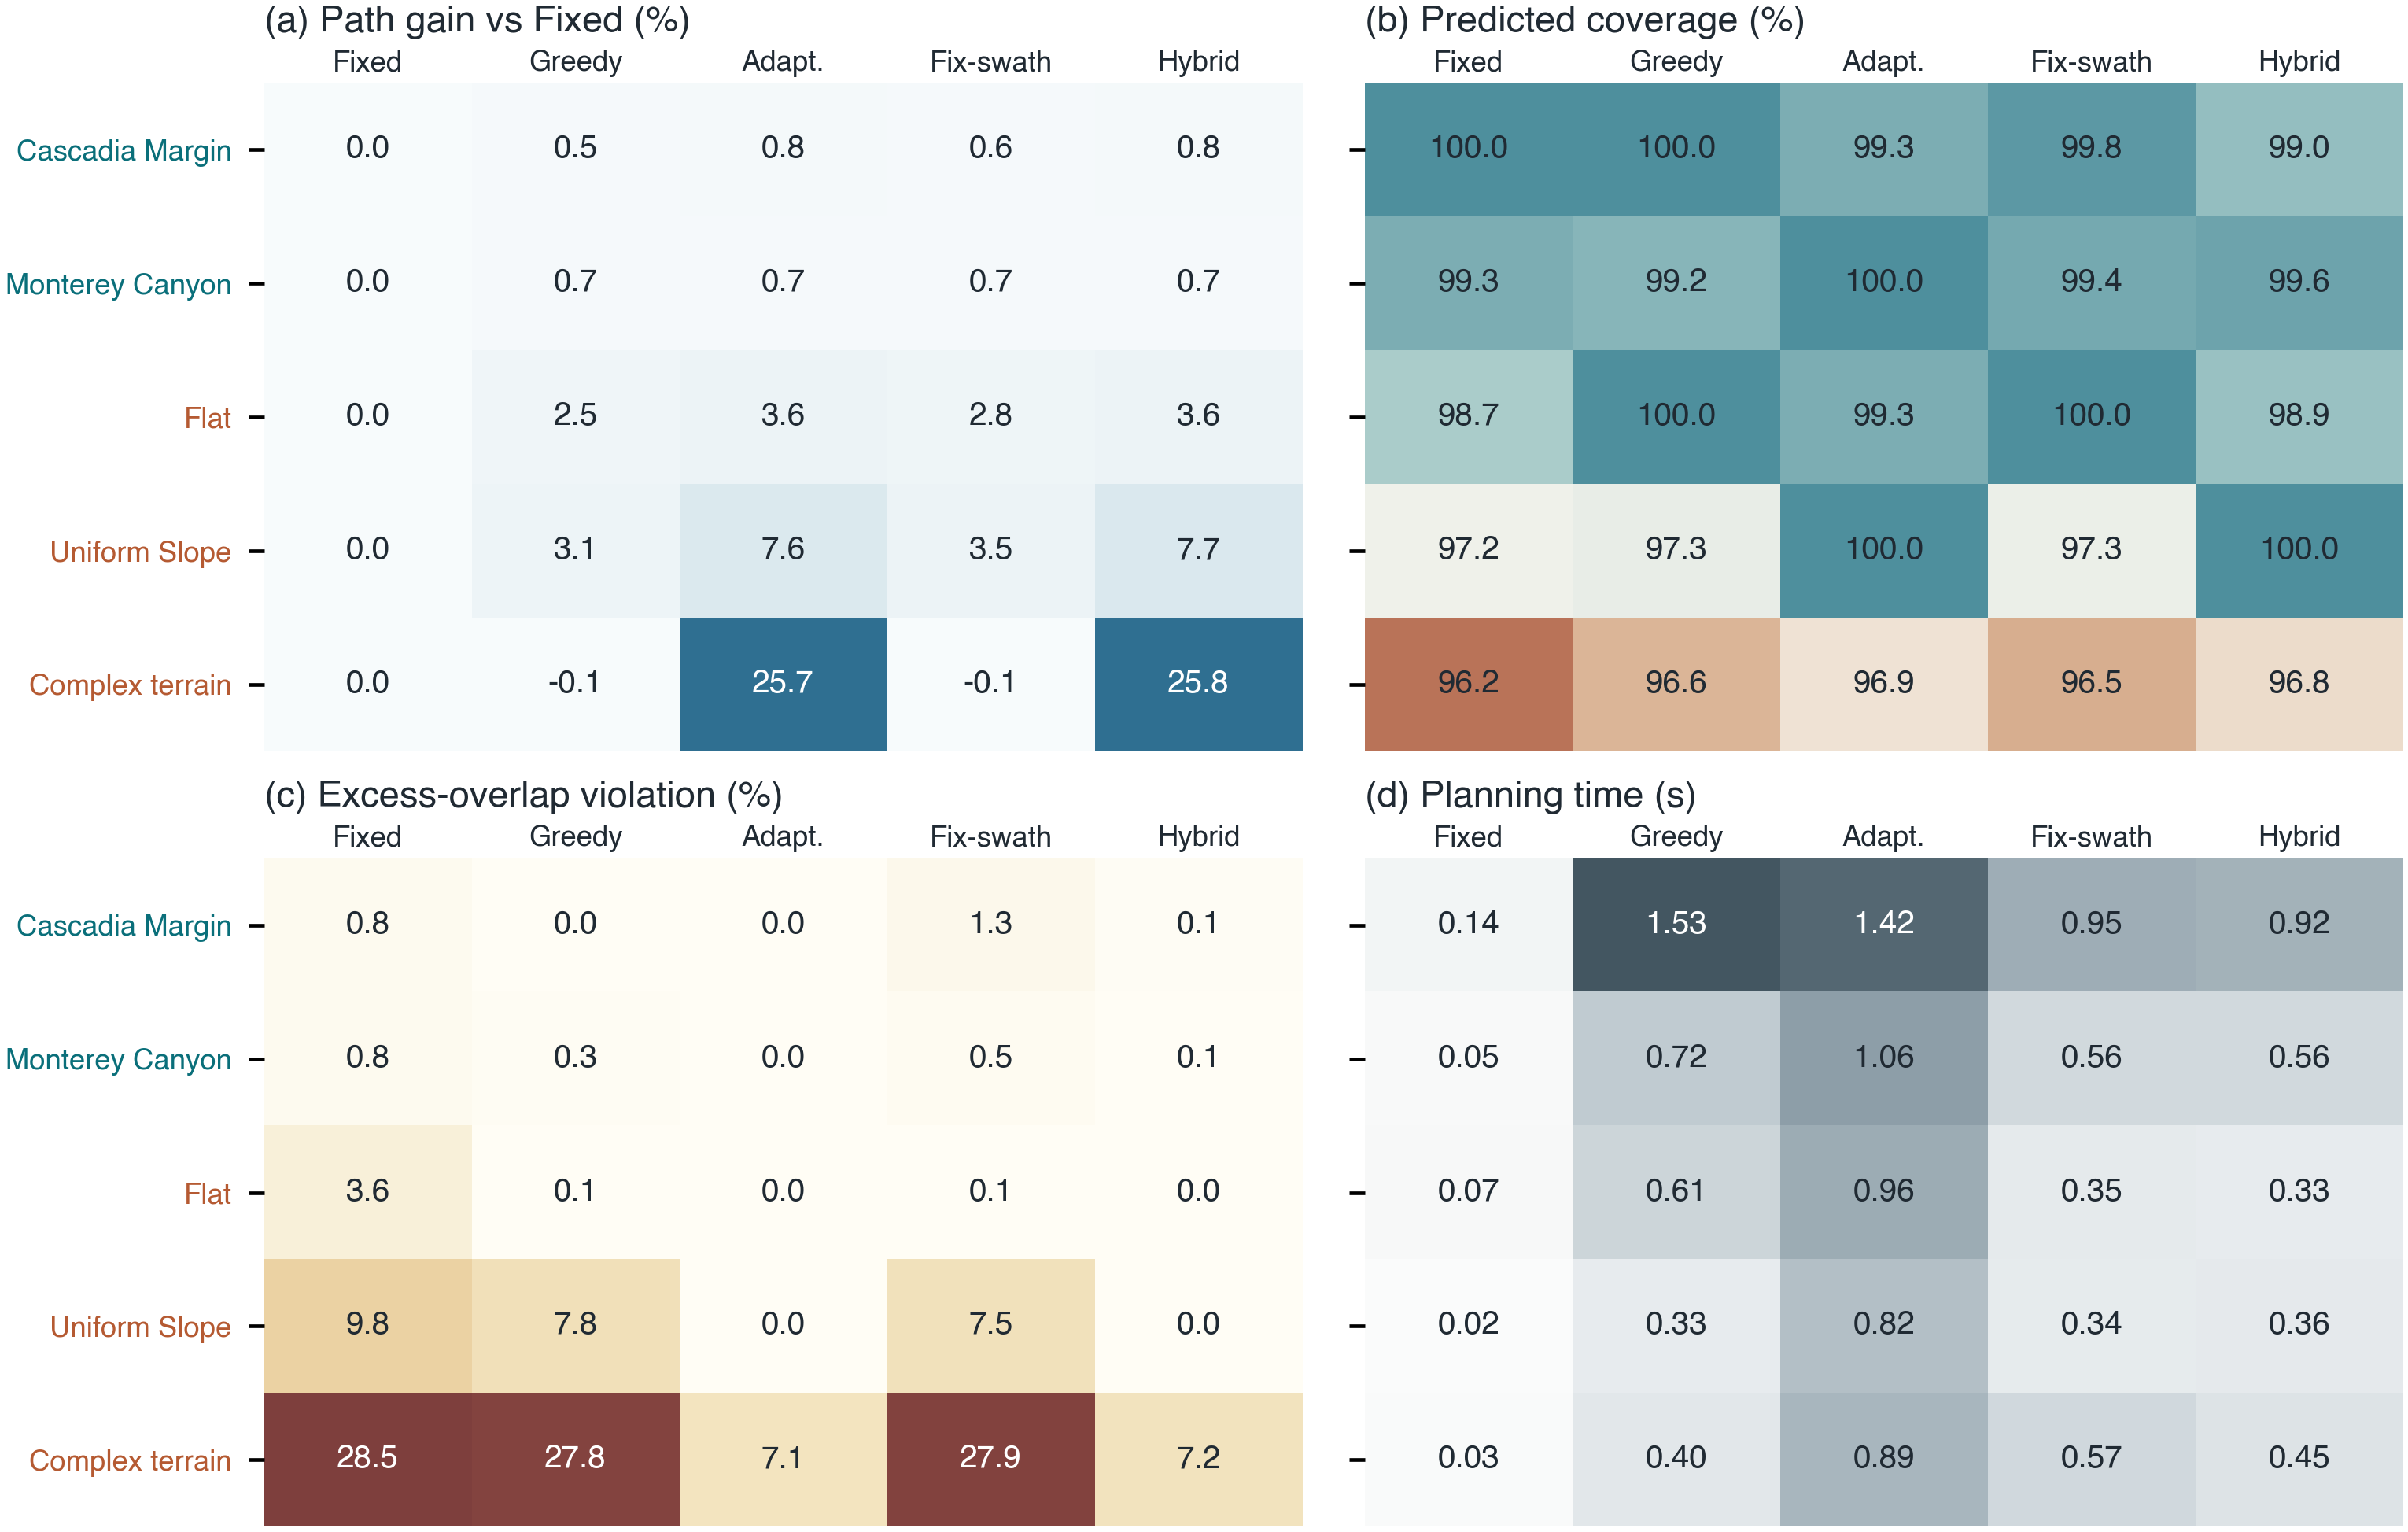
\includegraphics[width=\textwidth,height=0.36\textheight,keepaspectratio]{pic/journal_metric_heatmap.png}
	\caption{Cross-scene metric matrix from the reported benchmark. Each panel is a scene-by-method heatmap of benchmark means: path gain relative to Fixed-Spacing, predicted coverage, excess-overlap violation, and planning time. The top two rows are the public GEBCO scenes and the bottom three rows are synthetic stress tests, so the figure exposes both the public-data pattern and the complex-terrain failure boundary in one compact view. Stochastic GA methods report 50-seed means, and all coverage values are numerical predictions rather than field measurements.}
	\label{fig:results}
\end{figure}

Figure~\ref{fig:results} then lifts the argument from the two public cards to the full benchmark. First, the route-gain panel makes the terrain-heterogeneity effect explicit: the adaptive-only and hybrid methods deliver much larger relative savings on the synthetic scenes than on the public GEBCO subsets. Second, the coverage-margin panel shows why the Complex Terrain result is a failure case rather than a hidden success: the large path gain is accompanied by coverage below the 97 percent threshold. Third, the overlap panel shows that Fixed-Swath GA is not enough by itself; its path gain can be competitive, but its excess-overlap violation remains much larger than that of terrain-aware spacing. Fourth, the planning-time panel confirms that all tested methods remain in the offline-design regime for these benchmark sizes. Table~\ref{tab:all_scene_matrix} provides the corresponding compact numerical matrix for readers who need the exact cross-scene values behind the visual summary.

\begin{figure}[!htbp]
	\centering
	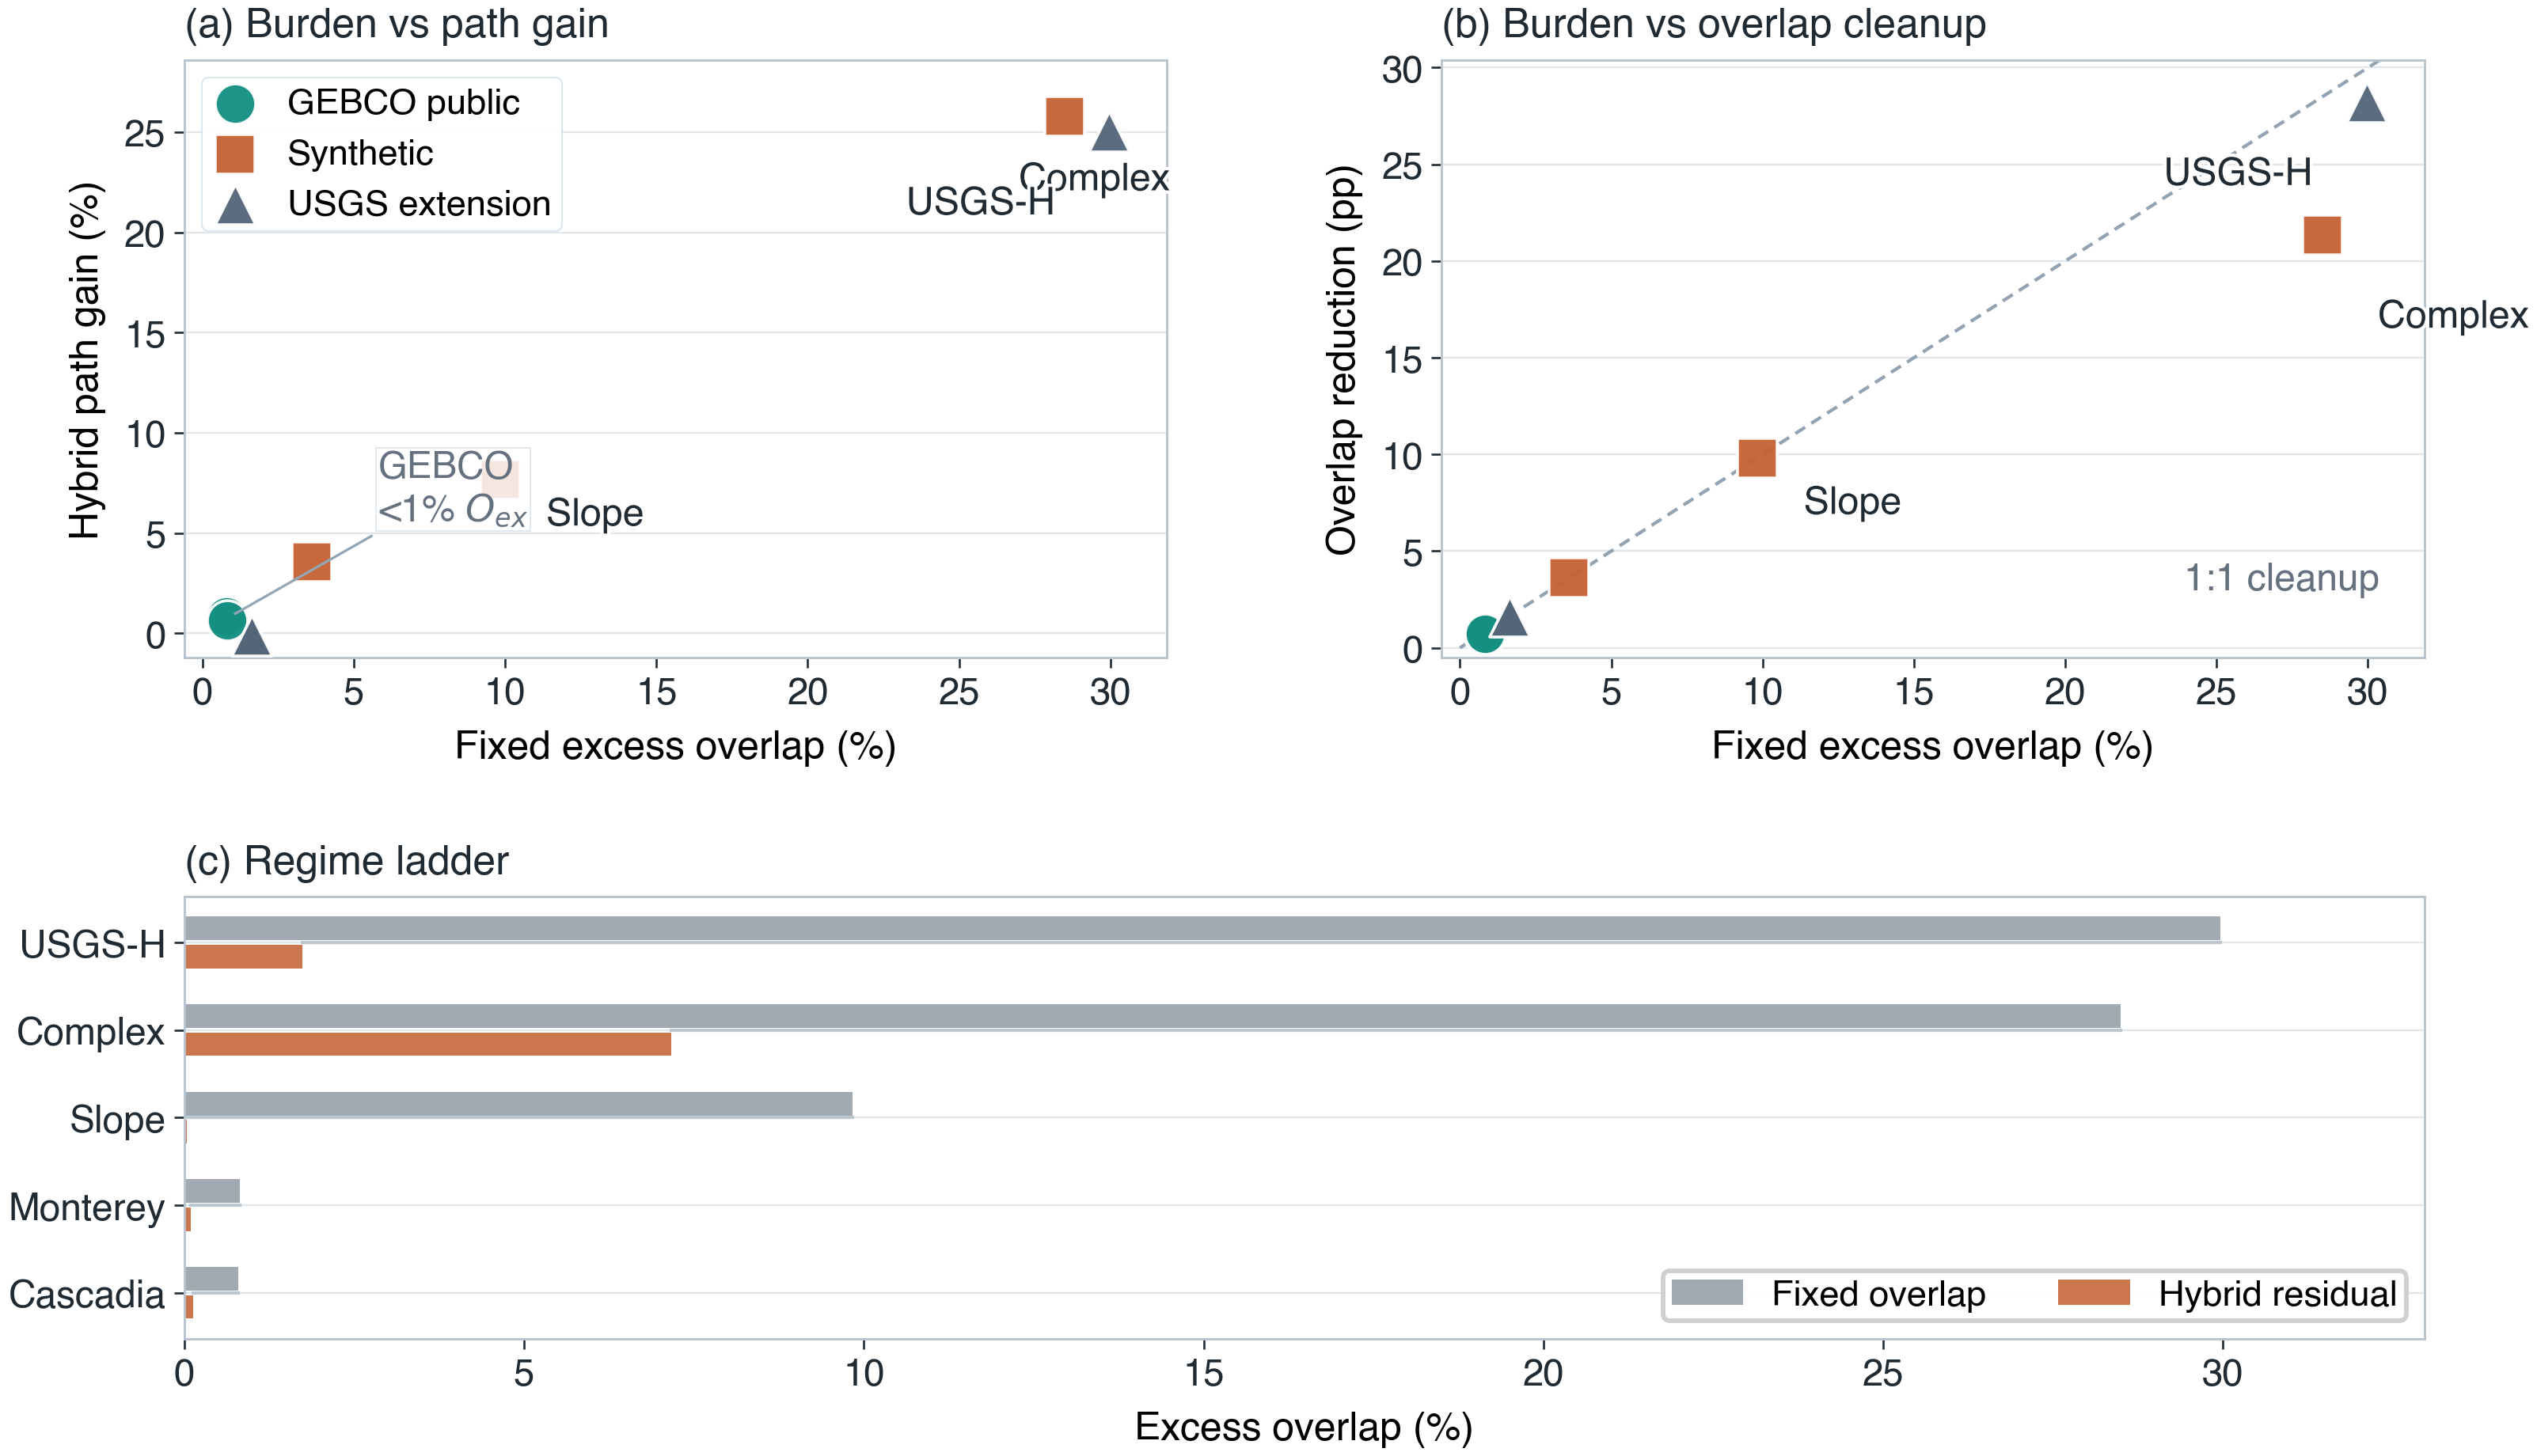
\includegraphics[width=0.96\textwidth,height=0.34\textheight,keepaspectratio]{pic/journal_overlap_regime.png}
	\caption{Scene-level regime diagnostic linking the Fixed-Spacing baseline to the observed Hybrid benefit. Each point is one scene from either the reported main benchmark or the separate USGS 30~m extension. Panel (a) plots Fixed-Spacing excess-overlap burden against Hybrid path gain relative to Fixed-Spacing. Panel (b) plots the same burden against Hybrid overlap reduction. Panel (c) gives a ranked overlap-regime ladder, comparing the Fixed-Spacing burden with the Hybrid residual on representative scenes. The GEBCO public scenes cluster in a low-overlap regime below 1 percent excess overlap, whereas Complex Terrain and the high-complexity USGS crop start near 30 percent excess overlap and therefore show the largest geometry-aware gains. The USGS points strengthen the mechanism interpretation but are not merged into the main benchmark averages reported elsewhere in the paper.}
	\label{fig:overlap_regime}
\end{figure}

Figure~\ref{fig:overlap_regime} makes the cross-scene mechanism more specific. Across the five benchmark scenes and the three USGS extension crops, the dominant predictor of terrain-aware benefit is not scene provenance by itself but the excess-overlap burden already present in the Fixed-Spacing baseline. The two GEBCO public scenes start at only 0.80 and 0.81 percent excess overlap and therefore yield only 0.66--0.85 percent route shortening, even though they still benefit from cleaner overlap control. The low- and medium-complexity USGS crops behave similarly: Fixed-Spacing already holds excess overlap at 1.633 percent, so terrain-aware spacing mainly removes that small surplus at negligible route-length cost. By contrast, Complex Terrain and the high-complexity USGS crop begin at 28.50 and 29.96 percent excess overlap and then deliver 25.77 and 25.07 percent path shortening, respectively, together with 21.32 and 28.21 percentage-point overlap cleanup. This pattern explains why the public gains are modest without weakening them: the reported GEBCO pair lives in a low-overlap regime rather than in the near-failure regime exposed by the harder synthetic scene and the high-complexity public-grid extension crop.

\begin{table}[!htbp]
	\centering
	\caption{Compact all-scene method matrix from the reported benchmark. Path gain is measured relative to Fixed-Spacing within the same scene. Coverage and excess overlap are reported in percent. Compact method labels abbreviate the five methods defined in the experimental protocol. Feasibility is the reported acceptance flag or, for stochastic methods, the mean feasibility rate over 50 seeds.}
	\label{tab:all_scene_matrix}
	\scriptsize
	\renewcommand{\arraystretch}{1.08}
	\setlength{\tabcolsep}{4.0pt}
	\begin{tabular}{@{}>{\raggedright\arraybackslash}p{0.19\linewidth}lrrrr@{}}
		\toprule[1bp]
		\textbf{Scene} & \textbf{Method} & \textbf{Gain (\%)} & \textbf{Coverage (\%)} & \textbf{Excess Overlap (\%)} & \textbf{Feas.} \\
		\midrule[1bp]
		\multirow{5}{*}{GEBCO Cascadia} & Fixed & 0.0 & 100.0 & 0.8 & 1.0 \\
		& Greedy & 0.5 & 100.0 & 0.0 & 1.0 \\
		& Adaptive without GA & 0.8 & 99.3 & 0.0 & 1.0 \\
		& Fixed-swath GA & 0.6 & 99.7 & 1.5 & 1.0 \\
		& Hybrid GA & 0.8 & 99.0 & 0.1 & 1.0 \\
		\midrule[0.5bp]
		\multirow{5}{*}{GEBCO Monterey} & Fixed & 0.0 & 99.3 & 0.8 & 1.0 \\
		& Greedy & 0.7 & 99.2 & 0.3 & 1.0 \\
		& Adaptive without GA & 0.7 & 100.0 & 0.0 & 1.0 \\
		& Fixed-swath GA & 0.7 & 99.5 & 0.5 & 1.0 \\
		& Hybrid GA & 0.7 & 99.6 & 0.1 & 1.0 \\
		\midrule[0.5bp]
		\multirow{5}{*}{Flat} & Fixed & 0.0 & 98.7 & 3.6 & 0.0 \\
		& Greedy & 2.5 & 100.0 & 0.1 & 1.0 \\
		& Adaptive without GA & 3.6 & 99.3 & 0.0 & 1.0 \\
		& Fixed-swath GA & 2.7 & 100.0 & 0.1 & 1.0 \\
		& Hybrid GA & 3.6 & 98.9 & 0.0 & 1.0 \\
		\midrule[0.5bp]
		\multirow{5}{*}{Uniform Slope} & Fixed & 0.0 & 97.2 & 9.8 & 0.0 \\
		& Greedy & 3.1 & 97.3 & 7.8 & 0.0 \\
		& Adaptive without GA & 7.6 & 100.0 & 0.0 & 1.0 \\
		& Fixed-swath GA & 3.6 & 97.3 & 7.5 & 0.0 \\
		& Hybrid GA & 7.7 & 100.0 & 0.0 & 1.0 \\
		\midrule[0.5bp]
		\multirow{5}{*}{Complex Terrain} & Fixed & 0.0 & 96.2 & 28.5 & 0.0 \\
		& Greedy & -0.1 & 96.6 & 27.8 & 0.0 \\
		& Adaptive without GA & 25.7 & 96.9 & 7.1 & 0.0 \\
		& Fixed-swath GA & -0.1 & 96.6 & 27.9 & 0.0 \\
		& Hybrid GA & 25.8 & 96.8 & 7.2 & 0.0 \\
		\bottomrule[1bp]
	\end{tabular}
\end{table}

The planning-time panel shows that runtime is not the dominant weakness of the present implementation. On the current workstation, all public-scene planners remained within about two seconds per scene, with Fixed-Spacing fastest and the terrain-aware planners still comfortably in the offline-planning regime. The method therefore remains limited primarily by modeling scope rather than by brute-force computational latency.

\subsection{Public-scene Ablation and Seed-level Repeatability}
Figure~\ref{fig:public_ablation_seed} isolates the two pieces of evidence most relevant to the public-data contribution claim: the ablation that separates adaptive spacing from GA refinement, and the seed-level dispersion of the Hybrid GA on the two public scenes.

\begin{figure}[!htbp]
	\centering
	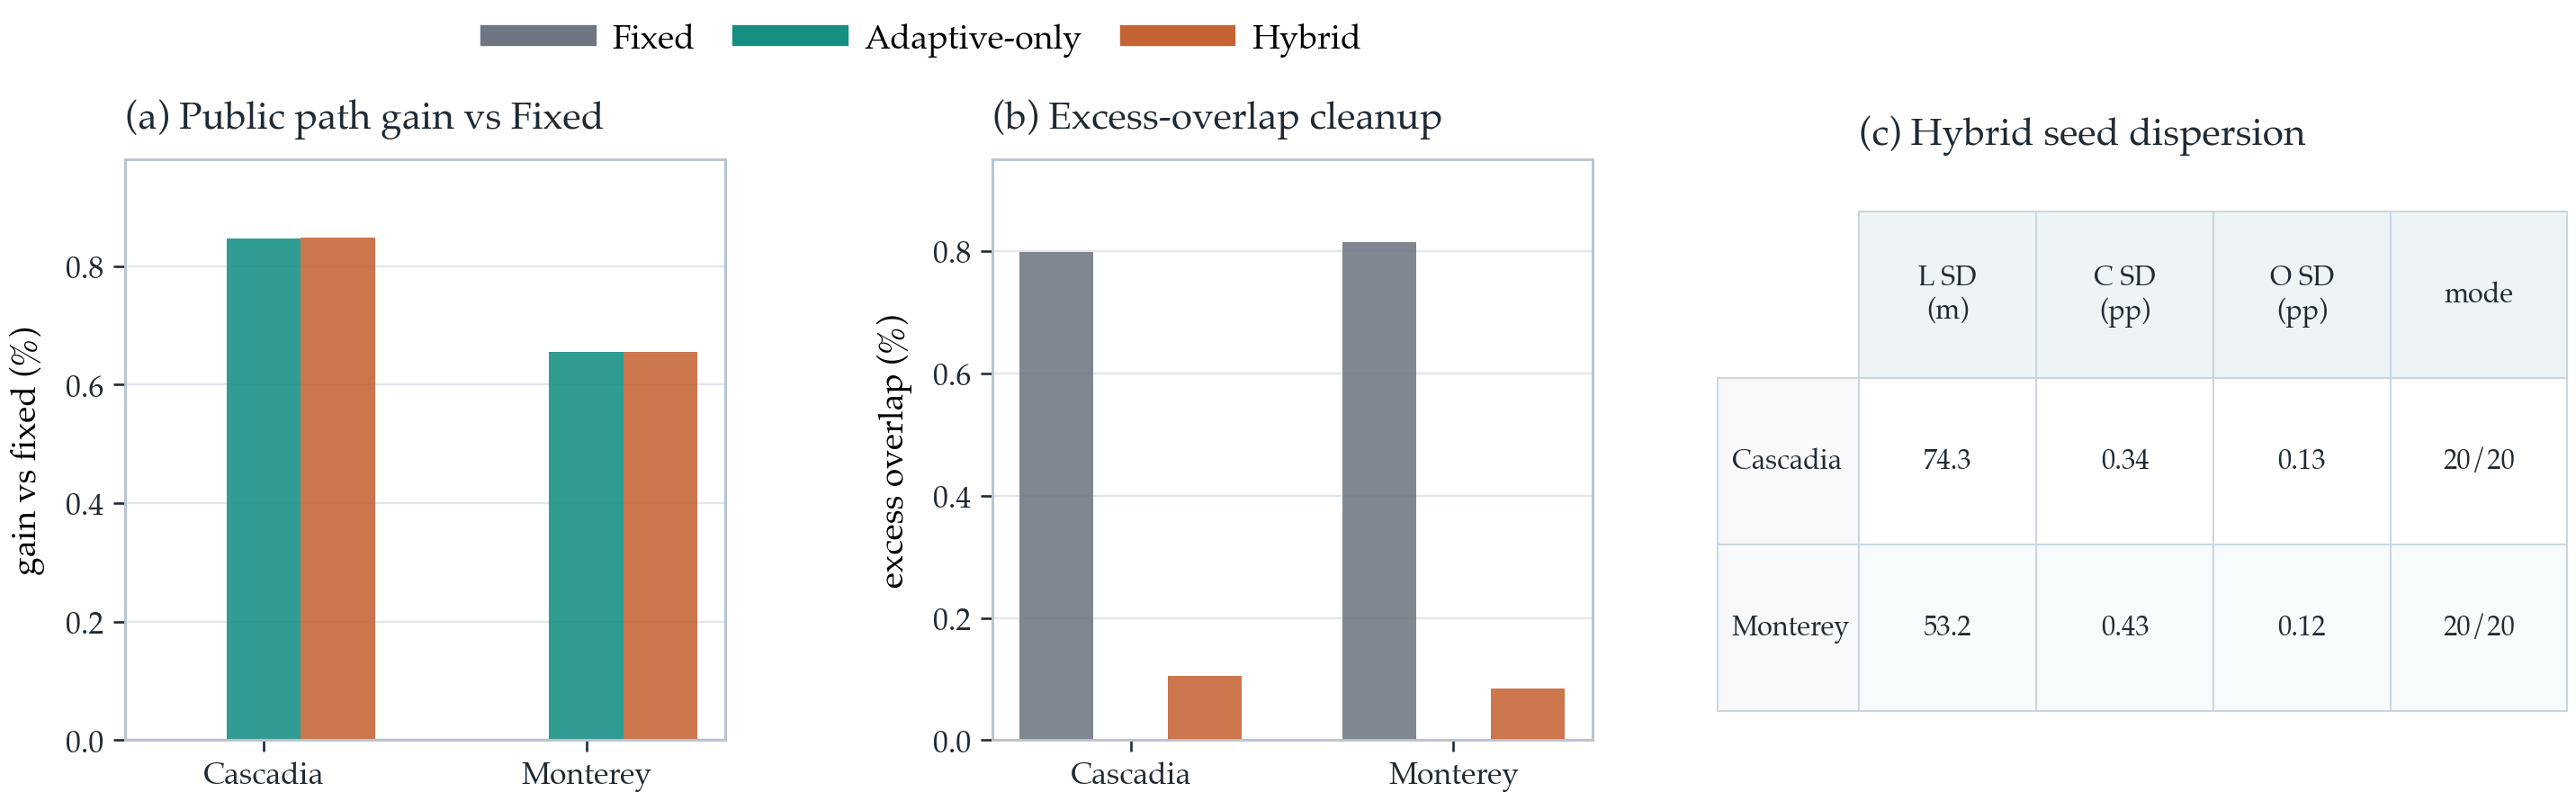
\includegraphics[width=\textwidth,height=0.36\textheight,keepaspectratio]{pic/journal_ablation_seed.png}
	\caption{Public-scene ablation and seed-level dispersion from the reported benchmark. Panels (a) and (b) compare Fixed-Spacing, Adaptive Spacing without GA, and Full Geometry-Aware Hybrid GA on path gain relative to Fixed-Spacing and on excess-overlap violation for the two public GEBCO scenes. Panel (c) reports the standard deviation of Hybrid GA path length \(L\), predicted coverage \(C\), and excess overlap \(O\) across 50 seeds, together with the count of seeds that converged to the dominant orientation/line-count mode.}
	\label{fig:public_ablation_seed}
\end{figure}

The main benchmark allows a direct 50-seed repeatability check on both public scenes. Table~\ref{tab:repeatability} shows that the Full Geometry-Aware Hybrid GA converged to the same heading mode and the same line-count mode in every seed: $0^{\circ}$/116 lines on GEBCO Cascadia Margin and $90^{\circ}$/59 lines on GEBCO Monterey Canyon. Path-length standard deviation stayed below 0.08~km, coverage standard deviation below 0.43 percentage points, and excess-overlap standard deviation below 0.15 percentage points. This is strong seed-level stability for the public-data benchmark, although it should not be confused with a full sensitivity characterization over hyperparameters, map quality, or execution uncertainty.

\begin{table}[!htbp]
	\centering
	\caption{Fifty-seed repeatability of the Full Geometry-Aware Hybrid GA on the two public GEBCO scenes from the reported benchmark. Heading and line-count modes were identical across all 50 seeds for each scene. Entries report mean $\pm$ standard deviation.}
		\label{tab:repeatability}
	\scriptsize
	\renewcommand{\arraystretch}{1.15}
		\resizebox{\textwidth}{!}{%
		\begin{tabular}{@{}lccccc@{}}
		\toprule[1bp]
		\textbf{Scene} & \textbf{Heading Mode} & \textbf{Line Count Mode} & \textbf{Path Length (km)} & \textbf{Coverage (\%)} & \textbf{Excess Overlap (\%)} \\
		\midrule[1bp]
		GEBCO Cascadia Margin & $0^{\circ}$ & 116 & 15038.15 $\pm$ 0.07 & 98.99 $\pm$ 0.34 & 0.14 $\pm$ 0.15 \\
		GEBCO Monterey Canyon & $90^{\circ}$ & 59 & 6656.57 $\pm$ 0.06 & 99.55 $\pm$ 0.42 & 0.09 $\pm$ 0.12 \\
		\bottomrule[1bp]
		\end{tabular}}
\end{table}

Table~\ref{tab:bootstrap_ci} adds a bootstrap confidence check over the same 50 Hybrid GA seeds. The deterministic Fixed-Spacing value is used only as the reference for gain and overlap cleanup; it is not treated as a random sample. The resulting intervals are intentionally reported as seed-level uncertainty, not as geographic or field-performance confidence intervals. They show that the modest public path gain is extremely stable under the present GA schedule, while the overlap-control conclusion remains positive even after accounting for seed-level dispersion.

\begin{table}[!htbp]
	\centering
	\caption{Seed-level bootstrap confidence intervals for the Full Geometry-Aware Hybrid GA on the public GEBCO scenes. Intervals are 95\% bootstrap CIs of the seed mean from 50 Hybrid GA runs and are recomputed from \texttt{run\_5/public\_hybrid\_bootstrap\_ci.csv}. \(G_L\) is path gain relative to the deterministic Fixed-Spacing layout; \(\Delta O\) is excess-overlap cleanup relative to Fixed-Spacing.}
	\label{tab:bootstrap_ci}
	\scriptsize
	\renewcommand{\arraystretch}{1.12}
	\resizebox{\textwidth}{!}{%
	\begin{tabular}{@{}lccccc@{}}
		\toprule[1bp]
		\textbf{Scene} & \textbf{Feasible seeds} & \textbf{\(G_L\) mean [95\% CI] (\%)} & \textbf{Coverage mean [95\% CI] (\%)} & \textbf{Excess overlap mean [95\% CI] (\%)} & \textbf{\(\Delta O\) mean [95\% CI] (pp)} \\
		\midrule[1bp]
		GEBCO Cascadia Margin & 50/50 & 0.8476 [0.8475, 0.8477] & 98.9867 [98.8933, 99.0800] & 0.1353 [0.0970, 0.1783] & 0.6632 [0.6198, 0.7013] \\
		GEBCO Monterey Canyon & 50/50 & 0.6559 [0.6557, 0.6562] & 99.5500 [99.4333, 99.6667] & 0.0903 [0.0607, 0.1232] & 0.7245 [0.6916, 0.7545] \\
		\bottomrule[1bp]
	\end{tabular}}
\end{table}

The repeatability and bootstrap results show strong seed-level stability on the public-data benchmark. The claim remains limited to the current configuration and does not amount to a full sensitivity analysis across GA settings, bathymetry resolution, spatially varying prior-map mismatch, or uncertainty margins.

\subsection{Adaptive-vs-Hybrid Practical Significance and Gate Diagnostic}
Table~\ref{tab:ga_gate_practical} reports the submission-boundary diagnostic that compares 20 raw Hybrid GA seeds with the deterministic Adaptive Spacing baseline at the reported \(W_{\max}=1800~\mathrm{m}\). The table intentionally avoids p-value inflation: it reports paired practical deltas, score-better rates, and how often the conservative operational gate would accept the raw GA refinement rather than falling back to Adaptive Spacing.

\begin{table}[!htbp]
	\centering
	\caption{Adaptive-vs-Hybrid practical-significance and operational-gate diagnostic at \(W_{\max}=1800~\mathrm{m}\). Positive path gain means Hybrid GA is shorter than Adaptive Spacing; positive \(\Delta C\) means higher predicted coverage; positive \(\Delta O\) means higher mean excess overlap and is therefore worse. The gate accepts a raw Hybrid seed only when it remains feasible, is no worse than Adaptive by 0.05 percentage points in coverage and overlap, and is no longer in path length.}
	\label{tab:ga_gate_practical}
	\scriptsize
	\renewcommand{\arraystretch}{1.10}
	\resizebox{\textwidth}{!}{%
	\begin{tabular}{@{}lrrrrr@{}}
		\toprule[1bp]
		\textbf{Scene} & \textbf{Median path gain vs. Adaptive (\%)} & \textbf{Median \(\Delta C\) (pp)} & \textbf{Median \(\Delta O\) (pp)} & \textbf{Score-better seeds} & \textbf{Gate-accepted seeds} \\
		\midrule[1bp]
		GEBCO Cascadia Margin & 0.0003 & -0.6667 & 0.0750 & 2/20 & 7/20 \\
		GEBCO Monterey Canyon & 0.0004 & 0.0000 & 0.0219 & 2/20 & 8/20 \\
		USGS High-complexity crop & 1.3684 & -0.1167 & -0.5157 & 20/20 & 6/20 \\
		\bottomrule[1bp]
	\end{tabular}}
\end{table}

The diagnostic confirms the intended role of GA. On the two GEBCO public-prior scenes, the median path gain of raw Hybrid GA over Adaptive Spacing is below \(0.001\%\), while the median coverage or overlap delta is often slightly worse; only 2 of 20 seeds improve the declared score. A conservative gate would therefore retain the deterministic adaptive layout for most GEBCO seeds. On the USGS high-complexity crop, raw Hybrid GA is more useful: the median path gain is 1.37\% and median excess overlap improves by 0.516 percentage points relative to Adaptive Spacing, although the median coverage delta is \(-0.117\) percentage points and the gate accepts only 6 of 20 seeds. This supports a procedural interpretation: use Adaptive Spacing as the deterministic baseline, then accept local GA cleanup only when a declared gate confirms that the route improvement is not bought by worse coverage or overlap.

Table~\ref{tab:ga_surrogate_audit} adds the corresponding stride-3 surrogate audit. The audit samples 144 local line-position perturbations per scene around the Adaptive Spacing base layout, ranks them by the same stride-3 GA fitness used during refinement, and then rescors each candidate on the full evaluator grid. The high rank correlations and low full-grid regret show that the subsampled fitness is adequate for local screening in the tested scenes. This does not eliminate the need for full-grid final reporting, but it reduces the risk that the GA is being guided by a materially different evaluator.

\begin{table}[!htbp]
	\centering
	\caption{GA surrogate audit comparing stride-3 fitness ranking with full-grid rescoring for local perturbations around the deterministic Adaptive Spacing layout. Each scene uses 12 seeds and 12 sampled candidates per seed. Spearman and Kendall values compare the stride-3 and full-grid GA-fitness rankings; top-10 overlap reports the fraction of the ten best stride-ranked candidates that are also among the ten best full-grid candidates; regret is the full-grid score gap between the stride-selected candidate and the best full-grid candidate in the sampled local cloud.}
	\label{tab:ga_surrogate_audit}
	\scriptsize
	\renewcommand{\arraystretch}{1.08}
	\resizebox{\textwidth}{!}{%
	\begin{tabular}{@{}lrrrrr@{}}
		\toprule[1bp]
		\textbf{Scene} & \textbf{Candidates} & \textbf{Spearman} & \textbf{Kendall \(\tau\)} & \textbf{Top-10 overlap} & \textbf{Full-grid regret (\%)} \\
		\midrule[1bp]
		GEBCO Cascadia Margin & 144 & 0.934 & 0.804 & 0.80 & 0.0008 \\
		GEBCO Monterey Canyon & 144 & 0.968 & 0.855 & 0.70 & 0.0028 \\
		USGS High-complexity crop & 144 & 0.989 & 0.920 & 0.80 & 0.0610 \\
		\bottomrule[1bp]
	\end{tabular}}
\end{table}

\subsection{External Optimizer Sanity Check}
To check whether the public result depends narrowly on choosing GA as the local search operator, we added an equal-budget Particle Swarm Optimization (PSO) diagnostic on the two public GEBCO scenes. The PSO variant starts from the same Adaptive Spacing baseline as the Hybrid GA, keeps the same heading and line count, and refines only cross-track positions with 10 particles and 10 iterations. This makes it a like-for-like local-refinement sanity check rather than a new global CPP competitor. The diagnostic uses seeds 0--9 and does not replace the 50-seed Hybrid GA benchmark reported above. Because the PSO check is a secondary optimizer-dependence test rather than a main evidence pillar, the detailed bar plot is retained in the reproducibility package instead of being promoted as another main-text figure.

The PSO check supports the interpretation that terrain-aware spacing, not a particular metaheuristic label, is the main source of the public-scene path shortening. PSO produced comparable or slightly shorter path lengths, with 0.848 percent and 0.657 percent path gain on Cascadia and Monterey, respectively. However, it also produced lower predicted coverage than Hybrid GA in this diagnostic and higher residual excess overlap: 0.150 percent versus 0.089 percent on Cascadia, and 0.126 percent versus 0.059 percent on Monterey. The result therefore sharpens the claim rather than inflating it. The stochastic refinement step can be implemented by more than one local optimizer, but none of these equal-budget local refinements changes the main conclusion that deterministic terrain-aware spacing carries the public-scene benefit.

\subsection{External Survey-layout Heuristic Audit}
To further address the concern that all main baselines are drawn from the same fixed-pattern family, we added a compact external heuristic audit on the nine public-grid windows. The audit implements three deterministic rules that are common in survey-layout reasoning but do not use the proposed adaptive-spacing profile: a minimum-span boustrophedon heading, a contour-parallel fixed-width heading estimated from the dominant terrain-gradient direction, and a geometry-shortest fixed-width heading. All three use the same scene-wide \(q=0.30\) swath-width spacing rule and are then scored by the same coverage, overlap, and path evaluator as the main methods. This is not a reproduction of a full vehicle-dynamics, multi-objective, or field-validated CPP system; its purpose is to add an external-style layout sanity check without changing the benchmark scope.

Table~\ref{tab:external_layout_audit} summarizes the result. The external heuristics are competitive on several low-overlap GEBCO windows, and the geometry-shortest fixed-width rule passes the default \(C97/O3\) gate in 8 of 9 public windows. The stress case remains decisive: on the USGS high-complexity crop, all three fixed-width external heuristics fail the default gate because their coverage drops to about 92.4--92.6 percent or their mean excess overlap remains 7.49--15.34 percent. Adaptive Spacing and the representative seed-0 Hybrid layout pass all nine public windows in this audit, with median path gains of 0.681 percent and median excess-overlap values of 0.000 percent. The table therefore strengthens the bounded claim: the paper is not asserting global superiority over all CPP planners, but the proposed terrain-aware spacing layer is more reliable than simple geometry-only fixed-width heuristics under the reported public-grid evaluator.

\begin{table}[!htbp]
	\centering
	\caption{External survey-layout heuristic audit on nine public-grid windows. External heuristics are deterministic fixed-width line-layout rules scored by the same evaluator as the main benchmark; Hybrid uses seed 0 only in this audit, whereas the main benchmark reports 50 seeds. Feasibility uses the default \(C97/O3\) gate.}
	\label{tab:external_layout_audit}
	\scriptsize
	\renewcommand{\arraystretch}{1.08}
	\setlength{\tabcolsep}{3.4pt}
	\resizebox{\textwidth}{!}{%
	\begin{tabular}{@{}lrrrrr@{}}
		\toprule[1bp]
		\textbf{Method} & \textbf{Feasible windows} & \textbf{Median path gain (\%)} & \textbf{Median coverage (\%)} & \textbf{Median \(O_{\mathrm{ex}}\) (\%)} & \textbf{Median cleanup (pp)} \\
		\midrule[1bp]
		Min-span boustrophedon & 6/9 & 0.350 & 99.17 & 0.801 & 0.126 \\
		Contour-parallel fixed-width & 6/9 & 0.128 & 99.99 & 0.439 & 0.619 \\
		Geometry-shortest fixed-width & 8/9 & 0.398 & 99.99 & 0.226 & 0.514 \\
		Adaptive Spacing without GA & 9/9 & 0.681 & 99.33 & 0.000 & 0.799 \\
		Hybrid GA seed 0 & 9/9 & 0.681 & 99.33 & 0.000 & 0.781 \\
		\bottomrule[1bp]
	\end{tabular}}
\end{table}

\subsection{External Heuristic Turning-cost Audit}
The external heuristic audit above still reports geometric line length. To address the reviewer concern that fixed-line layouts may change rank once line-change maneuvers are considered, we added a deterministic turning-cost post-evaluation on the same 54 scene--method rows. For each layout, the audit adds a semicircular line-change penalty \((N-1)\pi R_{\min}\), evaluates \(R_{\min}=25,50,100,\) and \(200\)~m, and converts the geometric path plus turn arcs into a mission-time proxy using 1.5~m~s\(^{-1}\) for survey/transit distance and 0.75~m~s\(^{-1}\) for turn arcs. Coverage and overlap are not recomputed because the line family is unchanged. The diagnostic is therefore a post-planning execution-cost screen, not a Dubins controller, hydrodynamic model, mission-log replay, or field validation.

Table~\ref{tab:external_turning_cost_audit} shows that the turning-cost proxy does not reverse the bounded conclusion from Table~\ref{tab:external_layout_audit}. At \(R_{\min}=100\)~m, Adaptive Spacing and Hybrid seed 0 remain feasible in all nine public windows and retain a median mission-time gain of 0.682 percent relative to Fixed-Spacing. The geometry-shortest fixed-width heuristic is competitive in median time gain, but passes only 8 of 9 windows. The USGS high-complexity crop explains why the gate must be read together with the time metric: Min-span and Geometry-shortest fixed-width show a large \(R_{\min}=100\) mission-time gain of 37.83 percent on that crop, but both remain infeasible because predicted coverage is only 92.44 percent and mean excess overlap is 7.49 percent. By contrast, Adaptive Spacing and Hybrid seed 0 remain feasible on the same crop, with \(R_{\min}=100\) mission-time gains of 22.43 and 23.41 percent. The audit therefore strengthens the operational interpretation without upgrading the claim to execution validation: a shorter or faster fixed-width sweep is not useful if it fails the declared coverage/overlap gate.

\begin{table}[!htbp]
	\centering
	\caption{External heuristic turning-cost audit on the same nine public-grid windows as Table~\ref{tab:external_layout_audit}. Mission-time gain adds semicircular line-change arcs and a slower turn speed to the geometric path; feasibility is still the unchanged \(C97/O3\) coverage/overlap gate.}
	\label{tab:external_turning_cost_audit}
	\scriptsize
	\renewcommand{\arraystretch}{1.12}
	\setlength{\tabcolsep}{4.2pt}
	\begin{tabular}{@{}lrrrrrr@{}}
		\toprule[1bp]
		\textbf{Method} & \textbf{Feas.} & \textbf{R100 gain} & \textbf{R100 +} & \textbf{R200 gain} & \textbf{R200 +} & \textbf{Turn share} \\
		& & \textbf{(\%)} & & \textbf{(\%)} & & \textbf{R100 (\%)} \\
		\midrule[1bp]
		Min-span boustrophedon & 6/9 & 0.654 & 8/9 & 0.787 & 8/9 & 0.173 \\
		Contour-parallel fixed-width & 6/9 & 0.050 & 5/9 & 0.000 & 4/9 & 0.219 \\
		Geometry-shortest fixed-width & 8/9 & 0.434 & 7/9 & 0.471 & 7/9 & 0.194 \\
		Adaptive Spacing without GA & 9/9 & 0.682 & 7/9 & 0.682 & 7/9 & 0.240 \\
		Hybrid GA seed 0 & 9/9 & 0.682 & 7/9 & 0.682 & 7/9 & 0.240 \\
		\bottomrule[1bp]
	\end{tabular}
\end{table}

\subsection{Sensitivity to Declared Sensor, Map, and Planning Inputs}
Table~\ref{tab:sensitivity_diagnostics} summarizes the additional public-scene diagnostics around the main benchmark. These diagnostics make the numerical claim harder to dismiss as a single-parameter artifact by testing sensor aperture, design margin, prior-map perturbation, objective weighting, and public-grid resolution around the same reported layouts. Across \(100^{\circ}\)--\(130^{\circ}\) MBES opening-angle reruns, the Hybrid GA retained the same public-scene heading and line-count modes as the main benchmark: \(0^{\circ}\)/116 lines on Cascadia and \(90^{\circ}\)/59 lines on Monterey, with all tested runs feasible in the 20-seed diagnostic. This result should be interpreted as a local sensor-parameter check under the same idealized footprint model, not as a calibration study of real sonar performance.

\begin{table}[!htbp]
	\centering
	\caption{Public-scene sensitivity diagnostics around the main benchmark. Hybrid GA summaries use seeds 0--19 for the sensitivity diagnostics, whereas the main reported benchmark uses 50 seeds.}
	\label{tab:sensitivity_diagnostics}
	\scriptsize
	\renewcommand{\arraystretch}{1.12}
	\setlength{\tabcolsep}{3.0pt}
	\begin{tabular}{@{}>{\raggedright\arraybackslash}p{0.17\linewidth}>{\raggedright\arraybackslash}p{0.19\linewidth}>{\raggedright\arraybackslash}p{0.32\linewidth}>{\raggedright\arraybackslash}p{0.18\linewidth}@{}}
		\toprule[1bp]
		\textbf{Diagnostic} & \textbf{Values tested} & \textbf{Observed public-scene outcome} & \textbf{Remaining boundary} \\
		\midrule[1bp]
		MBES opening angle & \(100^{\circ}\), \(110^{\circ}\), \(120^{\circ}\), \(130^{\circ}\) & Hybrid GA kept the same heading and line-count modes on both public scenes; 20-seed feasibility stayed 1.0, with mean predicted coverage of 98.97\% on Cascadia and 99.63\% on Monterey. & Local idealized-footprint check, not sonar calibration or field-performance evidence. \\
		Heading resolution & \(15^{\circ}\) main scan; \(5^{\circ}\) diagnostic for Simple Greedy and Adaptive Spacing & Adaptive Spacing selected the same headings and metrics on Cascadia, Monterey, and the USGS high-complexity crop. Simple Greedy changed only on Cascadia, from \(75^{\circ}\) to \(95^{\circ}\), shortening the route by 0.123\% while increasing mean excess overlap by 0.084 pp. & Supports the reported \(15^{\circ}\) benchmark; final deployment could still use a coarse-to-fine heading refinement. \\
		Target-overlap margin & 10\%, 15\%, 20\% & All tested public layouts remained feasible, but selected headings and line counts changed across margins. & The margin is a declared design parameter, not a universal constant. \\
		Public-grid resolution & native, \(2\times\), \(3\times\) stride & Cascadia remained feasible across tested strides; Monterey Hybrid GA became marginal at \(3\times\) stride with mean coverage near 97.56\% and feasibility rate 0.95. & Coarse public grids can erode evaluated coverage margin. \\
		Simple prior-map perturbation & depth bias \(\pm150\)~m; relief scale 0.7--1.3 & Public-scene headings, line counts, and reported means were unchanged under these global perturbations. & Does not test spatially structured map error or navigation drift. \\
		Objective penalty weights & coverage penalty 40, 80, 160; overlap penalty 1.5, 3.0, 6.0 & Public-scene headings and line counts stayed unchanged across the \(3\times3\) grid; Hybrid GA path-gain ranges were 0.8474--0.8476\% on Cascadia and 0.6551--0.6574\% on Monterey. & Objective-weight diagnostic only; it does not replace broader multi-objective tuning. \\
		\bottomrule[1bp]
	\end{tabular}
\end{table}

Table~\ref{tab:wmax_sensitivity} reports the additional swath-cap diagnostic requested for the submission package. The cap changes absolute line density and path totals substantially, so it should be read as a declared evaluator parameter rather than as a hidden physical sonar truth. The tested caps do not overturn the low-overlap interpretation of the two GEBCO scenes, but the USGS high-complexity crop fails the default overlap gate when \(W_{\max}\) is relaxed to 2400~m, showing that cap selection is material in overlap-stressed terrain.

\begin{table}[!htbp]
	\centering
	\caption{Submission-boundary sensitivity to the declared upper swath-width cap. Values are Hybrid GA 20-seed means for the two primary GEBCO scenes and the USGS high-complexity crop. \(F\) is the default \(C97/O3\) feasibility rate; \(L\), \(C\), and \(O\) denote path length, predicted coverage, and mean excess-overlap violation.}
	\label{tab:wmax_sensitivity}
	\scriptsize
	\renewcommand{\arraystretch}{1.08}
	\resizebox{\textwidth}{!}{%
	\begin{tabular}{@{}lrrrrrr@{}}
		\toprule[1bp]
		\textbf{Scene} & \textbf{\(W_{\max}\) (m)} & \textbf{\(F\)} & \textbf{\(L\) (km)} & \textbf{\(C\) (\%)} & \textbf{\(O\) (\%)} & \textbf{Lines} \\
		\midrule[1bp]
		GEBCO Cascadia Margin & 1200 & 1.00 & 22528.10 & 99.84 & 1.214 & 166.0 \\
		GEBCO Cascadia Margin & 1800 & 1.00 & 15038.16 & 98.97 & 0.106 & 116.0 \\
		GEBCO Cascadia Margin & 2400 & 1.00 & 11322.07 & 99.10 & 0.104 & 87.0 \\
		GEBCO Monterey Canyon & 1200 & 1.00 & 9884.86 & 98.58 & 0.248 & 88.0 \\
		GEBCO Monterey Canyon & 1800 & 1.00 & 6656.57 & 99.63 & 0.085 & 59.0 \\
		GEBCO Monterey Canyon & 2400 & 1.00 & 4983.59 & 98.33 & 0.025 & 54.0 \\
		USGS High-complexity crop & 1200 & 1.00 & 84.48 & 98.81 & 1.049 & 12.0 \\
		USGS High-complexity crop & 1800 & 1.00 & 72.90 & 98.44 & 1.732 & 12.0 \\
		USGS High-complexity crop & 2400 & 0.00 & 73.00 & 98.81 & 6.391 & 12.0 \\
		\bottomrule[1bp]
	\end{tabular}}
\end{table}

The target-overlap diagnostic is best read as a discrete design-margin check, not as a continuous trend. All tested settings remain feasible on both GEBCO scenes, so the main conclusion that terrain-aware spacing can control overlap while preserving predicted coverage is not limited to the 15 percent target-overlap value. The selected layout, however, is not invariant to this design margin. On Cascadia, the adaptive and hybrid planners switch between $90^{\circ}$ layouts at the 10 percent and 20 percent settings and the $0^{\circ}$ layout used in the main benchmark configuration at 15 percent. On Monterey, the 10 percent setting selects a $75^{\circ}$ adaptive family, the 15 percent setting selects the main $90^{\circ}$ family, and the 20 percent setting returns to a denser $0^{\circ}$ family. This sensitivity is not a failure of the benchmark, but it means that the overlap margin should be treated as a declared planning parameter rather than as a universal constant; the full target-overlap evidence matrix is retained with the reproducibility artifacts.

The grid-resolution diagnostic adds a second boundary check. On Cascadia, the terrain-aware line family remains feasible under native, \(2\times\), and \(3\times\) strided grids, although coverage margin decreases from the native value as the grid is coarsened. Monterey is more sensitive. The adaptive-only planner remains feasible and holds predicted coverage at 100.0 percent in the downsampled diagnostic, but the Hybrid GA mean drops to 97.56 percent coverage at the \(3\times\) stride and the feasibility rate falls to 0.95 across seeds 0--19. This does not overturn the main native-grid result; it shows that the public benchmark is resolution dependent and that coarse bathymetric products can reduce the safety margin of the evaluated fixed-line family. The full grid-resolution matrix is kept as supplementary/reproducibility evidence rather than occupying a separate main-text figure page.

The supplementary prior-depth-bias and relief-scale checks test a simpler form of prior-map sensitivity. Rerunning the planners on a uniformly depth-biased prior (\(\pm 150\)~m) and on relief-scaled priors (0.7, 1.0, 1.3) left the public-scene layouts unchanged on Cascadia and Monterey: the dominant orientations and line-count modes stayed fixed, and the coverage, excess-overlap, and path-gain means were numerically unchanged. A separate objective-weight diagnostic reran the public scenes across a \(3\times3\) coverage/overlap penalty grid and likewise retained the same selected line-family modes for the reported methods. The result does not make the weights universal, but it reduces the risk that the public result is a single penalty-weight artifact. This rules out trivial global prior offsets and local weight choices as the explanation for the public-scene result while motivating separate structured prior-error and execution-noise replays for spatially varying uncertainty.

The \(5^{\circ}\) heading-resolution diagnostic addresses a smaller but important quantization objection. For Adaptive Spacing, the \(5^{\circ}\) rerun exactly reproduced the \(15^{\circ}\) selected headings and metrics on GEBCO Cascadia, GEBCO Monterey, and the USGS high-complexity crop. For Simple Greedy, only Cascadia changed, from \(75^{\circ}\) to \(95^{\circ}\), reducing path length by 0.123\% and increasing mean excess overlap by 0.084 percentage points while preserving feasibility. The main public conclusion is therefore not an artifact of a coarse heading grid: the terrain-aware adaptive base used by Hybrid GA is invariant in this audit, and the only detected constant-spacing shift is smaller than the reported public overlap-cleanup effect. The full CSV, JSON, and compact diagnostic PNG are kept in the reproducibility package rather than added as another main-text figure.

\subsection{Structured Prior-error Replay}
Figure~\ref{fig:structured_prior_error} adds a stronger prior-map robustness check than the uniform depth-bias diagnostic. In this replay, each planner is given a spatially erroneous prior and the selected line family is then evaluated on the unperturbed truth grid. The tested perturbations are intentionally structured: a low-frequency correlated bias, a slope-amplified correlated error, and a localized canyon-wall bias. The replay therefore asks whether the line-layout decision survives map error with spatial shape, rather than only a global offset or relief scaling.

\begin{figure}[!htbp]
	\centering
	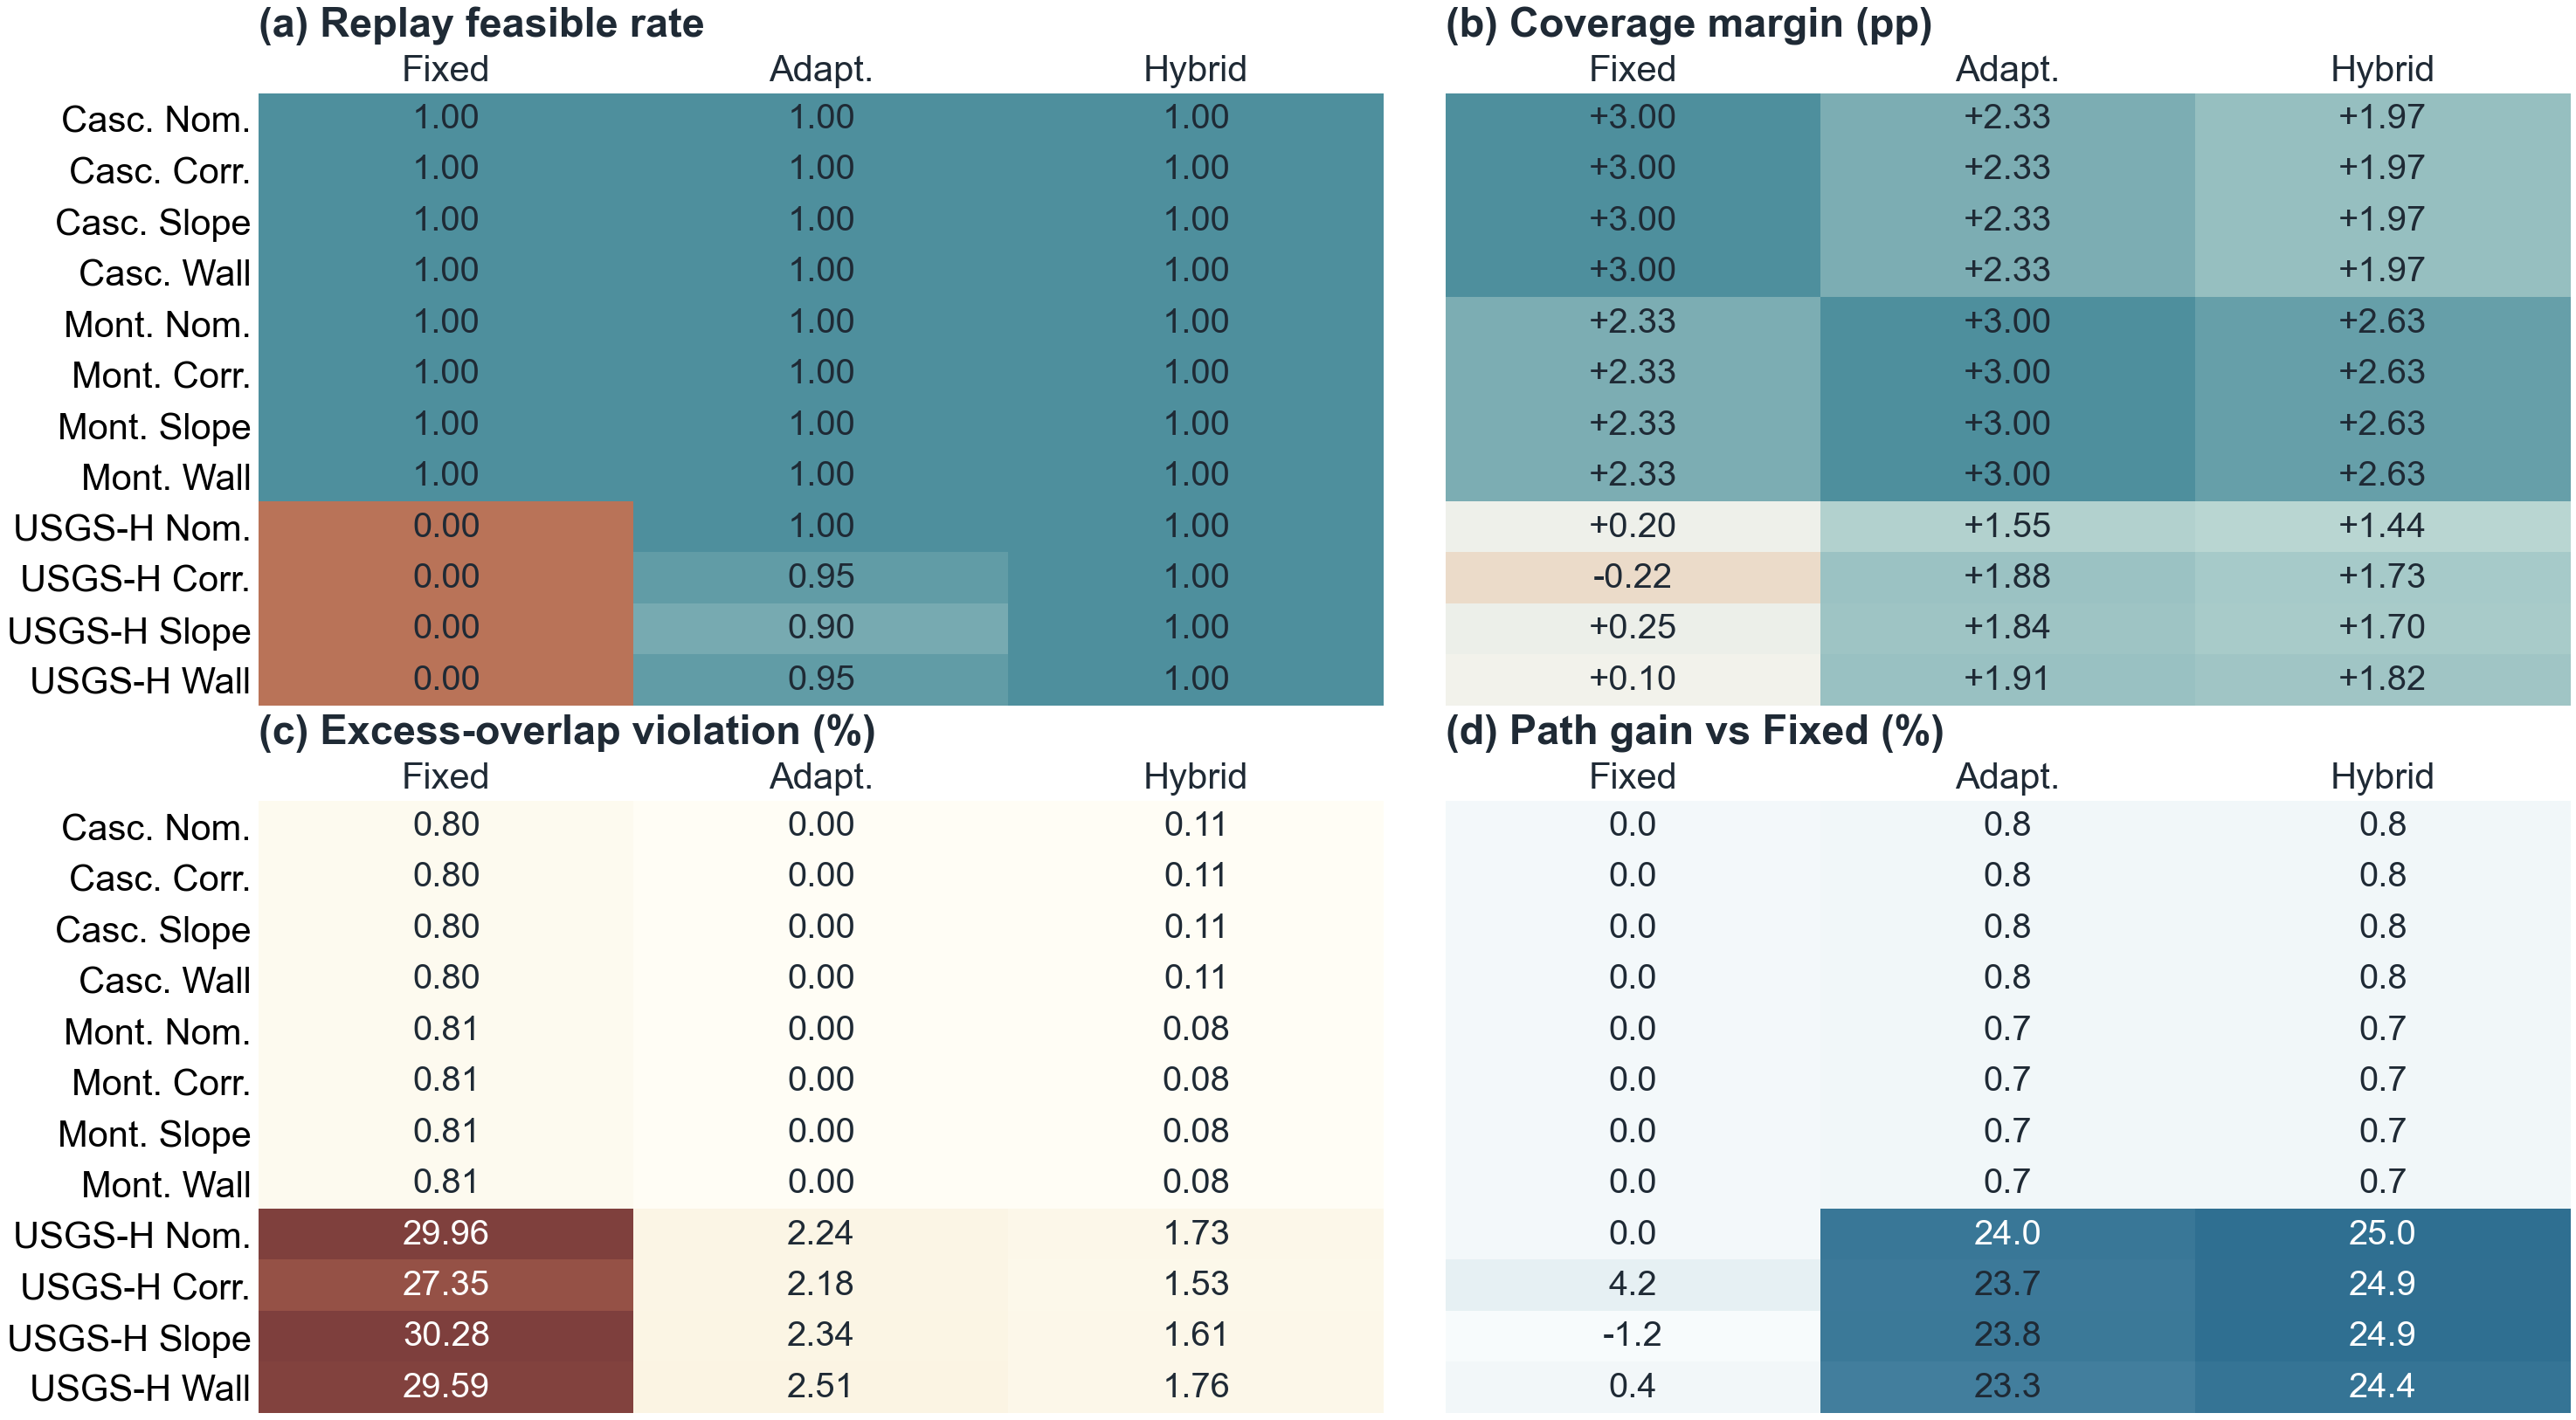
\includegraphics[width=\textwidth,height=0.36\textheight,keepaspectratio]{pic/journal_structured_prior_error_replay.png}
	\caption{Structured prior-error replay. The planner receives a perturbed prior bathymetry grid, while the final line family is replayed on the unperturbed truth grid. Rows combine scene and prior-error scenario; abbreviated row labels use Casc. for Cascadia, Mont. for Monterey, USGS-H for the high-complexity USGS crop, Nom. for nominal, Corr. for correlated bias, Slope for slope-amplified error, and Wall for localized wall bias. Columns compare Fixed-Spacing, Adaptive Spacing without GA, and Hybrid GA. The four panels report replay feasibility, replay coverage margin relative to the 97 percent acceptance gate, replay excess-overlap violation, and path gain relative to Fixed-Spacing. Color intensity and the printed cell values indicate feasibility loss, negative coverage margin, or overlap violation. The diagnostic is a controlled public-grid prior-error replay, not a calibrated geostatistical uncertainty model or a field survey.}
	\label{fig:structured_prior_error}
\end{figure}

The structured prior-error replay gives a controlled stress test between global bias checks and field validation. On the two GEBCO scenes, the selected line families and replay metrics are unchanged under the tested structured perturbations, so the primary public benchmark appears locally stable but is also not a demanding prior-error case. The USGS high-complexity crop is more informative. Fixed-Spacing remains infeasible in every structured-prior scenario, with mean replay excess-overlap violation near 27--30 percent. Adaptive Spacing remains much better than Fixed-Spacing but loses feasibility in some high-complexity prior-error runs, with replay feasibility of 0.90--0.95 under the non-nominal perturbations and excess overlap up to 2.51 percent. Hybrid GA remains feasible in all 20 seeds for all tested structured-prior scenarios, replaying at 98.70--98.82 percent coverage and 1.53--1.76 percent excess-overlap violation on the USGS high-complexity crop. Although this is still not field evidence, it supports treating GA refinement as optional local cleanup and a repeatability check in overlap-stressed terrain regimes.

\subsection{Execution-uncertainty Replay on Public Layouts}
Figure~\ref{fig:uncertainty_replay} reports the Monte Carlo execution-uncertainty replay defined in the protocol. The replay uses the selected public-scene layouts and injects global and correlated line drift, independent cross-track tracking error, heading error, local footprint-scale noise, and terrain-coupled footprint shrinkage after planning. It therefore tests coverage and overlap margin under perturbed execution assumptions without re-optimizing the line family.

\begin{figure}[!htbp]
	\centering
	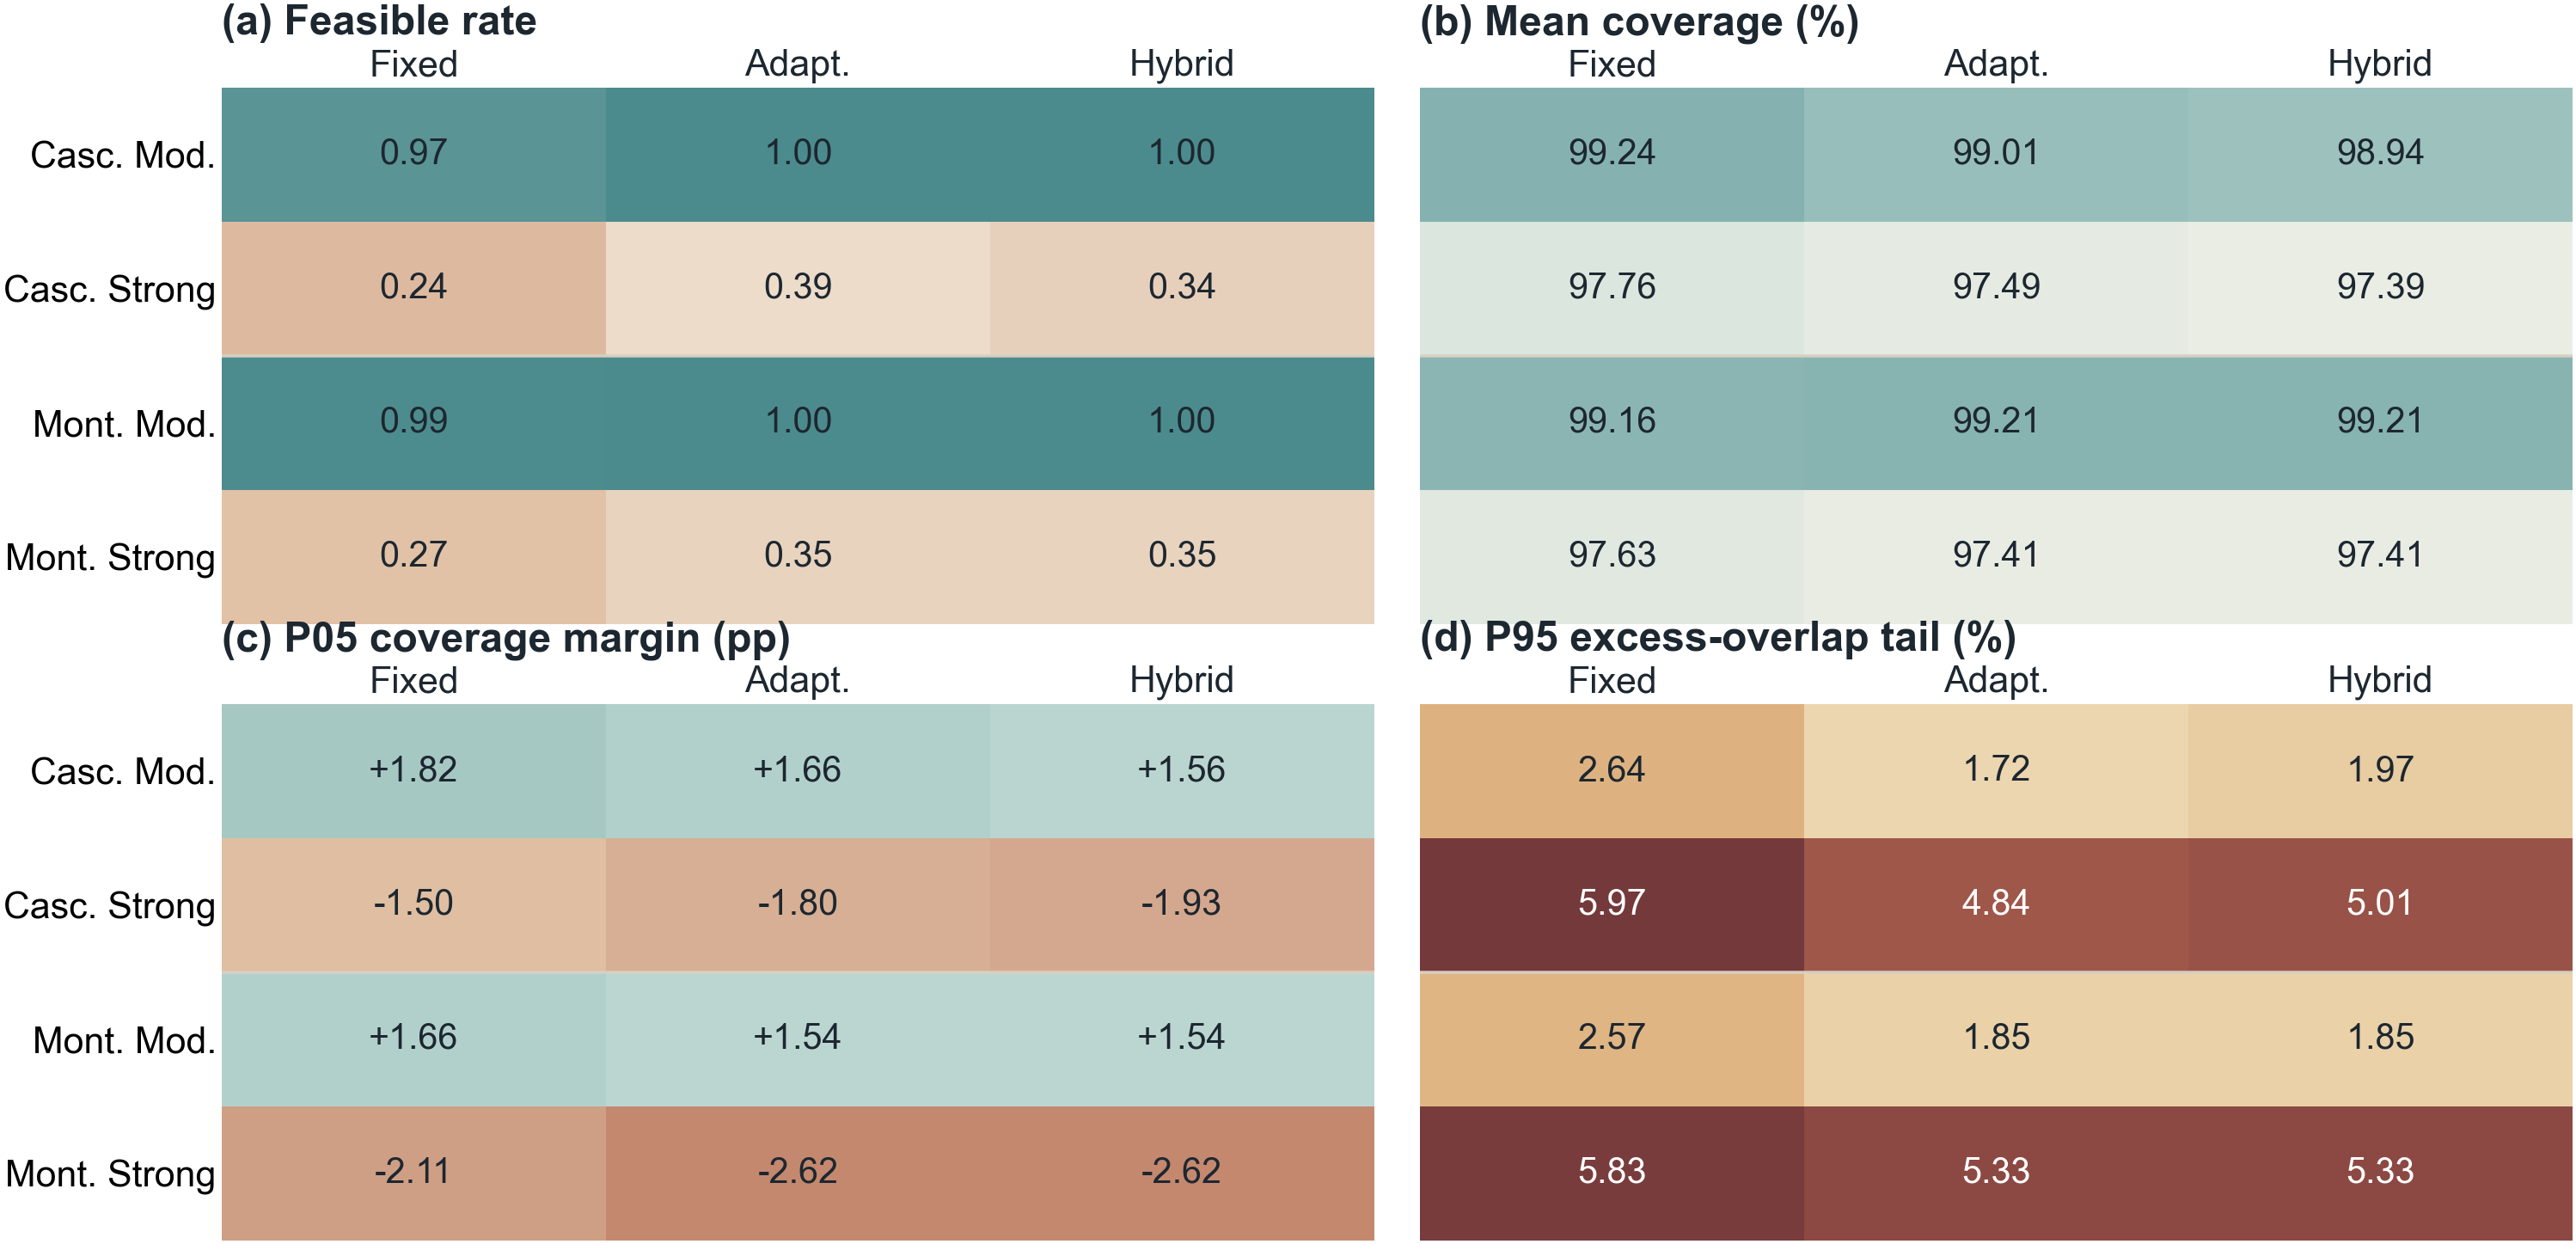
\includegraphics[width=\textwidth,height=0.33\textheight,keepaspectratio]{pic/journal_uncertainty_replay.png}
	\caption{Execution-uncertainty replay on the two public GEBCO layouts. Rows combine scene and perturbation level, with Mod. and Strong denoting the moderate and strong execution-error envelopes. Columns compare Fixed-Spacing, Adaptive Spacing without GA, and Hybrid GA. The four panels report feasibility rate, mean predicted coverage, fifth-percentile coverage margin relative to the 97 percent gate, and the 95th-percentile excess-overlap tail. Color intensity and the printed cell values indicate feasibility loss, negative lower-tail coverage margin, mean coverage below the gate, or overlap tail above the 3 percent gate. Under moderate perturbations, Hybrid GA remains feasible in 300/300 Cascadia trials and 299/300 Monterey trials; under strong perturbations, all methods lose substantial feasibility margin, indicating that execution-aware safety margins would be needed before field use.}
	\label{fig:uncertainty_replay}
\end{figure}

The moderate-noise replay keeps the public layouts mostly feasible even after adding correlated line drift and terrain-coupled footprint shrinkage. On Cascadia, the Hybrid GA layout averages 98.94 percent predicted coverage with 1.97 percent 95th-percentile excess overlap and a 1.000 feasibility rate, compared with 99.24 percent coverage, 2.64 percent 95th-percentile excess overlap, and a 0.967 feasibility rate for Fixed-Spacing. On Monterey, Hybrid GA averages 99.21 percent coverage with 1.85 percent 95th-percentile excess overlap and a 0.997 feasibility rate, compared with 99.16 percent coverage, 2.57 percent 95th-percentile excess overlap, and a 0.993 feasibility rate for Fixed-Spacing. The strong-noise setting is deliberately harsher: feasibility falls to roughly 0.24--0.39 across methods and scenes. The two regimes together indicate that geometry-aware layouts retain useful margin under moderate execution perturbations, while stronger correlated drift and footprint errors require explicit uncertainty-aware spacing margins and ultimately vehicle-level execution handling rather than the nominal planner alone.

\subsection{Uncertainty-aware Margin Replay}
The previous replay injects execution error after planning. To test whether the declared error envelope can be used prospectively, Figure~\ref{fig:uncertainty_margin_replay} adds an uncertainty-aware margin selector. The selector sweeps target-overlap margins from 5 to 30 percent and swath-profile quantiles from 0.18 to 0.34, generates a candidate terrain-aware line family, and accepts GA cleanup only when the nominal coverage and overlap gates are preserved. Candidate margins are ranked by replay performance under the same moderate and strong execution envelopes, and the selected layouts are then evaluated with 300 final Monte Carlo trials. This remains a pre-mission numerical selector rather than a closed-loop controller.

\begin{figure}[!htbp]
	\centering
	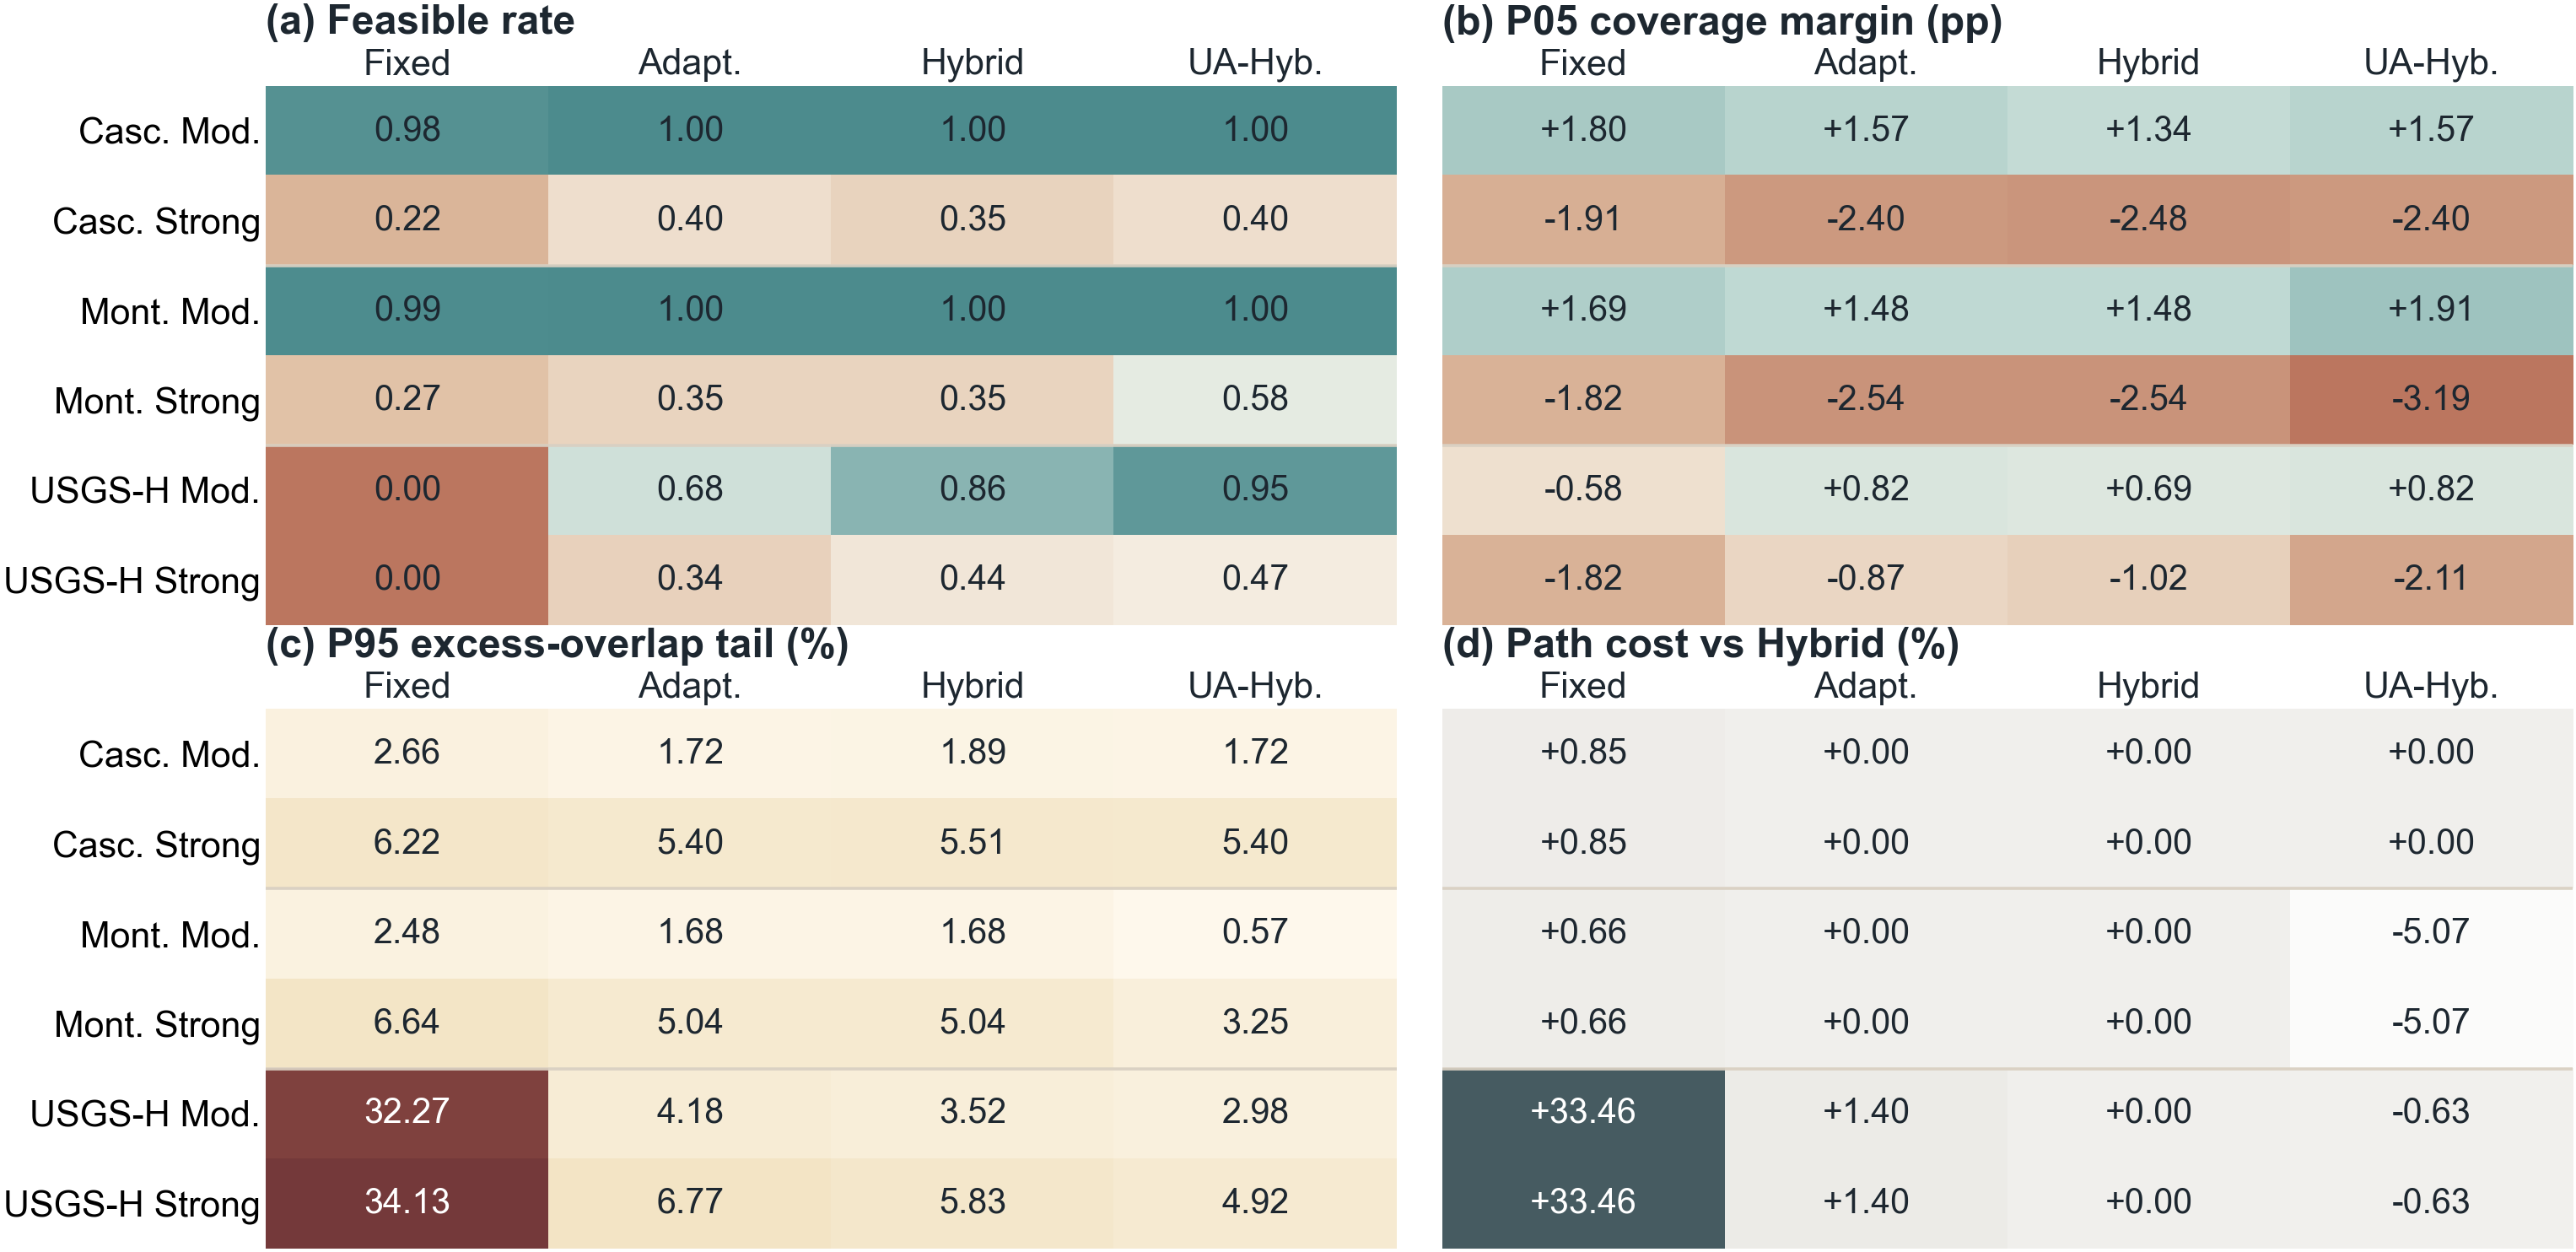
\includegraphics[width=\textwidth,height=0.33\textheight,keepaspectratio]{pic/journal_uncertainty_margin_replay.png}
	\caption{Uncertainty-aware margin selection under the declared execution-error envelope. Rows combine scene and perturbation level, with Mod. and Strong denoting the moderate and strong execution-error envelopes and USGS-H denoting the high-complexity USGS crop. Columns compare Fixed-Spacing, Adaptive Spacing without GA, Hybrid GA, and the selected uncertainty-aware margin variant (UA-Hybrid). The four panels report feasibility rate, fifth-percentile coverage margin relative to the 97 percent gate, 95th-percentile excess-overlap tail, and path-cost change relative to the nominal Hybrid GA. Color intensity and the printed cell values indicate feasibility loss, negative coverage margin, excess-overlap tail above the 3 percent gate, or path cost above 2 percent. The diagnostic selects a pre-mission spacing margin; it does not model current, control, SLAM feedback, or field logs.}
	\label{fig:uncertainty_margin_replay}
\end{figure}

The margin replay gives a mixed boundary. On Cascadia, the selected margin is essentially the nominal 15 percent overlap family, so UA-Hybrid changes little: under strong noise, feasibility rises only from 0.350 to 0.400 and the 95th-percentile excess-overlap tail decreases from 5.51 to 5.40 percent. Monterey shows a clearer selection effect. The selector chooses a 10 percent target-overlap, 0.18-quantile, \(75^{\circ}\) family with 72 lines; under moderate noise it keeps feasibility at 0.997 and reduces the 95th-percentile excess-overlap tail from 1.68 to 0.57 percent, while under strong noise feasibility rises from 0.353 to 0.580 and the overlap tail drops from 5.04 to 3.25 percent. However, the strong-noise fifth-percentile coverage margin remains negative, so the improvement is not a field-readiness guarantee. The USGS high-complexity crop is the most informative operational stress case: the selected 10 percent, 0.34-quantile margin raises moderate-noise feasibility from 0.863 to 0.953 and reduces the 95th-percentile excess-overlap tail from 3.52 to 2.98 percent, while preserving a small path reduction relative to the nominal Hybrid layout. Under strong noise, the USGS overlap tail also improves from 5.83 to 4.92 percent, but feasibility remains below 0.5. Declared uncertainty margins can improve moderate execution-transfer robustness and expose safer design choices, but strong correlated drift still requires vehicle/controller-level treatment.

\subsection{Current-drift Execution Replay}
The previous uncertainty replay treats execution error as a declared statistical envelope. A more operation-facing current-drift replay converts mild, cross, and adverse current proxies into residual cross-track line drift, heading perturbation, low-frequency footprint variation, and terrain-coupled footprint shrinkage before recomputing the same public-grid coverage and overlap metrics. The proxy uses current speeds of 0.05, 0.15, and 0.30~m~s\(^{-1}\), respectively, and reports the resulting 95th-percentile residual drift as a fraction of local line spacing. It is not a hydrodynamic simulator or sea trial; it is a first-order stress replay designed to show whether the line geometry has usable margin when current-induced tracking error is introduced after planning. The full current-drift heatmap is retained in the reproducibility package rather than promoted as another main-text figure, because the key evidence is the bounded numerical outcome reported below.

The current-drift replay is intentionally bounded rather than uniformly positive. Under mild and cross-current proxies, the terrain-aware layouts remain feasible on the two GEBCO scenes and on the USGS high-complexity crop, while Fixed-Spacing remains infeasible on the USGS crop because its nominal overlap violation is already too large. Under the adverse-current proxy, Cascadia remains mostly feasible: Hybrid GA reaches a 0.980 feasibility rate, a positive 0.51 percentage-point fifth-percentile coverage margin, and a 1.87 percent 95th-percentile excess-overlap tail; UA-Hybrid slightly improves these to 0.983, 0.63 percentage points, and 1.72 percent, respectively. Monterey is the clearer margin-selection case. The nominal Hybrid layout falls to 0.903 feasibility with a negative fifth-percentile coverage margin of \(-0.55\) percentage points, whereas UA-Hybrid reaches 0.963 feasibility, restores the fifth-percentile coverage margin to \(+0.37\) percentage points, and lowers the 95th-percentile excess-overlap tail from 1.80 to 0.91 percent. On the USGS high-complexity crop, UA-Hybrid does not improve adverse-current feasibility relative to nominal Hybrid (0.860 versus 0.863) and its fifth-percentile coverage margin remains negative at \(-0.68\) percentage points, although the overlap tail is lowered from 3.66 to 2.98 percent. Margin-aware spacing can help under a declared current-drift proxy, especially on Monterey, but stronger current and controller effects still need to be modeled inside an execution-aware planner rather than treated as a post-hoc replay.

\subsection{Independent USGS 30 m Public-grid Extension}
To check whether the overlap-control pattern is only an artifact of the two regional GEBCO windows, we ran a separate extension on a higher-resolution public GeoTIFF from the USGS Southern Cascadia composite multibeam bathymetry release \cite{dartnell2026southerncascadia}. This extension is not mixed into the primary benchmark. It uses three automatically selected \(4 \times 5\) nautical-mile crops from the USGS grid at low, medium, and high empirical terrain-complexity quantiles, and it repeats the same Fixed-Spacing, Adaptive Spacing without GA, and Hybrid GA comparison with 50 Hybrid GA seeds.

	\begin{figure}[!htbp]
		\centering
		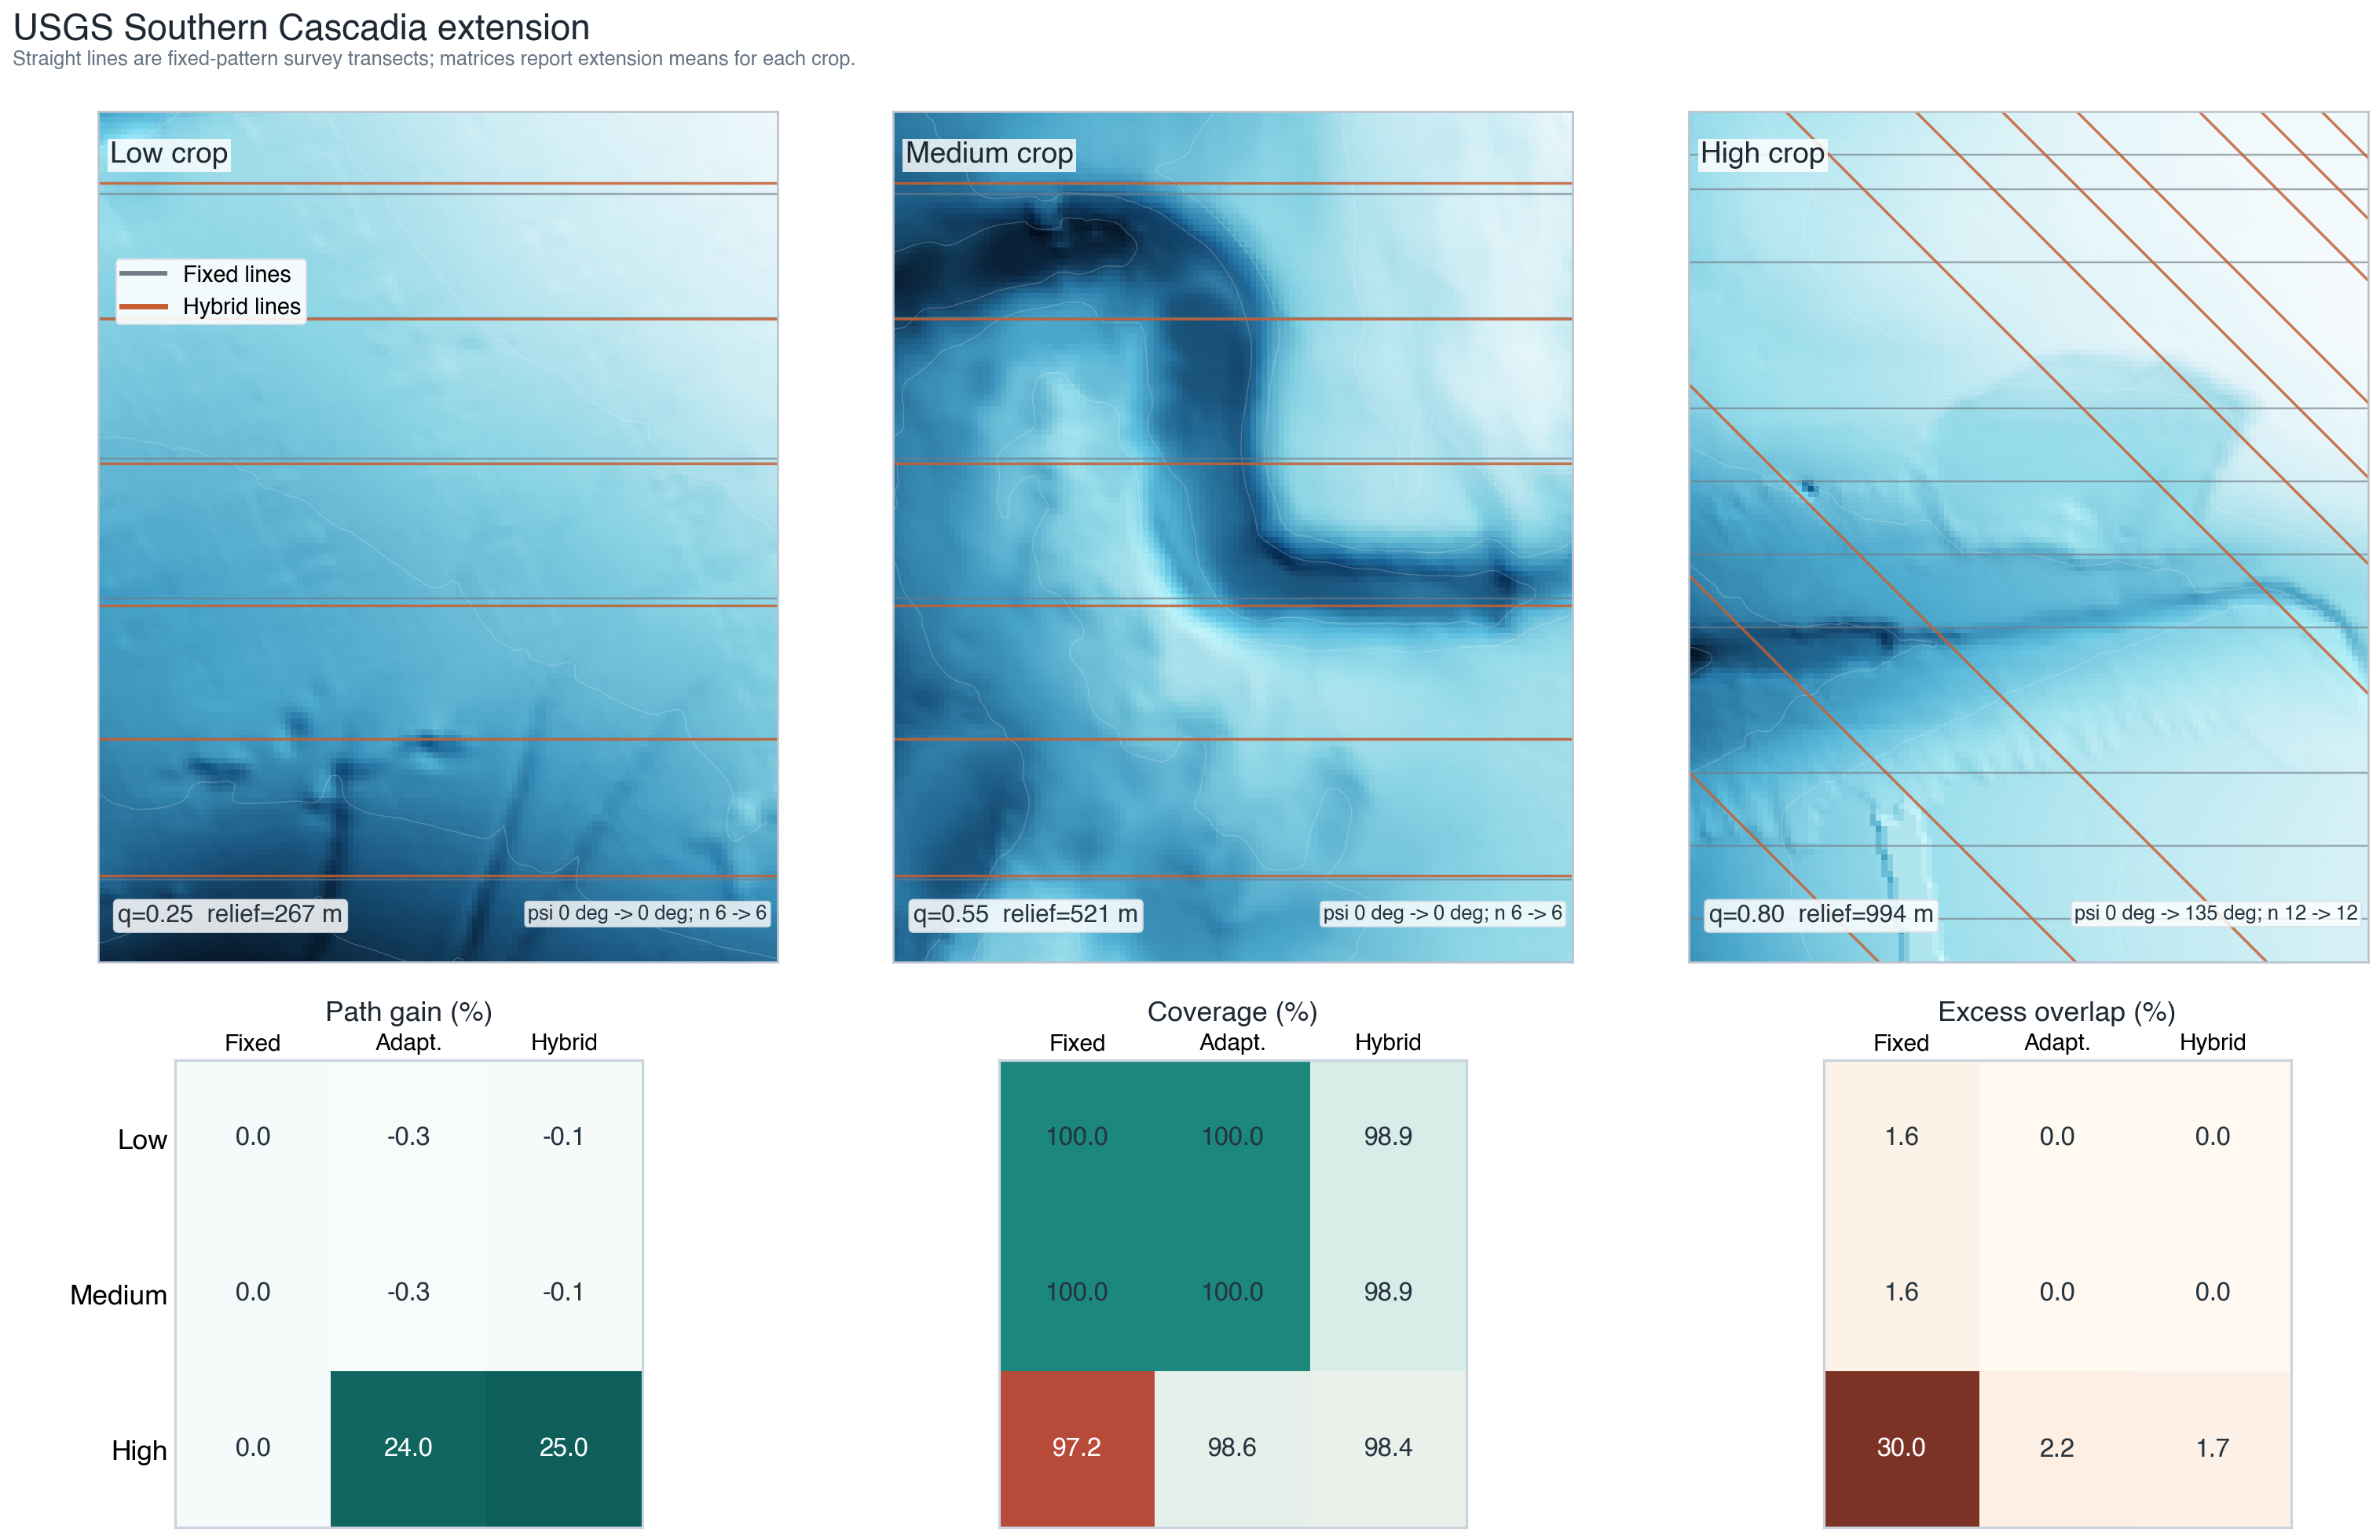
\includegraphics[width=\textwidth,height=0.50\textheight,keepaspectratio]{pic/journal_usgs_extension.png}
		\caption{Independent USGS Southern Cascadia 30~m multibeam-derived public-grid extension. The top row shows the three selected crops with Fixed-Spacing and representative Hybrid GA line families, ordered by empirical terrain complexity from low to high and drawn without map-axis distortion. The bottom row reports benchmark means for path gain relative to Fixed-Spacing, predicted coverage, and excess-overlap violation recomputed from the extension CSV/JSON outputs. These plotted straight transects are planned fixed-pattern survey-line families, not free-form vehicle trajectories. The extension remains a public-grid numerical check, not an additional sea-trial or mission-log validation.}
		\label{fig:usgs_extension}
	\end{figure}

The extension supports a more specific interpretation of the contribution. On the low- and medium-complexity USGS crops, Fixed-Spacing was already feasible with 100.00 percent predicted coverage and 1.633 percent excess overlap, so terrain-aware planning mainly removed the small overlap surplus at a negligible path-length cost. On the high-complexity crop, however, Fixed-Spacing produced 29.960 percent excess overlap and was infeasible under the reported acceptance rule. Adaptive Spacing without GA shortened the path by 24.02 percent, reached 98.55 percent predicted coverage, and lowered excess overlap to 2.237 percent. The 50-seed hybrid layout reached 98.42 percent predicted coverage, 1.752 percent excess overlap, and a 25.07 percent path gain. The extension therefore reinforces the same mechanism under a stricter public-grid setting: terrain-aware spacing matters most when the terrain genuinely stresses the fixed-spacing assumption, whereas easier public-grid crops should not be expected to show large route savings.

\subsection{Threshold and Local-failure Diagnostics}
The default 97 percent coverage and 3 percent mean-excess-overlap gate is useful for method comparison, but it is not a hydrographic acceptance rule. To test whether the reported means hide stricter-threshold or local-tail failures, we added a threshold and local-failure diagnostic on the two primary GEBCO scenes and on the USGS high-complexity crop. Fixed-Spacing and Adaptive Spacing without GA are deterministic in this diagnostic; Hybrid GA is reported over 20 seeds. The diagnostic records pass rates for coverage thresholds of 95, 97, 98, 99, and 99.5 percent crossed with mean-excess-overlap gates of 1, 2, 3, and 5 percent, and it also reports the largest connected uncovered patch and cellwise excess-overlap tails.

\begin{figure}[!htbp]
	\centering
	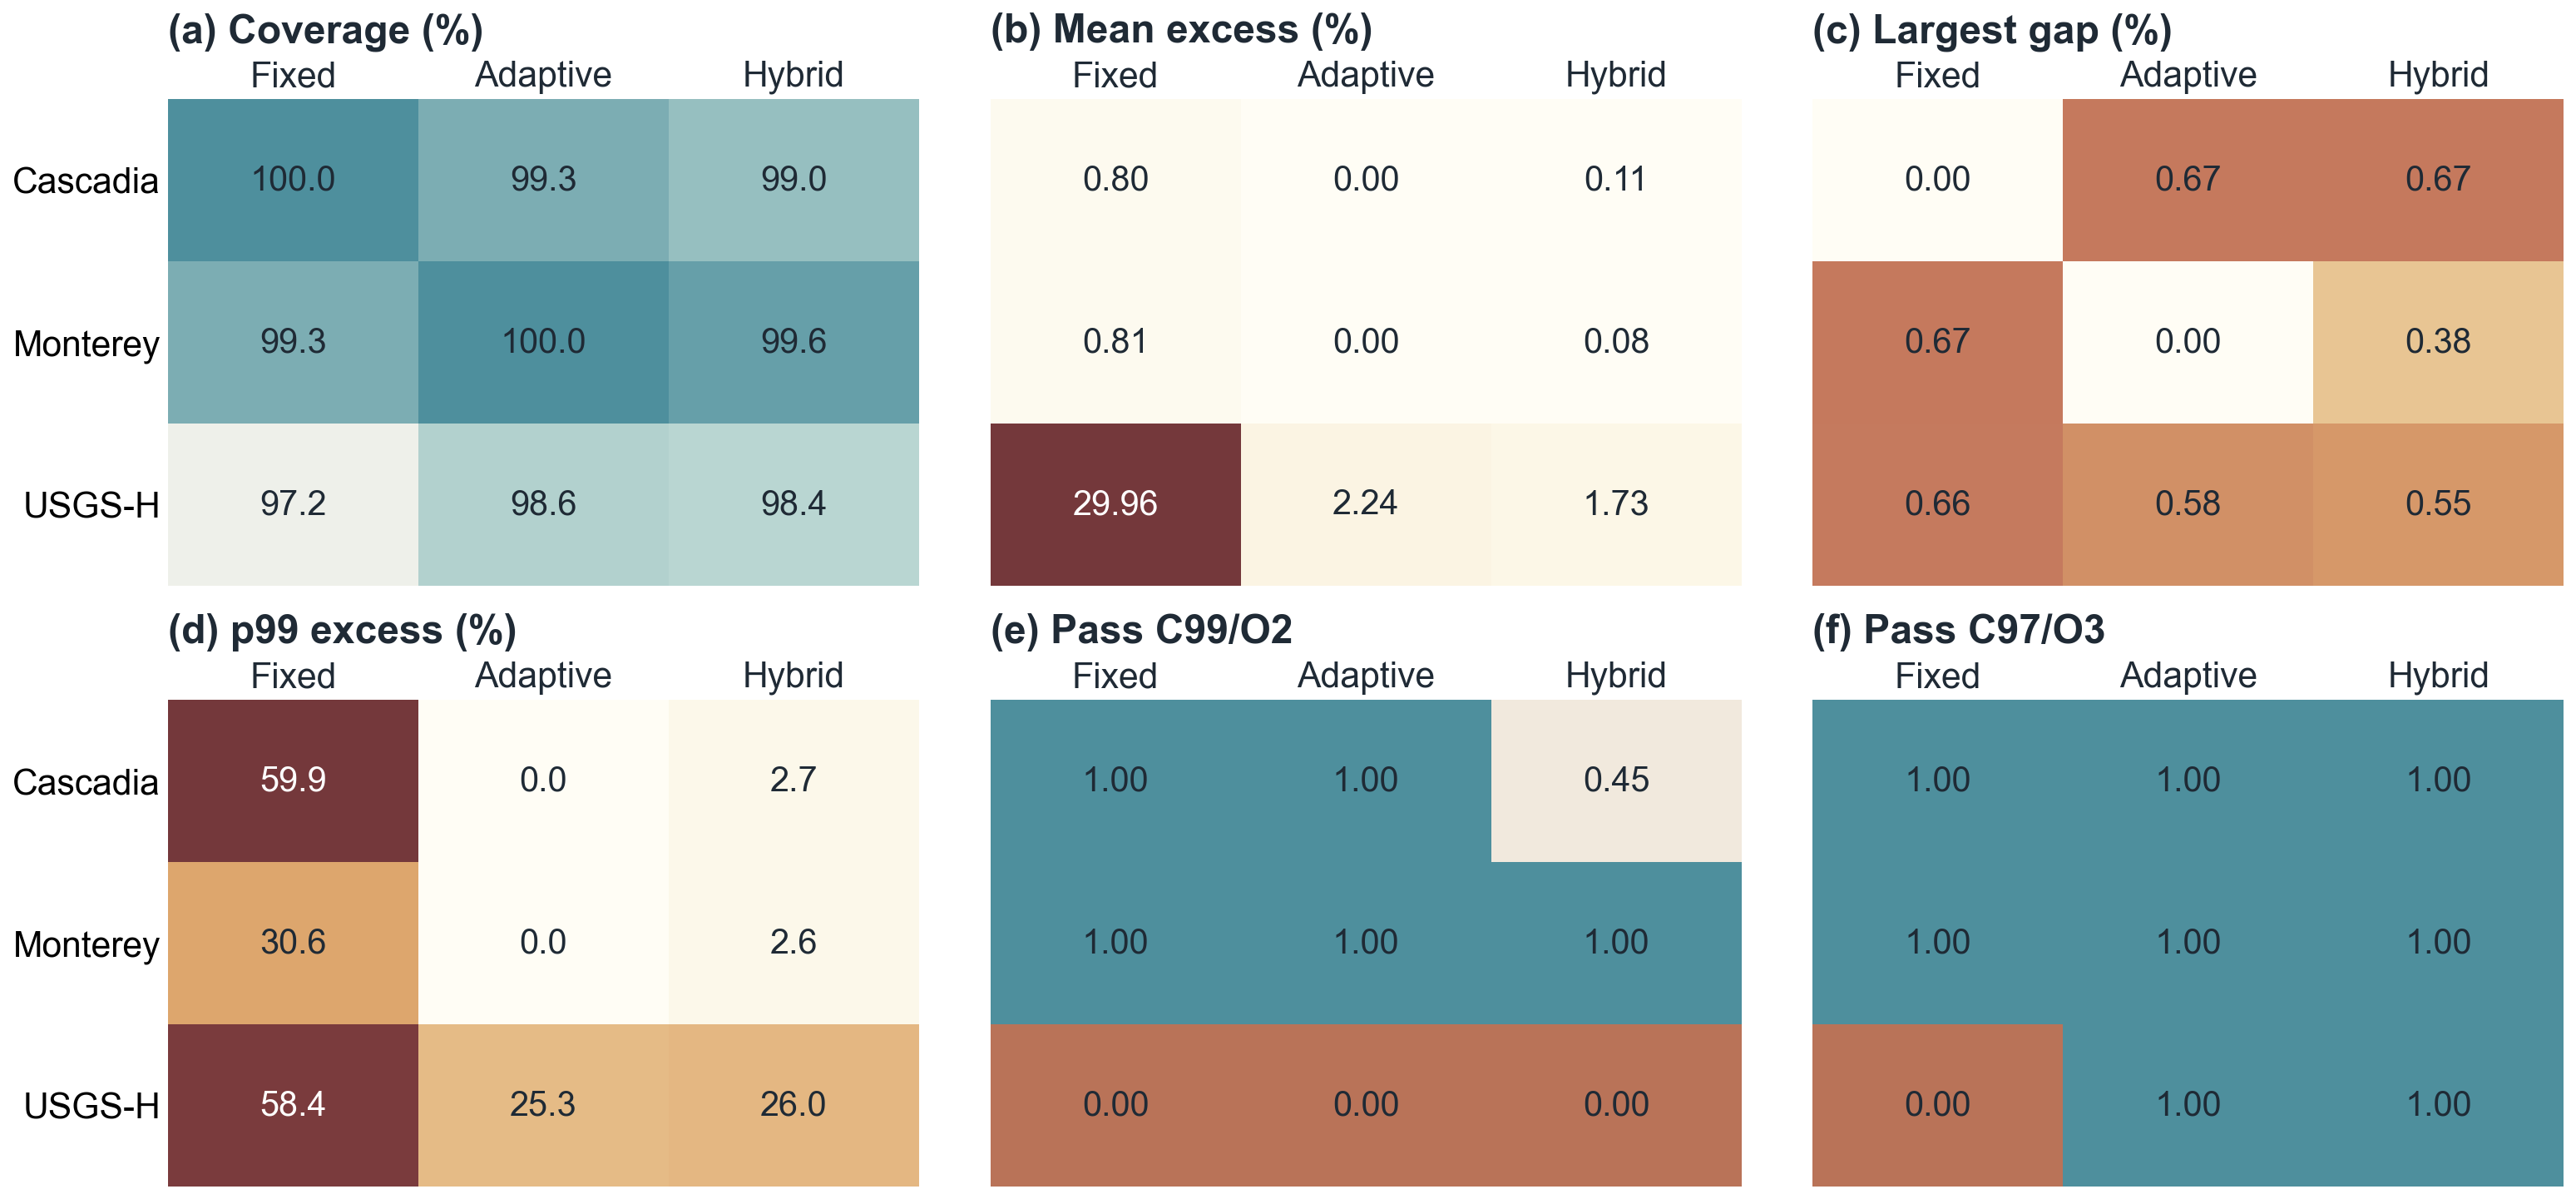
\includegraphics[width=\textwidth]{pic/journal_threshold_local_failure.png}
	\caption{Threshold and local-failure diagnostic for the two primary GEBCO scenes and the USGS high-complexity crop. The figure reports mean coverage, mean excess-overlap violation, largest connected uncovered patch, the 99th-percentile cellwise excess-overlap tail, and pass rates under both the stricter \(C99/O2\) screen and the manuscript's default \(C97/O3\) benchmark gate. Hybrid GA values are 20-seed means; Fixed-Spacing and Adaptive Spacing without GA are deterministic. The diagnostic is a raster-evaluator audit designed to expose local failures hidden by scene-level means; it is not hydrographic QA or a field-survey acceptance test.}
	\label{fig:threshold_local_failure}
\end{figure}

Figure~\ref{fig:threshold_local_failure} sharpens the interpretation of the public results. Under the manuscript's default \(C97/O3\) gate, the Hybrid GA remains feasible on all three audited scenes, while Fixed-Spacing remains infeasible on the USGS high-complexity crop because its mean excess overlap is 29.960 percent. Under the stricter \(C99/O2\) screen, however, the conclusion becomes more cautious: Hybrid GA passes all Monterey seeds but only 45 percent of Cascadia seeds and no USGS high-complexity seeds. Adaptive Spacing without GA passes the stricter screen on the two GEBCO scenes but not on the USGS high-complexity crop, where mean coverage is 98.55 percent and mean excess overlap is 2.237 percent.

The local-tail metrics explain why this distinction matters. On the GEBCO pair, Fixed-Spacing can satisfy the strict mean screen while still producing large localized p99 cellwise excess-overlap values of 59.89 percent on Cascadia and 30.56 percent on Monterey, because the high-overlap cells occupy only a small fraction of the domain. On the USGS high-complexity crop, the reported hybrid layout lowers the mean excess-overlap violation from 29.960 to 1.732 percent and lowers the nonzero-excess-overlap cell share from 90.66 to 24.27 percent, but the p99 cellwise tail remains high at 26.03 percent. This negative boundary strengthens the claim discipline: terrain-aware spacing is sufficient to make the USGS high-complexity crop feasible under the declared benchmark gate, but pointwise or tail-constrained overlap control would be needed before claiming project-specific survey quality.

\subsection{Side-specific Footprint Validity Audit}
The main evaluator uses a total-width proxy for raster coverage and adjacent-spacing overlap. To test whether this simplification changes the benchmark interpretation, we added a side-specific footprint audit on the two primary GEBCO scenes and the USGS high-complexity crop. For each scene, the audit reconstructs the Fixed-Spacing, Adaptive Spacing without GA, and seed-0 Hybrid layouts, recomputes port and starboard cross-track reach separately under the same local planar model and clipping limits, and compares the resulting raster counts against the total-width proxy. This diagnostic is not beam-level acoustic ray tracing; it is a planning-evaluator validity check that asks whether preserving port/starboard asymmetry would overturn the headline feasibility conclusion.

\begin{figure}[!htbp]
	\centering
	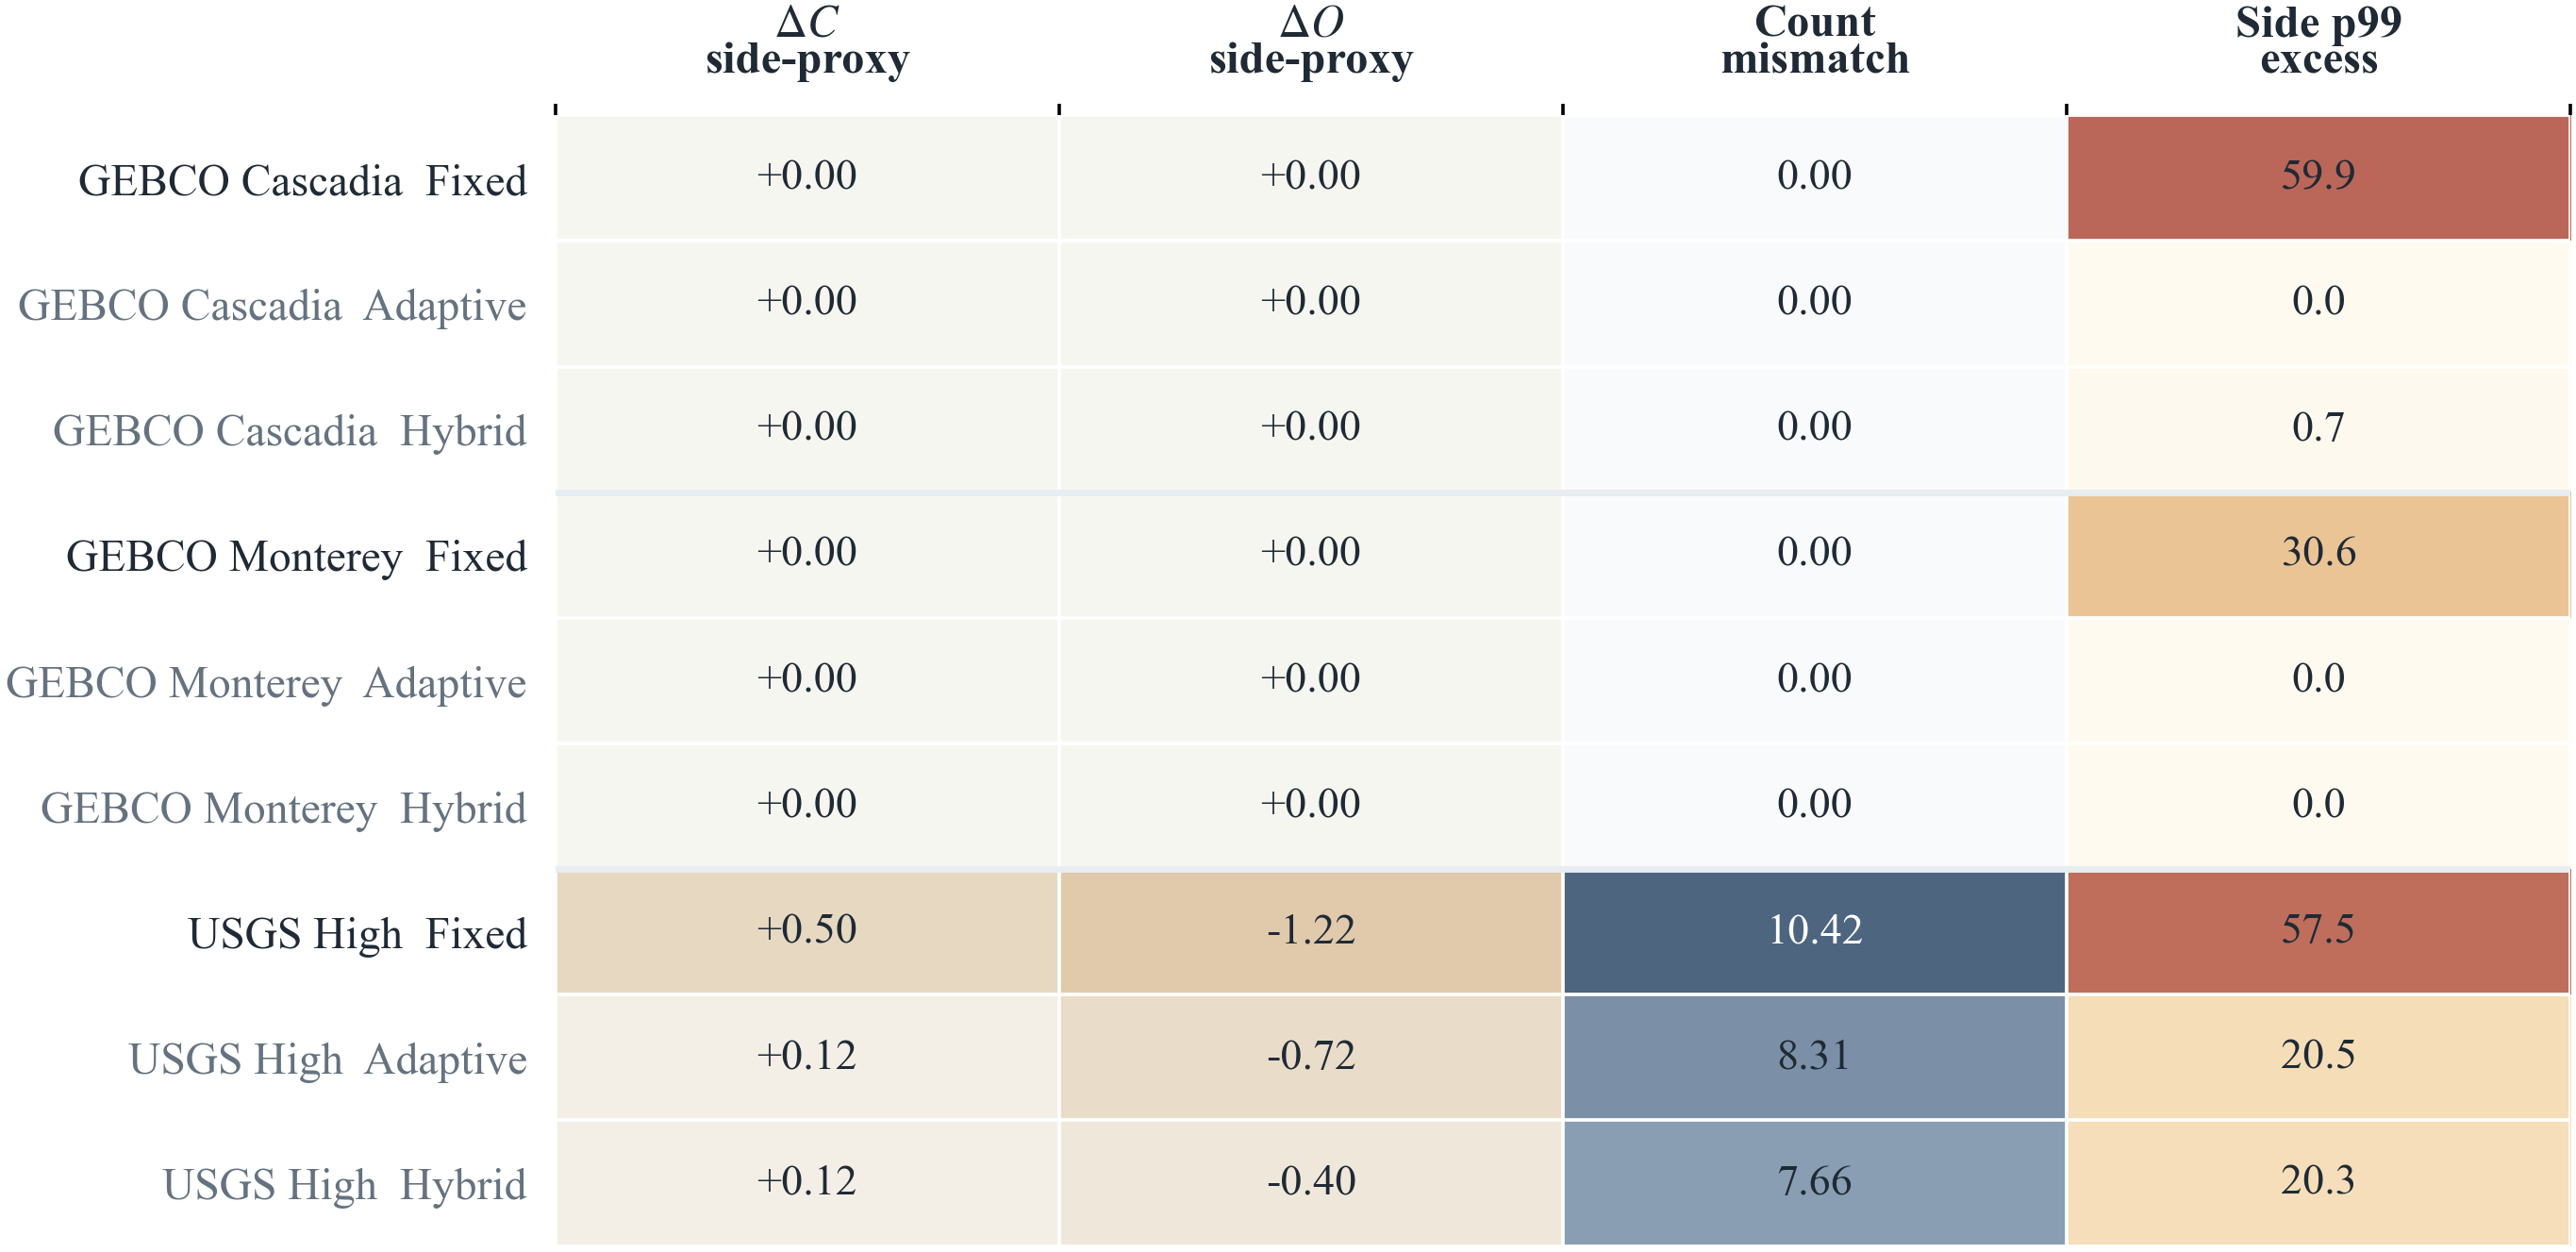
\includegraphics[width=\textwidth,height=0.44\textheight,keepaspectratio]{pic/journal_footprint_validity_audit.png}
	\caption{Side-specific footprint validity audit for representative layouts on the two GEBCO public scenes and the USGS high-complexity crop. The audit preserves port/starboard reach asymmetry and compares the resulting raster counts with the manuscript total-width proxy. \(\Delta C\) and \(\Delta O\) denote side-specific minus proxy coverage and mean excess-overlap differences; cell-count disagreement reports the fraction of grid cells whose coverage multiplicity changes; side p99 excess reports the side-specific 99th-percentile cellwise excess-overlap tail. The audit checks evaluator stability for planning conclusions; it is not beam-level acoustic ray tracing, raw MBES product validation, or hydrographic QA.}
	\label{fig:footprint_validity_audit}
\end{figure}

Figure~\ref{fig:footprint_validity_audit} shows that the side-specific audit does not change any audited \(C97/O3\) feasibility decision. Across the nine representative scene--method layouts, the maximum absolute coverage difference is 0.50 percentage points and the mean absolute difference is 0.083 percentage points. The corresponding maximum and mean absolute differences in mean excess-overlap violation are 1.217 and 0.260 percentage points, respectively. The largest differences occur on the USGS high-complexity crop, where the total-width proxy and side-specific counts disagree locally in 10.42 percent of cells for Fixed-Spacing, 8.31 percent for Adaptive Spacing without GA, and 7.66 percent for the representative Hybrid layout. Even there, the feasibility interpretation is stable: Fixed-Spacing remains infeasible, while Adaptive Spacing and the representative Hybrid layout remain feasible under the declared \(C97/O3\) gate. The audit therefore supports the benchmark-level conclusion while also showing why the evaluator should not be described as survey-product QA.

\subsection{Coarse-prior to Fine-grid Public Replay}
The preceding diagnostics still plan and evaluate on nominally matched grids, so we add a stricter public-grid replay on the same USGS source. Three USGS crops are selected by the same low/medium/high terrain-complexity policy, but the planner is given only coarsened prior surfaces with target cells of 120, 300, 600, and 900~m. The resulting line family is then replayed on a finer \(300 \times 240\) public grid with an effective cell size of about 31.0~m, without re-optimizing the heading or cross-track positions. This experiment is still a numerical public-data replay rather than a mission-log validation, but it tests whether the line layout survives a meaningful prior-resolution mismatch.

\begin{figure}[!htbp]
	\centering
	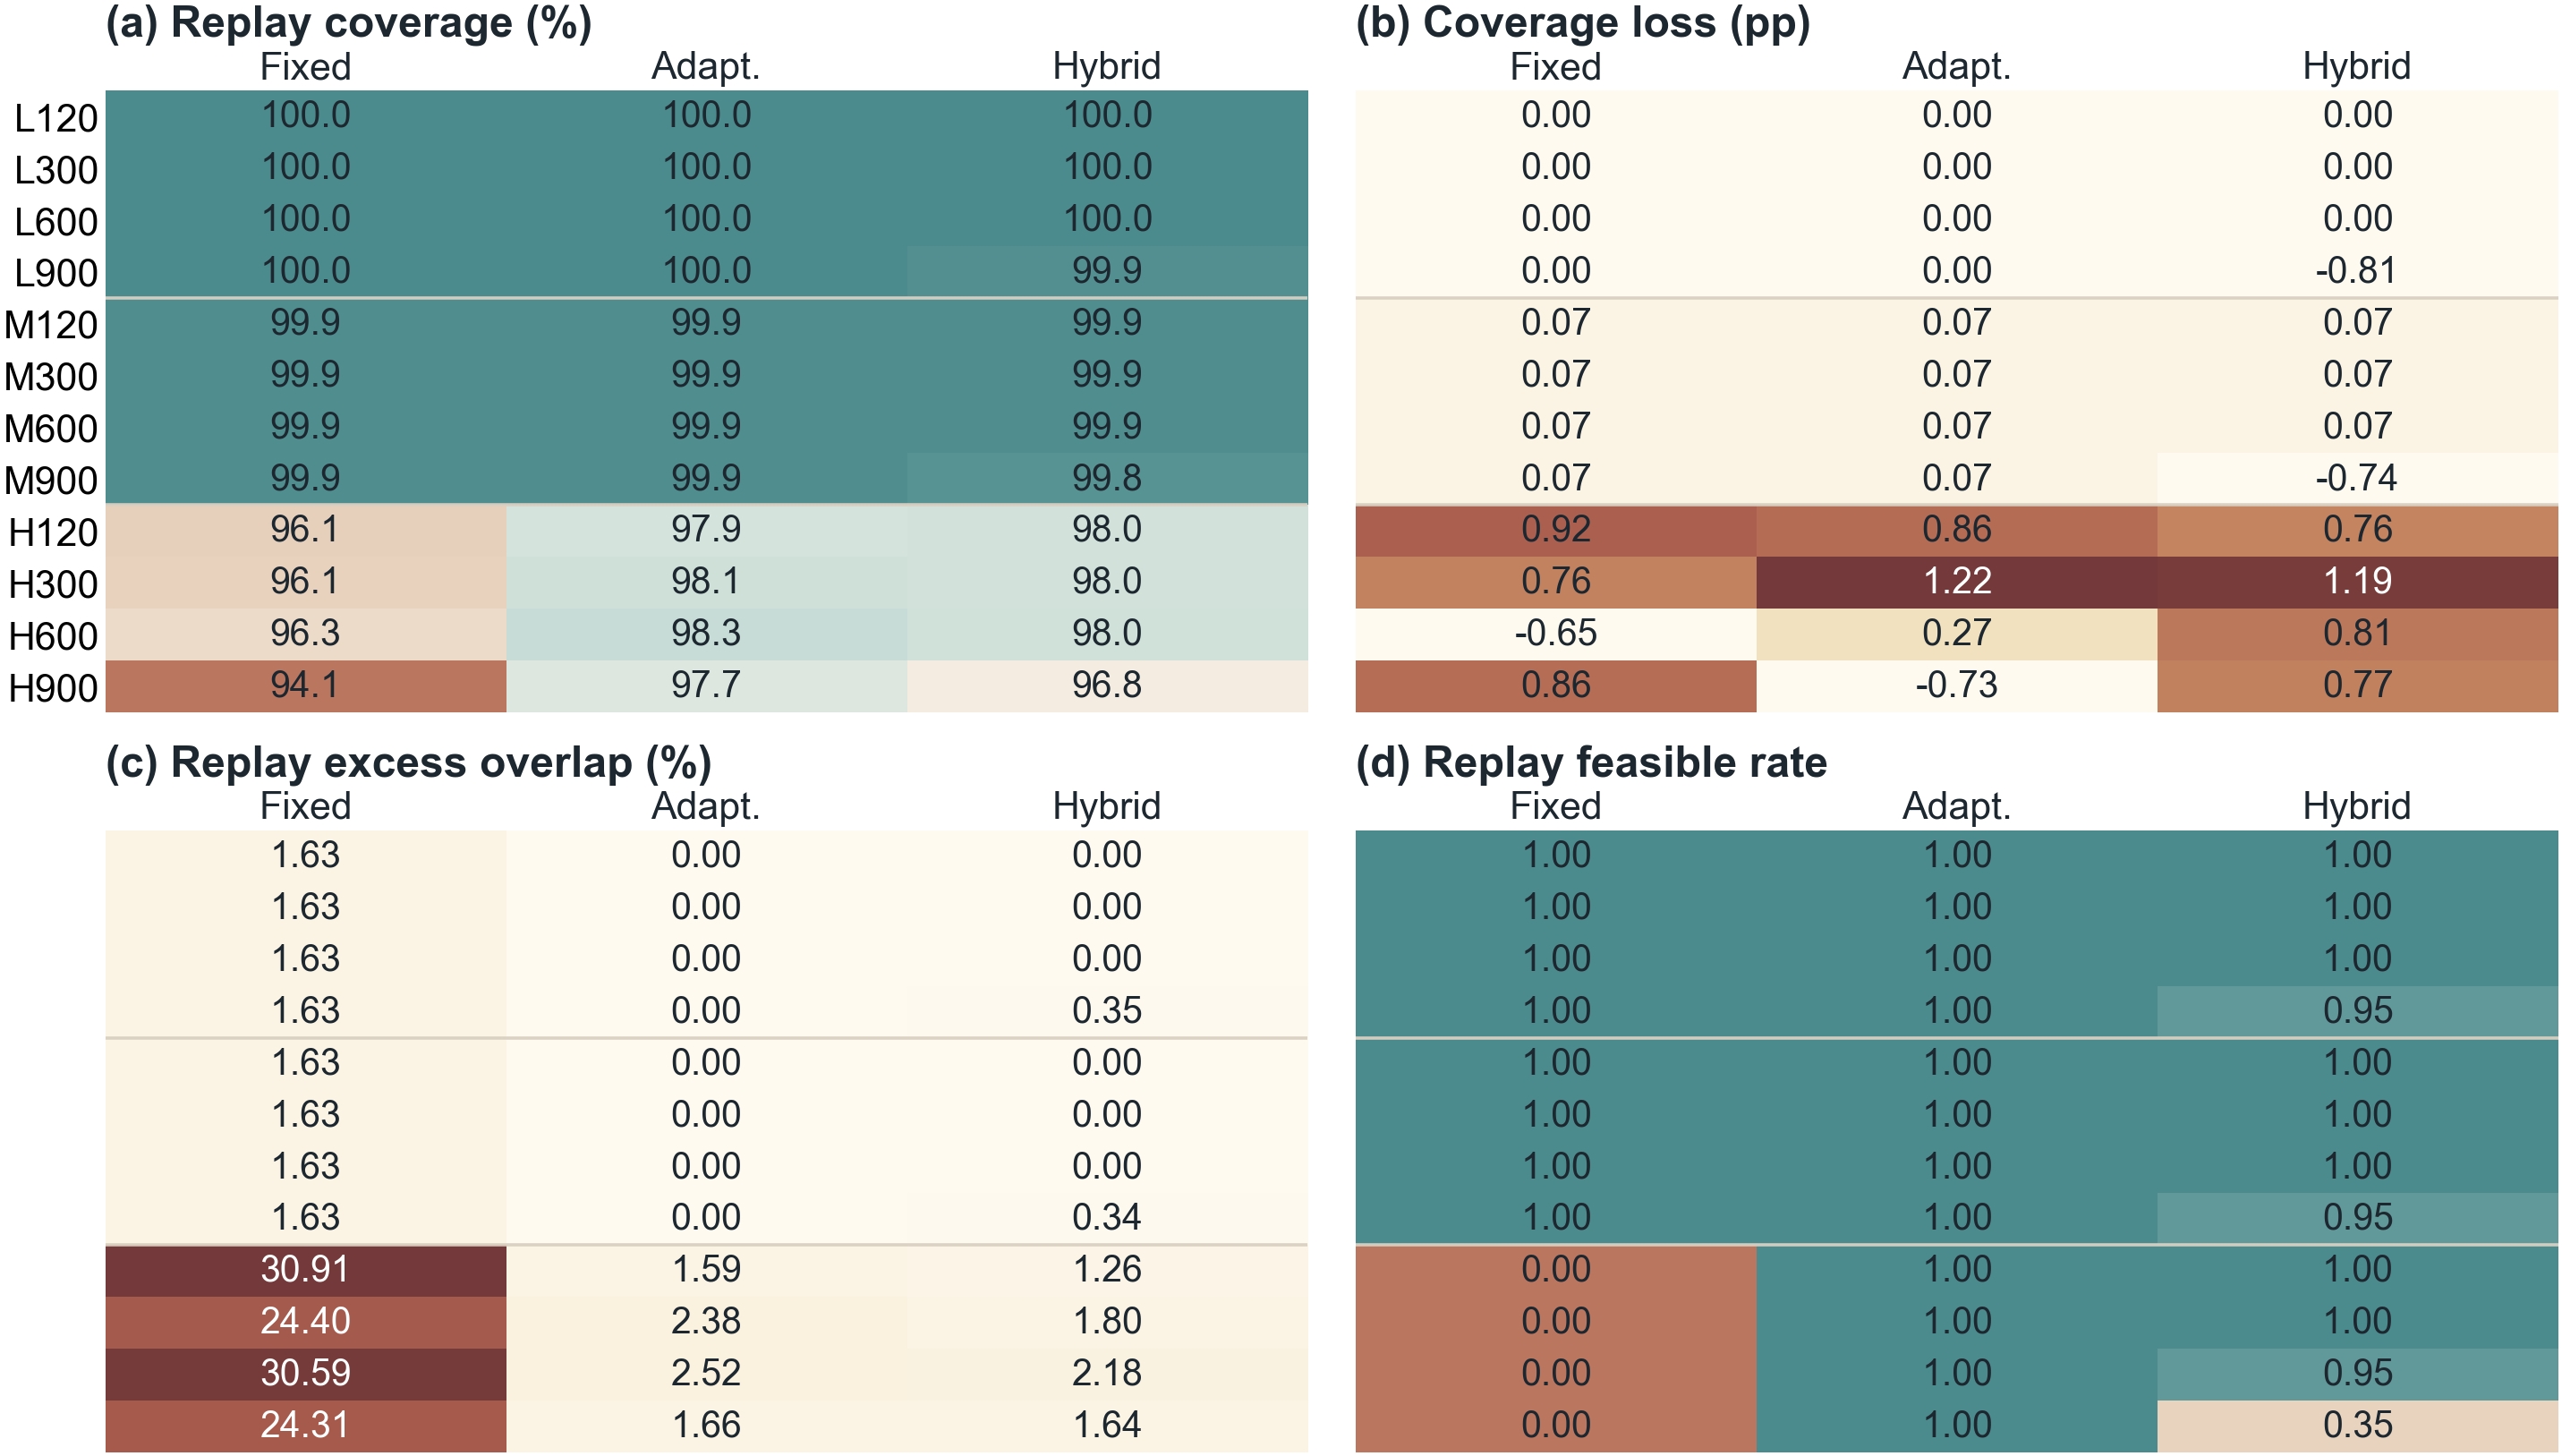
\includegraphics[width=\textwidth,height=0.36\textheight,keepaspectratio]{pic/journal_coarse_prior_replay.png}
	\caption{Coarse-prior to fine-grid replay on the USGS Southern Cascadia public bathymetry grid. Low, medium, and high-complexity crops are planned on 120, 300, 600, and 900~m coarsened priors, then the same fixed-pattern line families are replayed on the fine public grid without re-optimization. Row labels abbreviate crop complexity and prior cell size, e.g., L120, M300, and H900. The heatmaps report replay coverage, coverage loss relative to the coarse-prior prediction, replay excess-overlap violation, and replay feasibility. All entries are recomputed from \texttt{coarse\_prior\_replay/coarse\_prior\_replay\_summary.csv}; Hybrid GA values are 20-seed means for this diagnostic.}
	\label{fig:coarse_prior_replay}
\end{figure}

Figure~\ref{fig:coarse_prior_replay} shows that the easy and medium USGS crops remain insensitive to this prior coarsening: all methods replay at 99.93--100.00 percent coverage, but Fixed-Spacing keeps about 1.63 percent excess overlap whereas the terrain-aware layouts remove that surplus. The high-complexity crop is more informative. Fixed-Spacing remains infeasible after replay at all four prior resolutions, with 95.42--96.32 percent coverage and 24.36--30.91 percent excess overlap. Hybrid GA remains feasible or nearly feasible for the 120, 300, and 600~m priors, replaying at 97.99--98.03 percent coverage, limiting excess overlap to 1.26--2.18 percent, and giving 17.81--27.37 percent replay path gain relative to Fixed-Spacing. The 900~m prior is the negative boundary: Hybrid GA still limits excess overlap to 1.64 percent and gives a 16.45 percent replay path gain, but replay coverage drops to 96.81 percent and the replay feasibility rate falls to 0.35. The mechanism claim therefore remains bounded: terrain-aware spacing is stable under moderate controlled prior-resolution mismatch on the tested public grid, but very coarse priors can erase the coverage margin.

\subsection{Supplementary and Reproducibility Evidence}
The main text keeps the figures that change the interpretation of the method, while secondary diagnostics are supplied as reproducibility artifacts. The equal-budget PSO comparison, external heuristic layout audit, external turning-cost audit, GA surrogate-audit heatmap, full target-overlap matrix, grid-resolution matrix, prior-depth and relief-scale checks, penalty-weight grid, submission-boundary \(W_{\max}\)/GA-gate CSV and JSON files, threshold/local-failure CSV and JSON files, side-specific footprint validity CSV/JSON/PNG files, and full current-drift replay heatmap are retained as generated artifacts. Their role is auditability: they allow a reviewer to trace optimizer dependence, external baseline dependence, turn-radius cost dependence, surrogate-evaluator agreement, declared-parameter sensitivity, prior-map robustness, evaluator simplification, local-tail behavior, and execution-boundary claims without turning the Results section into a figure appendix. For the same reason, the current-drift heatmap is not promoted as a visual headline; the manuscript reports the bounded numerical outcome and treats the heatmap as supporting evidence.

To make the formula-to-code relationship auditable, Table~\ref{tab:implementation_map} maps the main mathematical objects to the implementation files and output artifacts used in this submission. The table is intentionally compact: it does not replace the public repository, but it lets a reviewer trace every headline quantity from the manuscript to a script or CSV/JSON file.

\begin{table}[!htbp]
	\centering
	\caption{Implementation map linking the manuscript notation to reproducible scripts and output files. The table identifies where the main sensor--terrain model, planner variants, diagnostic gates, and reported public-window statistics are generated.}
	\label{tab:implementation_map}
	\tiny
	\renewcommand{\arraystretch}{1.10}
	\setlength{\tabcolsep}{2.0pt}
	\begin{tabular}{@{}p{0.24\linewidth}p{0.32\linewidth}p{0.34\linewidth}@{}}
		\toprule[1bp]
		\textbf{Manuscript quantity} & \textbf{Implementation location} & \textbf{Primary output artifacts} \\
		\midrule[1bp]
		Swath model \(W(x)\), coverage \(CR\), overlap \(O_{\mathrm{ex}}\) & Core evaluator script & \texttt{run\_5/} benchmark results, method statistics, and public figures \\
		Fixed, Greedy, Adaptive, Hybrid variants & Core script plus \texttt{run\_5/} settings record & \texttt{run\_5/} summary and implementation details \\
		Nine-window paired statistics & \texttt{make\_public\_window\_statistics.py} & \texttt{public\_window\_statistics/paired\_deltas.csv}; \texttt{public\_window\_statistics/summary.json} \\
		External heuristic layout audit & \texttt{make\_external\_layout\_baseline\_audit.py} & \texttt{external\_layout\_baseline\_audit/} CSV, JSON, README, and PNG outputs \\
		External turning-cost audit & \texttt{make\_external\_turning\_cost\_audit.py} & \texttt{external\_turning\_cost\_audit/} CSV, JSON, README, and PNG outputs \\
		Side-specific footprint audit & \texttt{make\_footprint\_validity\_audit.py} & \texttt{footprint\_validity\_audit/} CSV, JSON, and PNG outputs \\
		\(W_{\max}\), GA gate, heading, surrogate audits & Boundary, heading, and surrogate diagnostic scripts & Boundary, heading-resolution, and GA-surrogate audit directories \\
		Prior, uncertainty, current, local-tail replays & Coarse-prior, structured-error, uncertainty, current, and threshold scripts & Replay directories with CSV/JSON summaries and regenerated PNG figures \\
		Release manifest and gate & Manifest and release-readiness scripts & \texttt{reproducibility\_manifest.json}; release-readiness console report \\
		\bottomrule[1bp]
	\end{tabular}
\end{table}

\section{Discussion}
\label{sec:discussion}
\paragraph{Baseline limitation and what the GA actually adds.}
The central question of this paper is whether explicit terrain-aware swath modeling improves offline fixed-pattern survey-line design when a prior bathymetric map is available. Across the two public GEBCO scenes, the most consistent advantage is better overlap control, together with a modest route shortening relative to Fixed-Spacing. At the same time, the public ablation shows that Adaptive Spacing without GA already captures nearly all of the public path-length gain and, on the GEBCO pair, has lower residual excess overlap than the reported Hybrid GA means. The Full Geometry-Aware Hybrid GA should therefore be framed mainly as a local refinement and repeatability layer, not as the sole source of public-scene efficiency and not as a standalone overlap-control method.
The practical-significance gate diagnostic in Table~\ref{tab:ga_gate_practical} reinforces this interpretation. On the two GEBCO scenes, raw Hybrid GA gives a median path gain below \(0.001\%\) relative to Adaptive Spacing and improves the declared score in only 2 of 20 seeds, so an operational gate would often retain the deterministic adaptive layout. On the USGS high-complexity crop, GA cleanup is more useful but still gate-sensitive: it lowers median excess overlap by about 0.516 percentage points and shortens the path by 1.37\%, yet only 6 of 20 seeds pass the conservative no-worse gate because coverage can drop slightly. Table~\ref{tab:ga_surrogate_audit} also reduces the concern that the stride-3 GA fitness is ranking local candidates inconsistently with the full evaluator: Spearman correlations are at least 0.934 and the largest full-grid regret of the stride-selected candidate is 0.061\% in the sampled local clouds. Table~\ref{tab:external_layout_audit} adds the complementary external-baseline caution: simple geometry-only fixed-width heuristics are useful checks and sometimes competitive, but they do not pass all overlap-stressed public windows under the declared gate. The manuscript therefore treats GA as optional cleanup around a terrain-aware spacing baseline rather than as a standalone optimizer contribution, and it keeps full-grid rescoring, external heuristic auditing, and gate checks as safeguards.

\paragraph{Why the public gain is still meaningful.}
The public result should not be judged by mean path shortening alone. The scene-level regime diagnostic shows why: both GEBCO scenes already begin below 1 percent fixed-baseline excess overlap, so there is limited room for dramatic route compression even though overlap cleanup remains useful. The stronger evidence is therefore the combined pattern across both scenes: Cascadia shows that terrain-aware spacing can regularize overlap without changing the sweep family, whereas Monterey shows that the same mechanism can trigger a genuine family rotation and a reduction from 73 to 59 lines while preserving high predicted coverage. For a fixed-pattern pre-mission planner, this combination is more informative than a single aggregate percentage because it reveals when the method is merely tightening an already reasonable baseline and when it is structurally changing the layout.

\paragraph{Public benchmark scope.}
Using GEBCO subsets is a meaningful step beyond toy surfaces because the planner is tested on real public gridded seabed structure rather than only on hand-designed terrain. The two public scenes should be read as external-data evidence for the mechanism rather than as a claim of geographic representativeness across all continental margins, canyon systems, or survey products. GEBCO's own documentation treats the grid as a public information product derived from heterogeneous source data, and its disclaimer states that the grid should not be used for navigation or safety-at-sea decisions \cite{gebco2025grid}. That statement is consistent with the role assigned here: the GEBCO layer is a reproducible planning benchmark input, while survey-grade mission products would be the natural transfer dataset for deployment studies. The planner assumes a prior bathymetric surface, nominally accurate execution, and idealized sensing geometry. The public GEBCO windows are also regional rather than sortie-scale, spanning roughly $128 \times 178$~km and $90 \times 111$~km after cropping, so the reported absolute route lengths should be interpreted as benchmark totals for large-area coverage rather than as single-sortie AUV mission budgets.

This scope also explains the role of the separate USGS public-grid extension. The extension tests whether the same overlap-regime interpretation survives a change in public data source, grid resolution, coordinate processing, and crop selection. Because the high-complexity USGS crop reproduces the high-overlap behavior seen in the synthetic stress case, while the easier USGS crops reproduce the small-gain behavior of the GEBCO scenes, the extension strengthens the mechanism argument without inflating the validation claim.

As an evidence package, the present results are adequate for a public-grid numerical benchmark: they combine two primary GEBCO scenes, four supplemental GEBCO windows, three synthetic mechanism tests, three USGS 30~m crops selected by terrain-complexity quantile, coarse-prior/fine-grid replay, post-planning uncertainty replay, uncertainty-aware margin selection, and current-drift replay. They do not support deployment certification, hydrographic survey-grade quality, or closed-loop vehicle-performance claims. Those claims would require mission logs, raw MBES line products, navigation/attitude records, or a higher-fidelity simulator with current, controller, and sonar-calibration models.

\paragraph{Sensitivity boundaries on declared sensor, map, and planning inputs.}
The sensor-aperture, heading-resolution, design-margin, grid-resolution, and \(W_{\max}\) diagnostics sharpen the public-data interpretation rather than overturning it. Varying the MBES opening angle from \(100^{\circ}\) to \(130^{\circ}\) did not change the public-scene Hybrid GA heading or line-count modes in the 20-seed diagnostic, which indicates that the main public layouts are not a fragile consequence of choosing exactly \(120^{\circ}\) in the reported evaluator. The \(5^{\circ}\) heading-resolution audit likewise reproduced the Adaptive Spacing headings and metrics on both GEBCO scenes and the USGS high-complexity crop, so the main adaptive-spacing result is not driven by \(15^{\circ}\) quantization. Varying the target-overlap margin from 10 percent to 20 percent also preserved feasibility on both public scenes, and the terrain-aware methods continued to limit excess-overlap violation relative to fixed spacing. However, the selected orientations and line counts changed in both scenes, so the overlap margin should be treated as a declared survey-design parameter rather than as a universal constant. The grid-resolution diagnostic adds a second caution. Cascadia remains feasible under the tested downsampling levels, but Monterey becomes marginal for the Hybrid GA at \(3\times\) striding. The \(W_{\max}\) audit adds a third boundary: changing the cap from 1200 to 2400~m changes public-scene line density and path totals substantially, and the USGS high-complexity crop fails the default overlap gate at 2400~m even though it remains feasible at 1200 and 1800~m. In practical pre-mission use, the final line family could use a coarse-to-fine heading sweep, and the prior bathymetry resolution and declared swath-width cap should be reported with the line plan; coarse public grids should be treated as screening inputs rather than as a substitute for survey-grade terrain products.

The supplementary prior-depth-bias and relief-scale checks tighten this interpretation in a narrower way. Within the tested \(\pm 150\)~m depth offsets and 0.7--1.3 relief scaling factors, the public-scene layouts and reported means do not move. That does not establish robustness to spatially structured map error, but it does show that the public-scene conclusion is not an artifact of small global prior shifts or uniform amplitude scaling.

The independent USGS 30~m extension, coarse-prior replay, and structured prior-error replay add three transfer checks without changing the claim level. They vary the public data source, grid resolution, coordinate processing, crop-selection policy, prior-grid fidelity, and prior-error structure relative to the primary GEBCO benchmark. The resulting pattern is deliberately uneven. Two easier USGS crops show little route-length benefit because Fixed-Spacing is already acceptable, whereas the high-complexity crop shows a large improvement because Fixed-Spacing is genuinely stressed by overlap violation. In the coarse-prior replay, Hybrid GA remains feasible or nearly feasible for 120--600~m priors on the high-complexity crop, but the 900~m prior erases the coverage margin. In the structured prior-error replay, Hybrid GA remains feasible on all tested seeds, while Fixed-Spacing remains infeasible and Adaptive Spacing loses feasibility in some non-nominal runs.

The threshold/local-failure diagnostic adds a complementary caution. The default benchmark gate correctly identifies the USGS high-complexity crop as a case where the terrain-aware hybrid layout changes an infeasible fixed-spacing layout into a feasible benchmark layout under the declared mean coverage/overlap gates. It also shows that the same result should not be over-read as pointwise survey quality: under a stricter \(C99/O2\) screen, the USGS Hybrid layout is not accepted, and its 99th-percentile cellwise excess-overlap tail remains about 26 percent. This is a useful reviewer-facing boundary because it separates the present contribution--fixed-line geometry improvement under a declared public-grid evaluator--from a future tail-constrained or survey-grade planner.

The side-specific footprint validity audit tests a more physical simplification in the evaluator. Preserving separate port and starboard reach estimates does not change any audited \(C97/O3\) feasibility decision, and the mean absolute coverage and overlap differences remain small at 0.083 and 0.260 percentage points. The USGS high-complexity crop nevertheless shows nontrivial local count disagreement, reaching 10.42 percent for Fixed-Spacing and 7.66--8.31 percent for the terrain-aware layouts. This is the right interpretation: the benchmark conclusion is stable under a stronger planning-layer footprint check, but local footprint multiplicity still depends on the evaluator and should not be converted into a survey-product quality claim.

The execution-side diagnostics answer a different question: whether a pre-mission line family retains margin after simplified tracking, footprint, and transition-cost perturbations are introduced. The external turning-cost audit shows that adding semicircular line-change arcs up to \(R_{\min}=200\)~m does not by itself overturn the public-window interpretation: Adaptive Spacing and Hybrid seed 0 remain 9/9 feasible in the audit, and their median mission-time gains remain about 0.68 percent at both \(R_{\min}=100\) and \(R_{\min}=200\)~m. It also adds a useful warning for external baselines: on USGS High, some fixed-width heuristics appear faster under the turning proxy but are not acceptable because they fail the coverage/overlap gate. Moderate global and correlated line drift, heading error, local footprint noise, and terrain-coupled footprint shrinkage preserve nearly all public-layout feasibility, with Hybrid GA retaining a 1.000 feasibility rate on Cascadia and a 0.997 rate on Monterey. The uncertainty-aware margin replay improves the USGS high-complexity moderate-noise feasibility rate from 0.863 to 0.953 and reduces the corresponding 95th-percentile excess-overlap tail from 3.52 to 2.98 percent, but strong perturbations still reduce feasibility across methods. The current-drift replay adds a first-order proxy for residual current-driven tracking error. The clearest positive case is Monterey, where the margin-aware layout improves adverse-current feasibility from 0.903 to 0.963 and reduces the 95th-percentile overlap tail from 1.80 to 0.91 percent. The USGS high-complexity adverse-current case remains a negative boundary because the margin variant still has only 0.860 feasibility and a negative fifth-percentile coverage margin.

A supplemental execution-risk refinement audit reached the same conclusion from the opposite direction. Adding deterministic heading, cross-track drift, and footprint-shrinkage stress cases to candidate scoring raised the USGS adverse-current lower-tail coverage margin, but the 95th-percentile excess-overlap tail still exceeded the 3 percent gate. We therefore do not promote that refinement as a manuscript-level method. The useful message is narrower: spacing-margin selection improves some transfer cases, but it is not a substitute for vehicle control, SLAM feedback, current-aware tracking, or mission-log validation.

\paragraph{Complex-terrain failure boundary.}
The synthetic scenes are essential because they expose mechanism and boundary conditions that the public pair alone cannot. In the present dataset, the penalty of fixed spacing rises most sharply once the baseline line family enters a high-overlap regime, which in turn occurs on the more heterogeneous terrains. At the same time, the hardest complex-relief scene remains infeasible even after geometry-aware refinement. This negative result is scientifically important. It suggests that the present design space, which assumes a single global heading and a fixed parallel-line family, becomes too restrictive once relief varies strongly enough within the same region. The transition-aware segmented-heading diagnostic is therefore reported as a boundary note rather than as a second method. Its main message is that blockwise headings can repair the synthetic stress case only when the coverage, overlap, and transition-cost gates justify them; otherwise the selector falls back to the single-heading layout. This keeps the paper focused on fixed-line geometry while still showing a plausible repair path for terrains that exceed the single-heading assumption.

\paragraph{Deployment boundary and operation-relevant next steps.}
Within this scope, the method is relevant to practice as a pre-mission design tool for settings where terrain knowledge already exists and the operator wants a simple fixed survey pattern for planning review, such as repeat mapping along shelf breaks, canyon margins, or corridor-style baseline surveys. In such cases, even modest route savings can matter if they are accompanied by better overlap control and predictable line configurations. At the same time, adjacent literature has moved toward richer localization, mapping, and field-oriented survey design: bathymetric SLAM studies increasingly couple exploration with loop-closure quality or robust bathymetric/range fusion \cite{ling2023active,zhu2025robust}, and field-oriented benthic planning studies use broad-scale bathymetric priors to generate informative initial AUV surveys under deployment constraints \cite{shields2023feature}. The present paper complements those directions by strengthening the fixed-line geometry that can be reviewed before sparse habitat sampling, map-consistency management, or closed-loop execution are introduced. A natural transfer step is to replay the planner on additional survey-grade bathymetric products or mission logs, couple the margin selector to controller-aware execution models rather than only to deterministic stress proxies, and evaluate vehicle constraints such as roll/pitch/heave disturbance, current-driven track error, altitude-control error, tide or sound-speed uncertainty, and minimum-turn-radius limits inside the planner rather than only in post-evaluation.

A practical reading of the benchmark is therefore procedural rather than absolute. If the prior grid places the planned area in a low-overlap regime, as in the two primary GEBCO scenes, the method should be used mainly to regularize overlap and check whether the sweep family should rotate. If the prior grid reveals a high-overlap regime, as in the USGS high-complexity crop, terrain-aware spacing becomes a stronger planning intervention because Fixed-Spacing can waste substantial path length or violate the overlap gate. If the declared execution envelope is moderate, uncertainty-aware margin selection can improve transfer margin before deployment. If strong current, tracking, or footprint uncertainty is expected, the fixed-line output should be treated as a candidate geometry for a vehicle-aware planner rather than as an executable field plan. This decision sequence is the intended operational value of the present benchmark.

Table~\ref{tab:reviewer_risk_matrix} summarizes which interpretations are directly supported by the current benchmark and which limitations remain outside the manuscript's scope.

\begin{table}[!htbp]
	\centering
	\caption{Evidence-supported interpretations and remaining limitations of the numerical benchmark. Detailed numerical evidence is reported in the preceding result blocks; this matrix states the interpretation that should and should not be drawn from that evidence.}
	\label{tab:reviewer_risk_matrix}
	\scriptsize
	\renewcommand{\arraystretch}{1.10}
	\setlength{\tabcolsep}{3.4pt}
	\begin{tabular}{@{}>{\raggedright\arraybackslash}p{0.24\linewidth}>{\raggedright\arraybackslash}p{0.44\linewidth}>{\raggedright\arraybackslash}p{0.24\linewidth}@{}}
		\toprule[1bp]
		\textbf{Issue} & \textbf{Evidence-supported handling in this study} & \textbf{Remaining boundary} \\
		\midrule[1bp]
		Primary public-scene scope & Two GEBCO scenes carry the main external-data benchmark; four additional GEBCO windows, synthetic mechanism tests, and the USGS public-grid extension probe scene-selection risk. & No geographic representativeness claim across all seabed types or survey products. \\
		Comparator scope & The comparator ladder stays inside fixed-pattern line-layout variants evaluated by the same terrain-aware MBES model, isolating spacing, heading, and local GA-refinement effects. & Not a direct ranking against online SLAM, cooperative CPP, or dynamics-aware planners. \\
		Public-grid fidelity & The provenance table and GEBCO caveat frame GEBCO as a reproducible prior-map benchmark rather than a survey-grade product. & Survey-log replay, sea-trial transfer, and safety-of-navigation use remain separate validation steps. \\
		Footprint model fidelity & A side-specific footprint audit preserves port/starboard reach asymmetry and finds zero \(C97/O3\) feasibility changes across nine representative layouts. & Beam-level ray tracing, sound-speed refraction, attitude-dependent footprints, and raw MBES product QA remain outside scope. \\
		Modest public route gain & The public result is framed as overlap discipline and stable line-family selection; Monterey also shows a genuine sweep rotation and line-count reduction. & Large route savings are expected mainly in high-overlap regimes. \\
		Role of GA & The ablation shows that adaptive spacing carries most public route shortening; GA is retained as a local refinement and seed-repeatability layer, with limited public-scene benefit unless gate-controlled. & No GA-only novelty claim and no global-optimality claim. \\
		Complex-terrain failure & The infeasible single-heading case is retained as a boundary result; the segmented-heading selector repairs the synthetic stress case and rejects blockwise layouts when transition cost or coverage loss is not justified. & Segmentation is a numerical repair direction, not a full vehicle or mission planner. \\
		Mean-metric hidden risk & Threshold and local-failure diagnostics report stricter coverage/overlap screens, largest uncovered patches, and p99 cellwise excess-overlap tails. & Passing the default benchmark gate is not equivalent to pointwise overlap control or hydrographic QA. \\
		Sensitivity and execution transfer & Diagnostics test sensor aperture, overlap margin, swath-width cap, grid resolution, prior-map perturbation, coarse-prior/fine-grid replay, structured prior error, execution noise, uncertainty-aware margins, current drift, and a USGS 30~m extension. & Mission-log replay, controller-aware execution, and sonar calibration remain the next validation layer. \\
		\bottomrule[1bp]
	\end{tabular}
\end{table}

\section{Conclusion}
\label{sec:conclusion}
This paper studied terrain-aware pre-mission survey-line planning for MBES bathymetric mapping when a prior bathymetric grid is available and the operator wants to preserve an inspectable fixed-line traversal. The core premise is simple: MBES swath width is terrain dependent, so a uniform-spacing lawnmower can be unnecessarily redundant in some parts of a scene and too weak in others. The proposed planner therefore uses a depth-referenced sensor--terrain footprint approximation, orientation search, quantile-based adaptive spacing, and local line-position refinement to improve the geometry of the fixed line family without turning the problem into a free-form route optimizer.

The public GEBCO benchmark supports a bounded but useful result. The reported hybrid layout reaches 98.99--99.55 percent predicted coverage, lowers mean scene-level excess-overlap violation from about 0.81 percent to 0.113 percent, and shortens mean path length by 0.75 percent relative to the Fixed-Spacing reference. These numbers should not be read as a dramatic route-compression claim, because both primary GEBCO scenes already start in a low-overlap regime and the Simple Greedy baseline shows that heading rotation alone explains much of Monterey's line-count reduction. The stronger public conclusion is narrower: terrain-aware spacing improves overlap discipline and coverage/overlap balance inside an inspectable fixed-line family. The ablation, GA gate diagnostic, and \(5^{\circ}\) heading-resolution audit further show that adaptive spacing provides most of the public-scene terrain-aware benefit; GA refinement is useful mainly as a local repeatability and refinement layer and should be accepted only when a declared operational gate confirms no coverage or overlap regression.

The stress and transfer diagnostics define where the method matters most. The USGS high-complexity crop is the clearest positive case: Fixed-Spacing becomes infeasible with about 29.96 percent excess overlap, whereas Hybrid GA remains feasible with about 98.42 percent predicted coverage, 1.75 percent excess overlap, and roughly 25 percent path gain. Coarse-prior/fine-grid replay, structured prior-error replay, grid-resolution diagnostics, execution-uncertainty replay, uncertainty-aware margin selection, and current-drift replay then clarify the conditions under which this geometry layer remains credible. The margin selector improves USGS high-complexity moderate-noise feasibility from 0.863 to 0.953 and reduces the 95th-percentile overlap tail; the current-drift replay similarly shows that Monterey adverse-current feasibility improves from 0.903 to 0.963 when the margin-aware layout is used.

Those transfer gains have a clear ceiling. Strong perturbations and adverse-current proxies still erode feasibility, especially on the USGS high-complexity crop where the adverse-current margin variant remains below 0.9 feasibility and below the lower-tail coverage gate. The threshold/local-failure diagnostic adds a second ceiling: the USGS Hybrid layout is feasible under the declared \(C97/O3\) benchmark gate but fails a stricter \(C99/O2\) screen and retains a high p99 cellwise overlap tail. The side-specific footprint validity audit adds a third, narrower boundary: preserving port/starboard reach asymmetry does not change the audited \(C97/O3\) decisions, but it produces local coverage-count disagreement on the USGS high-complexity crop. Thus the default \(C97/O3\) feasibility result should not be read as tail-safe overlap control under stricter \(C99/O2\), \(C99.5/O2\), side-specific product-level footprint accounting, or project-specific quality screens. The synthetic complex-terrain failure and the transition-aware segmented-heading repair are equally important: they show that a single global heading is sometimes too restrictive, while also showing that blockwise headings should be accepted only when coverage, overlap, and transition-cost gates justify them.

The claim is deliberately scoped. The study provides a reproducible public-bathymetry benchmark and a prior-map geometry layer for fixed-pattern MBES survey planning; it does not establish survey-grade navigation safety or closed-loop vehicle performance. The next research step is a stronger transfer layer: mission-log or survey-line replay where available, current- and controller-aware execution modeling, and optimization that includes uncertainty margins, transition costs, altitude-control terms where relevant, and tracking-risk terms inside the planner rather than only in post-evaluation. Under that path, the present benchmark can serve as a transparent baseline for moving from public-grid line geometry toward operation-relevant MBES survey planning.

\vspace{6pt}

\authorcontributions{Conceptualization, C.L. and Z.S.; methodology, C.L.; software, C.L.; validation, C.L., Z.S. and Y.N.; formal analysis, C.L.; investigation, C.L. and Z.S.; resources, C.L.; data curation, C.L.; writing---original draft preparation, C.L.; writing---review and editing, Z.S. and Y.N.; visualization, C.L.; supervision, C.L.; project administration, C.L.; funding acquisition, C.L. All authors have read and agreed to the published version of the manuscript.}

\funding{This research was funded by Guangdong Basic and Applied Basic Research Foundation (No. 2023A1515110472 and 2024A1515010039), Guangdong Provincial Key Construction Discipline Scientific Research Capacity Improvement Project (No. 2024ZDJS083), Guangdong Philosophy and Social Sciences Planning Project (No. GD23XGL081), and Student Innovation and Entrepreneurship Training Program (No. X202413667110 and X202513667091).}

\institutionalreview{Not applicable.}

\informedconsent{Not applicable.}

\dataavailability{The public bathymetric source data used in this study are derived from the GEBCO 2025 Grid \cite{gebco2025grid} and from the USGS Southern Cascadia 30 m composite multibeam bathymetry release used for the independent extension check \cite{dartnell2026southerncascadia}. The GEBCO source product has DOI 10.5285/37c52e96-24ea-67ce-e063-7086abc05f29, and the USGS data release has DOI 10.5066/P9C5DBMR. The manuscript-specific benchmark outputs, GEBCO TID audit CSV/JSON files, TID basket identifiers and retrieval metadata, supplemental GEBCO scene-expansion CSV/JSON files, public-window paired-statistics CSV/JSON/PNG files, external heuristic layout audit CSV/JSON/PNG files, external turning-cost audit CSV/JSON/PNG files, segmented-heading diagnostic CSV/JSON files, heading-resolution diagnostic CSV/JSON/PNG files, GA surrogate-audit CSV/JSON/PNG files, side-specific footprint validity audit CSV/JSON/PNG files, uncertainty-replay CSV/JSON files, uncertainty-aware margin replay CSV/JSON files, current-drift replay CSV/JSON files, execution-risk refinement audit files, structured prior-error replay CSV/JSON files, coarse-prior/fine-grid replay CSV/JSON files, threshold/local-failure diagnostic CSV/JSON files, submission-boundary \(W_{\max}\)/GA-gate diagnostic CSV/JSON files, PSO baseline CSV/JSON files, penalty-weight sensitivity CSV/JSON files, vehicle-aware post-evaluation CSV/JSON files, complex-terrain failure-mode CSV file, bootstrap confidence-interval CSV file, figure-generation scripts, LaTeX artifacts, and reproducibility manifest with SHA-256 checksums are maintained in the public GitHub repository \url{https://github.com/poboll/geo-auv-bathymetry-benchmark}. The repository name is historical; the submitted manuscript frames the package as a depth-referenced MBES fixed-line planning benchmark, with altitude-aware AUV execution left for future work. The DOI-bearing release series is archived on Zenodo under the concept DOI \url{https://doi.org/10.5281/zenodo.19919505}, and the fixed archive associated with the current manuscript package is version DOI \url{https://doi.org/10.5281/zenodo.19919506}.}

\acknowledgments{The authors acknowledge the GEBCO Compilation Group for providing the public bathymetric source products used to construct the benchmark scenes in this study.}

\useofartificialintelligence{AI-assisted tools were used during manuscript preparation for language polishing, revision-structure checking, and code-editing assistance. They were not used as authors or as autonomous scientific decision makers. The authors independently verified the data-processing decisions, scripts, experimental commands, numerical outputs, figures, references, and manuscript text, and take full responsibility for the content.}

\conflictsofinterest{The authors declare no conflicts of interest. The funders had no role in the design of the study; in the collection, analyses, or interpretation of data; in the writing of the manuscript; or in the decision to publish the results.}

\abbreviations{Abbreviations}{The following abbreviations are used in this manuscript:\\
\begin{tabular}{@{}ll}
AUV & Autonomous Underwater Vehicle\\
CPP & Coverage Path Planning\\
GA & Genetic Algorithm\\
GEBCO & General Bathymetric Chart of the Oceans\\
MBES & Multibeam Echo Sounder\\
USGS & United States Geological Survey\\
\end{tabular}}

\sloppy
\begin{thebibliography}{999}
\bibitem{gebco2025grid}
GEBCO Compilation Group. GEBCO 2025 Grid. \textit{General Bathymetric Chart of the Oceans}. 2025. doi:10.5285/37c52e96-24ea-67ce-e063-7086abc05f29.

\bibitem{gebco_tid_grid}
GEBCO Compilation Group. GEBCO Type Identifier (TID) Grid. \textit{General Bathymetric Chart of the Oceans}. Available online: \url{https://www.gebco.net/gebco-tid-grid} (accessed on 14 May 2026).

\bibitem{dartnell2026southerncascadia}
Dartnell P, Rudebusch JA, Conrad JE, Watt JT, Hill JC. Composite multibeam bathymetry surface and data sources of the southern Cascadia Margin offshore Oregon and northern California (version 2.0, April 2026). \textit{U.S. Geological Survey data release}. 2026. doi:10.5066/P9C5DBMR.

\bibitem{iho_c13}
International Hydrographic Organization. \textit{C-13 Manual on Hydrography}. IHO Publication C-13. Available online: \url{https://iho.int/uploads/user/pubs/cb/c-13/english/C-13_Chapter_1_and_contents.pdf} (accessed on 23 May 2026).

\bibitem{noaa_hssd2025}
NOAA Office of Coast Survey. \textit{Hydrographic Surveys Specifications and Deliverables}. 2025. Available online: \url{https://nauticalcharts.noaa.gov/publications/documents/HSSD_2025-0-01.pdf} (accessed on 23 May 2026).

\bibitem{ausseabed2020guidelines}
Picard K, Austine K, Bergersen N, Cullen R, Dando N, Donohue D, Edwards S, Ingleton T, Jordan A, Lucieer V, Parnum I, Siwabessy J, Spinoccia M, Talbot-Smith R, Waterson C. \textit{Australian Multibeam Guidelines}. Version 2. Geoscience Australia Record 2018/19. 2020. doi:10.11636/Record.2018.019.

\bibitem{shi2020data}
Shi J, Zhou M. A data-driven intermittent online coverage path planning method for AUV-based bathymetric mapping. \textit{Applied Sciences}. 2020;10(19):6688. doi:10.3390/app10196688.

\bibitem{yordanova2020coverage}
Yordanova V, Gips B. Coverage path planning with track spacing adaptation for autonomous underwater vehicles. \textit{IEEE Robotics and Automation Letters}. 2020;5(2):3348-3355. doi:10.1109/LRA.2020.3003886.

\bibitem{jiang2018route}
Jiang Y, Li Y, Su Y, Zhou Z, Ma T, An L, He J. Route optimizing and following for autonomous underwater vehicle ladder surveys. \textit{International Journal of Advanced Robotic Systems}. 2018;15(6):1729881418813271. doi:10.1177/1729881418813271.

\bibitem{li2024multi}
Li L, Li Y, Wang Y, Xu G, Wang H, Gao P, Feng X. Multi-AUV coverage path planning algorithm using side-scan sonar for maritime search. \textit{Ocean Engineering}. 2024;300:117396. doi:10.1016/j.oceaneng.2024.117396.

\bibitem{zhang2022online}
Zhang Y, Wang Q, Shen Y, He B. An online path planning algorithm for autonomous marine geomorphological surveys based on AUV. \textit{Engineering Applications of Artificial Intelligence}. 2023;118:105548. doi:10.1016/j.engappai.2022.105548.

\bibitem{ling2023active}
Ling Y, Li Y, Ma T, Cong Z, Xu S, Li Z. Active Bathymetric SLAM for autonomous underwater exploration. \textit{Applied Ocean Research}. 2023;130:103439. doi:10.1016/j.apor.2022.103439.

\bibitem{shields2023feature}
Shields J, Pizarro O, Williams SB. Feature Space Exploration for Planning Initial Benthic AUV Surveys. \textit{Field Robotics}. 2023;3:652-686. doi:10.55417/fr.2023021.

\bibitem{zhao2024coastalcpp}
Zhao L, Bai Y, Paik JK. Optimal coverage path planning for USV-assisted coastal bathymetric survey: Models, solutions, and lake trials. \textit{Ocean Engineering}. 2024;296:116921. doi:10.1016/j.oceaneng.2024.116921.

\bibitem{zhao2024jointcpp}
Zhao L, Bai Y. Joint-optimized coverage path planning framework for USV-assisted offshore bathymetric mapping: From theory to practice. \textit{Knowledge-Based Systems}. 2024;304:112449. doi:10.1016/j.knosys.2024.112449.

\bibitem{zhang2024tttslam}
Zhang Q, Kim J. TTT SLAM: A feature-based bathymetric SLAM framework. \textit{Ocean Engineering}. 2024;294:116777. doi:10.1016/j.oceaneng.2024.116777.

\bibitem{krasnosky2022gp}
Krasnosky KE, Roman C. A massively parallel implementation of Gaussian process regression for real time bathymetric modeling and simultaneous localization and mapping. \textit{Field Robotics}. 2022;2:940-970. doi:10.55417/fr.2022031.

\bibitem{real2025acousticgraphslam}
Real M, Vial P, Pi R, Palomeras N, Carreras M. Modular acoustic graph SLAM for underwater monitoring with autonomous underwater vehicles. \textit{IEEE Transactions on Automation Science and Engineering}. 2025;22:21770-21783. doi:10.1109/TASE.2025.3615829.

\bibitem{xu2025usoslam}
Xu S, Ma T, Wang B, Fu J, Li Y. USO-SLAM: SLAM with single-frame semantic object reconstruction for autonomous underwater vehicles. \textit{IEEE Transactions on Vehicular Technology}. 2025;74(10):15477-15490. doi:10.1109/TVT.2025.3568288.

\bibitem{ma2023terrainreview}
Ma T, Ding S, Li Y, Fan J. A review of terrain aided navigation for underwater vehicles. \textit{Ocean Engineering}. 2023;281:114779. doi:10.1016/j.oceaneng.2023.114779.

\bibitem{zhang2023rbpf}
Zhang J, Zhang T, Liu S. An outlier-robust Rao-Blackwellized particle filter for underwater terrain-aided navigation. \textit{Ocean Engineering}. 2023;288:116006. doi:10.1016/j.oceaneng.2023.116006.

\bibitem{ding2022contour}
Ding P, Cheng X. A new contour-based combined matching algorithm for underwater terrain-aided strapdown inertial navigation system. \textit{Measurement}. 2022;202:111870. doi:10.1016/j.measurement.2022.111870.

\bibitem{zhang2024ambiguouspf}
Zhang J, Zhang T, Liu S, Xia M. A robust particle filter for ambiguous updates of underwater terrain-aided navigation. \textit{Mechatronics}. 2024;98:103133. doi:10.1016/j.mechatronics.2023.103133.

\bibitem{sture2023gpbathy}
Sture O, Ludvigsen M. Feature-based bathymetric matching of autonomous underwater vehicle transects using robust Gaussian processes. \textit{Field Robotics}. 2023;3:544-559. doi:10.55417/fr.2023017.

\bibitem{ma2025zonotope}
Ma D, Ma T, Li Y, Miao Q. Constrained zonotope terrain-aided navigation method for long-range autonomous underwater vehicles. \textit{IEEE/ASME Transactions on Mechatronics}. 2025;30(6):7934-7946. doi:10.1109/TMECH.2025.3562845.

\bibitem{yan2024dual}
Yan L, Chang S, Wang X, Zhang L, Liu J. A dual-stage coverage path planning method for bathymetric survey using an AUV in graph-based SLAM framework considering positioning uncertainty. \textit{Ocean Engineering}. 2024;312:119252. doi:10.1016/j.oceaneng.2024.119252.

\bibitem{zhou2017terrain}
Zhou L, Cheng X, Zhu Y, Dai C, Fu J. An Effective Terrain Aided Navigation for Low-Cost Autonomous Underwater Vehicles. \textit{Sensors}. 2017;17(4):680. doi:10.3390/s17040680.

\bibitem{kim2017panel}
Kim T, Kim J. Panel-based bathymetric SLAM with a multibeam echosounder. In: \textit{2017 IEEE Underwater Technology (UT)}. 2017:1-5. doi:10.1109/UT.2017.7890321.

\bibitem{zhu2025robust}
Zhu Y, Ma T, Fan J, Jiang Y, Li Y, Liao Y, Qi C. Robust underwater SLAM fusing bathymetric and range information. \textit{Measurement}. 2025;242:116223. doi:10.1016/j.measurement.2024.116223.

\bibitem{xie2024three}
Xie Y, Hui W, Zhou D, Shi H. Three-Dimensional Coverage Path Planning for Cooperative Autonomous Underwater Vehicles: A Swarm Migration Genetic Algorithm Approach. \textit{Journal of Marine Science and Engineering}. 2024;12(8):1366. doi:10.3390/jmse12081366.

\bibitem{li2024full}
Li J-H, Kang H, Kim M-G, Lee M-J, Jin H-S. Full coverage path planning for torpedo-type AUVs' marine survey confined in convex polygon area. \textit{Journal of Marine Science and Engineering}. 2024;12(9):1522. doi:10.3390/jmse12091522.

\bibitem{ji2022multi}
Ji H, Hu H, Peng X. Multi-underwater gliders coverage path planning based on ant colony optimization. \textit{Electronics}. 2022;11(19):3021. doi:10.3390/electronics11193021.

\bibitem{wu2024complete}
Wu G, Wang M, Guo L. Complete coverage path planning based on improved genetic algorithm for unmanned surface vehicle. \textit{Journal of Marine Science and Engineering}. 2024;12(6):1025. doi:10.3390/jmse12061025.

\bibitem{zhang2023multi}
Zhang Y, Wang Q, Shen Y, Wang T, Dai N, He B. Multi-AUV cooperative search method based on dynamic optimal coverage. \textit{Ocean Engineering}. 2023;288:116168. doi:10.1016/j.oceaneng.2023.116168.

\bibitem{mu2025coverage}
Mu X, Gao W. Coverage path planning for multi-AUV considering ocean currents and sonar performance. \textit{Frontiers in Marine Science}. 2025;11:1483122. doi:10.3389/fmars.2024.1483122.

\bibitem{yao2021coverage}
Yao P, Qiu L, Qi J, Yang R. AUV path planning for coverage search of static target in ocean environment. \textit{Ocean Engineering}. 2021;241:110050. doi:10.1016/j.oceaneng.2021.110050.

\bibitem{hadi2022drlcpp}
Hadi B, Khosravi A, Sarhadi P. Deep reinforcement learning for adaptive path planning and control of an autonomous underwater vehicle. \textit{Applied Ocean Research}. 2022;129:103326. doi:10.1016/j.apor.2022.103326.

\bibitem{dogru2022ecocpp}
Dogru S, Marques L. ECO-CPP: Energy constrained online coverage path planning. \textit{Robotics and Autonomous Systems}. 2022;157:104242. doi:10.1016/j.robot.2022.104242.

\bibitem{wang2025ddqn}
Wang K, Chang S, Wu S, Li H, Deng X, Zhao Y. A DDQN-based cooperative path planning for range-based AUV cooperative navigation system towards coverage survey and positioning error suppression. \textit{IEEE Internet of Things Journal}. 2025. doi:10.1109/JIOT.2025.3599150.

\bibitem{zhu2019complete}
Zhu D, Tian C, Sun B, Luo C. Complete coverage path planning of autonomous underwater vehicle based on GBNN algorithm. \textit{Journal of Intelligent \& Robotic Systems}. 2019;94(1):237-249. doi:10.1007/s10846-018-0787-7.

\bibitem{han2023hybrid}
Han G, Lai W, Wang H, Zhu S. Hybrid-Algorithm-Based Full Coverage Search Approach With Multiple AUVs to Unknown Environments in Internet of Underwater Things. \textit{IEEE Internet of Things Journal}. 2024;11(6):11058-11072. doi:10.1109/JIOT.2023.3328973.

\bibitem{kapetanovic2018side}
Kapetanovi{\'c} N, Mi{\v{s}}kovi{\'c} N, Tahirovi{\'c} A, Bibuli M, Caccia M. A side-scan sonar data-driven coverage planning and tracking framework. \textit{Annual Reviews in Control}. 2018;46:268-280. doi:10.1016/j.arcontrol.2018.10.012.

\bibitem{tang2023coverage}
Tang F. Coverage path planning of unmanned surface vehicle based on improved biological inspired neural network. \textit{Ocean Engineering}. 2023;278:114354. doi:10.1016/j.oceaneng.2023.114354.

\bibitem{cao2018real}
Yan Z, Li J, Wu Y, Zhang G. A real-time path planning algorithm for AUV in unknown underwater environment based on combining PSO and waypoint guidance. \textit{Sensors}. 2019;19(1):20. doi:10.3390/s19010020.

\bibitem{zhang2021path}
Cheng C, Sha Q, He B, Li G. Path planning and obstacle avoidance for AUV: A review. \textit{Ocean Engineering}. 2021;235:109355. doi:10.1016/j.oceaneng.2021.109355.

\end{thebibliography}

\end{document}
